\mbox{$\displaystyle -\,$\,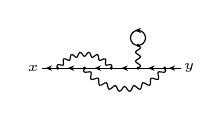
\begin{tikzpicture}[x=0.340cm, y=0.340cm, line width=0.420pt, baseline={([yshift=-0.6ex]0,0)}]
  \draw (-1.000,0.000) -- (-2.000,0.000);
  \fill (-1.619,0.000) -- (-1.381,-0.102) -- (-1.458,0.000) -- (-1.381,0.102) -- cycle;
  \draw (2.000,0.000) -- (1.000,0.000);
  \fill (1.381,0.000) -- (1.619,-0.102) -- (1.542,0.000) -- (1.619,0.102) -- cycle;
  \draw (0.000,0.000) -- (-1.000,0.000);
  \fill (-0.619,0.000) -- (-0.381,-0.102) -- (-0.458,0.000) -- (-0.381,0.102) -- cycle;
  \draw (1.000,0.000) -- (0.000,0.000);
  \fill (0.381,0.000) -- (0.619,-0.102) -- (0.542,0.000) -- (0.619,0.102) -- cycle;
  \draw plot[smooth, tension=0.7] coordinates {(-2.000,0.000) (-2.023,0.066) (-2.017,0.113) (-1.972,0.130) (-1.902,0.122) (-1.834,0.110) (-1.792,0.119) (-1.781,0.162) (-1.790,0.230) (-1.796,0.300) (-1.777,0.344) (-1.730,0.349) (-1.665,0.323) (-1.602,0.295) (-1.558,0.293) (-1.537,0.331) (-1.529,0.400) (-1.516,0.469) (-1.488,0.507) (-1.441,0.499) (-1.384,0.458) (-1.330,0.415) (-1.288,0.402) (-1.258,0.434) (-1.233,0.498) (-1.204,0.561) (-1.166,0.591) (-1.122,0.572) (-1.078,0.518) (-1.037,0.462) (-1.000,0.439) (-0.963,0.462) (-0.922,0.518) (-0.878,0.572) (-0.834,0.591) (-0.796,0.561) (-0.767,0.498) (-0.742,0.434) (-0.712,0.402) (-0.670,0.415) (-0.616,0.458) (-0.559,0.499) (-0.512,0.507) (-0.484,0.469) (-0.471,0.400) (-0.463,0.331) (-0.442,0.293) (-0.398,0.295) (-0.335,0.323) (-0.270,0.349) (-0.223,0.344) (-0.204,0.300) (-0.210,0.230) (-0.219,0.162) (-0.208,0.119) (-0.166,0.110) (-0.098,0.122) (-0.028,0.130) (0.017,0.113) (0.023,0.066) (0.000,0.000)};
  \draw plot[smooth, tension=0.7] coordinates {(2.000,0.000) (2.028,-0.078) (2.021,-0.133) (1.969,-0.154) (1.886,-0.146) (1.805,-0.135) (1.755,-0.148) (1.744,-0.199) (1.759,-0.279) (1.770,-0.361) (1.752,-0.414) (1.697,-0.424) (1.618,-0.399) (1.541,-0.372) (1.488,-0.375) (1.468,-0.423) (1.466,-0.505) (1.461,-0.587) (1.433,-0.636) (1.377,-0.634) (1.304,-0.594) (1.234,-0.552) (1.182,-0.544) (1.152,-0.587) (1.134,-0.667) (1.112,-0.747) (1.075,-0.788) (1.021,-0.775) (0.958,-0.722) (0.897,-0.667) (0.848,-0.649) (0.810,-0.685) (0.776,-0.759) (0.739,-0.833) (0.694,-0.866) (0.644,-0.843) (0.592,-0.778) (0.545,-0.711) (0.500,-0.684) (0.455,-0.711) (0.408,-0.778) (0.356,-0.843) (0.306,-0.866) (0.261,-0.833) (0.224,-0.759) (0.190,-0.685) (0.152,-0.649) (0.103,-0.667) (0.042,-0.722) (-0.021,-0.775) (-0.075,-0.788) (-0.112,-0.747) (-0.134,-0.667) (-0.152,-0.587) (-0.182,-0.544) (-0.234,-0.552) (-0.304,-0.594) (-0.377,-0.634) (-0.433,-0.636) (-0.461,-0.587) (-0.466,-0.505) (-0.468,-0.423) (-0.488,-0.375) (-0.541,-0.372) (-0.618,-0.399) (-0.697,-0.424) (-0.752,-0.414) (-0.770,-0.361) (-0.759,-0.279) (-0.744,-0.199) (-0.755,-0.148) (-0.805,-0.135) (-0.886,-0.146) (-0.969,-0.154) (-1.021,-0.133) (-1.028,-0.078) (-1.000,0.000)};
  \draw plot[smooth, tension=0.7] coordinates {(1.000,0.850) (1.065,0.808) (1.092,0.765) (1.065,0.722) (1.000,0.680) (0.935,0.638) (0.908,0.595) (0.935,0.552) (1.000,0.510) (1.065,0.467) (1.092,0.425) (1.065,0.382) (1.000,0.340) (0.935,0.298) (0.908,0.255) (0.935,0.213) (1.000,0.170) (1.065,0.127) (1.092,0.085) (1.065,0.042) (1.000,0.000)};
  \draw (1.000,0.850) arc[start angle=270.000, end angle=630.000, radius=0.280];
  \fill (0.881,1.410) -- (1.119,1.308) -- (1.042,1.410) -- (1.119,1.512) -- cycle;
  \draw (-2.000,0.000) -- (-2.600,0.000);
  \fill (-2.449,0.000) -- (-2.211,-0.102) -- (-2.288,0.000) -- (-2.211,0.102) -- cycle;
  \draw (2.000,0.000) -- (2.600,0.000);
  \fill (2.151,0.000) -- (2.389,-0.102) -- (2.312,0.000) -- (2.389,0.102) -- cycle;
  \fill (-2.000,0.000) circle (0.064);
  \fill (2.000,0.000) circle (0.064);
  \fill (1.000,0.850) circle (0.064);
  \fill (1.000,0.000) circle (0.064);
  \fill (-1.000,0.000) circle (0.064);
  \fill (0.000,0.000) circle (0.064);
  \node[font=\tiny, inner sep=0pt, anchor=0] at (-2.690,0.000) {$x$};
  \node[font=\tiny, inner sep=0pt, anchor=180] at (2.690,0.000) {$y$};
\end{tikzpicture}}
\diagramgap
\mbox{$\displaystyle +\,$\,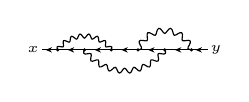
\begin{tikzpicture}[x=0.340cm, y=0.340cm, line width=0.420pt, baseline={([yshift=-0.6ex]0,0)}]
  \draw (-1.500,0.000) -- (-2.500,0.000);
  \fill (-2.119,0.000) -- (-1.881,-0.102) -- (-1.958,0.000) -- (-1.881,0.102) -- cycle;
  \draw (2.500,0.000) -- (1.500,0.000);
  \fill (1.881,0.000) -- (2.119,-0.102) -- (2.042,0.000) -- (2.119,0.102) -- cycle;
  \draw (-0.500,0.000) -- (-1.500,0.000);
  \fill (-1.119,0.000) -- (-0.881,-0.102) -- (-0.958,0.000) -- (-0.881,0.102) -- cycle;
  \draw (0.500,0.000) -- (-0.500,0.000);
  \fill (-0.119,0.000) -- (0.119,-0.102) -- (0.042,0.000) -- (0.119,0.102) -- cycle;
  \draw (1.500,0.000) -- (0.500,0.000);
  \fill (0.881,0.000) -- (1.119,-0.102) -- (1.042,0.000) -- (1.119,0.102) -- cycle;
  \draw plot[smooth, tension=0.7] coordinates {(-2.500,0.000) (-2.523,0.066) (-2.517,0.113) (-2.472,0.130) (-2.402,0.122) (-2.334,0.110) (-2.292,0.119) (-2.281,0.162) (-2.290,0.230) (-2.296,0.300) (-2.277,0.344) (-2.230,0.349) (-2.165,0.323) (-2.102,0.295) (-2.058,0.293) (-2.037,0.331) (-2.029,0.400) (-2.016,0.469) (-1.988,0.507) (-1.941,0.499) (-1.884,0.458) (-1.830,0.415) (-1.788,0.402) (-1.758,0.434) (-1.733,0.498) (-1.704,0.561) (-1.666,0.591) (-1.622,0.572) (-1.578,0.518) (-1.537,0.462) (-1.500,0.439) (-1.463,0.462) (-1.422,0.518) (-1.378,0.572) (-1.334,0.591) (-1.296,0.561) (-1.267,0.498) (-1.242,0.434) (-1.212,0.402) (-1.170,0.415) (-1.116,0.458) (-1.059,0.499) (-1.012,0.507) (-0.984,0.469) (-0.971,0.400) (-0.963,0.331) (-0.942,0.293) (-0.898,0.295) (-0.835,0.323) (-0.770,0.349) (-0.723,0.344) (-0.704,0.300) (-0.710,0.230) (-0.719,0.162) (-0.708,0.119) (-0.666,0.110) (-0.598,0.122) (-0.528,0.130) (-0.483,0.113) (-0.477,0.066) (-0.500,0.000)};
  \draw plot[smooth, tension=0.7] coordinates {(2.500,0.000) (2.413,0.021) (2.367,0.052) (2.375,0.107) (2.418,0.185) (2.455,0.268) (2.450,0.331) (2.393,0.357) (2.302,0.350) (2.214,0.337) (2.159,0.348) (2.146,0.402) (2.156,0.491) (2.160,0.582) (2.132,0.638) (2.069,0.641) (1.987,0.601) (1.910,0.556) (1.856,0.546) (1.823,0.591) (1.800,0.677) (1.768,0.762) (1.721,0.804) (1.662,0.783) (1.601,0.715) (1.547,0.644) (1.500,0.615) (1.453,0.644) (1.399,0.715) (1.338,0.783) (1.279,0.804) (1.232,0.762) (1.200,0.677) (1.177,0.591) (1.144,0.546) (1.090,0.556) (1.013,0.601) (0.931,0.641) (0.868,0.638) (0.840,0.582) (0.844,0.491) (0.854,0.402) (0.841,0.348) (0.786,0.337) (0.698,0.350) (0.607,0.357) (0.550,0.331) (0.545,0.268) (0.582,0.185) (0.625,0.107) (0.633,0.052) (0.587,0.021) (0.500,0.000)};
  \draw plot[smooth, tension=0.7] coordinates {(1.500,0.000) (1.528,-0.078) (1.521,-0.133) (1.469,-0.154) (1.386,-0.146) (1.305,-0.135) (1.255,-0.148) (1.244,-0.199) (1.259,-0.279) (1.270,-0.361) (1.252,-0.414) (1.197,-0.424) (1.118,-0.399) (1.041,-0.372) (0.988,-0.375) (0.968,-0.423) (0.966,-0.505) (0.961,-0.587) (0.933,-0.636) (0.877,-0.634) (0.804,-0.594) (0.734,-0.552) (0.682,-0.544) (0.652,-0.587) (0.634,-0.667) (0.612,-0.747) (0.575,-0.788) (0.521,-0.775) (0.458,-0.722) (0.397,-0.667) (0.348,-0.649) (0.310,-0.685) (0.276,-0.759) (0.239,-0.833) (0.194,-0.866) (0.144,-0.843) (0.092,-0.778) (0.045,-0.711) (0.000,-0.684) (-0.045,-0.711) (-0.092,-0.778) (-0.144,-0.843) (-0.194,-0.866) (-0.239,-0.833) (-0.276,-0.759) (-0.310,-0.685) (-0.348,-0.649) (-0.397,-0.667) (-0.458,-0.722) (-0.521,-0.775) (-0.575,-0.788) (-0.612,-0.747) (-0.634,-0.667) (-0.652,-0.587) (-0.682,-0.544) (-0.734,-0.552) (-0.804,-0.594) (-0.877,-0.634) (-0.933,-0.636) (-0.961,-0.587) (-0.966,-0.505) (-0.968,-0.423) (-0.988,-0.375) (-1.041,-0.372) (-1.118,-0.399) (-1.197,-0.424) (-1.252,-0.414) (-1.270,-0.361) (-1.259,-0.279) (-1.244,-0.199) (-1.255,-0.148) (-1.305,-0.135) (-1.386,-0.146) (-1.469,-0.154) (-1.521,-0.133) (-1.528,-0.078) (-1.500,0.000)};
  \draw (-2.500,0.000) -- (-3.100,0.000);
  \fill (-2.949,0.000) -- (-2.711,-0.102) -- (-2.788,0.000) -- (-2.711,0.102) -- cycle;
  \draw (2.500,0.000) -- (3.100,0.000);
  \fill (2.651,0.000) -- (2.889,-0.102) -- (2.812,0.000) -- (2.889,0.102) -- cycle;
  \fill (-2.500,0.000) circle (0.064);
  \fill (2.500,0.000) circle (0.064);
  \fill (1.500,0.000) circle (0.064);
  \fill (-1.500,0.000) circle (0.064);
  \fill (-0.500,0.000) circle (0.064);
  \fill (0.500,0.000) circle (0.064);
  \node[font=\tiny, inner sep=0pt, anchor=0] at (-3.190,0.000) {$x$};
  \node[font=\tiny, inner sep=0pt, anchor=180] at (3.190,0.000) {$y$};
\end{tikzpicture}}
\diagramgap
\mbox{$\displaystyle +\,$\,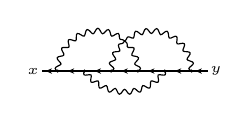
\begin{tikzpicture}[x=0.340cm, y=0.340cm, line width=0.420pt, baseline={([yshift=-0.6ex]0,0)}]
  \draw (-1.500,0.000) -- (-2.500,0.000);
  \fill (-2.119,0.000) -- (-1.881,-0.102) -- (-1.958,0.000) -- (-1.881,0.102) -- cycle;
  \draw (2.500,0.000) -- (1.500,0.000);
  \fill (1.881,0.000) -- (2.119,-0.102) -- (2.042,0.000) -- (2.119,0.102) -- cycle;
  \draw (-0.500,0.000) -- (-1.500,0.000);
  \fill (-1.119,0.000) -- (-0.881,-0.102) -- (-0.958,0.000) -- (-0.881,0.102) -- cycle;
  \draw (1.500,0.000) -- (0.500,0.000);
  \fill (0.881,0.000) -- (1.119,-0.102) -- (1.042,0.000) -- (1.119,0.102) -- cycle;
  \draw (0.500,0.000) -- (-0.500,0.000);
  \fill (-0.119,0.000) -- (0.119,-0.102) -- (0.042,0.000) -- (0.119,0.102) -- cycle;
  \draw plot[smooth, tension=0.7] coordinates {(-2.500,0.000) (-2.569,0.049) (-2.595,0.100) (-2.562,0.148) (-2.488,0.188) (-2.413,0.224) (-2.377,0.263) (-2.396,0.312) (-2.453,0.373) (-2.507,0.438) (-2.520,0.494) (-2.477,0.532) (-2.395,0.552) (-2.313,0.568) (-2.269,0.597) (-2.275,0.650) (-2.314,0.723) (-2.351,0.799) (-2.349,0.856) (-2.298,0.882) (-2.214,0.882) (-2.130,0.877) (-2.080,0.894) (-2.073,0.946) (-2.093,1.027) (-2.110,1.110) (-2.094,1.165) (-2.038,1.177) (-1.956,1.156) (-1.877,1.130) (-1.824,1.134) (-1.804,1.183) (-1.804,1.266) (-1.799,1.351) (-1.770,1.400) (-1.712,1.398) (-1.639,1.357) (-1.568,1.313) (-1.516,1.304) (-1.485,1.346) (-1.464,1.427) (-1.438,1.507) (-1.397,1.548) (-1.342,1.532) (-1.281,1.473) (-1.224,1.413) (-1.176,1.391) (-1.135,1.424) (-1.094,1.497) (-1.049,1.569) (-1.000,1.598) (-0.951,1.569) (-0.906,1.497) (-0.865,1.424) (-0.824,1.391) (-0.776,1.413) (-0.719,1.473) (-0.658,1.532) (-0.603,1.548) (-0.562,1.507) (-0.536,1.427) (-0.515,1.346) (-0.484,1.304) (-0.432,1.313) (-0.361,1.357) (-0.288,1.398) (-0.230,1.400) (-0.203,1.348) (-0.196,1.266) (-0.182,1.204) (-0.143,1.179) (-0.091,1.172) (-0.044,1.156) (-0.008,1.125) (0.029,1.096) (0.068,1.068) (0.093,1.027) (0.098,0.968) (0.101,0.911) (0.136,0.881) (0.214,0.882) (0.298,0.882) (0.349,0.856) (0.351,0.799) (0.314,0.723) (0.275,0.650) (0.269,0.597) (0.313,0.568) (0.395,0.552) (0.477,0.532) (0.520,0.494) (0.507,0.438) (0.453,0.373) (0.396,0.312) (0.377,0.263) (0.413,0.224) (0.488,0.188) (0.562,0.148) (0.595,0.100) (0.569,0.049) (0.500,0.000)};
  \draw plot[smooth, tension=0.7] coordinates {(2.500,0.000) (2.430,0.045) (2.399,0.088) (2.424,0.135) (2.488,0.188) (2.550,0.245) (2.570,0.299) (2.532,0.342) (2.453,0.373) (2.374,0.399) (2.333,0.433) (2.346,0.485) (2.395,0.552) (2.440,0.623) (2.446,0.680) (2.398,0.712) (2.314,0.723) (2.231,0.728) (2.184,0.751) (2.183,0.804) (2.214,0.882) (2.240,0.962) (2.231,1.019) (2.177,1.038) (2.093,1.027) (2.012,1.012) (1.960,1.022) (1.946,1.073) (1.956,1.156) (1.962,1.240) (1.939,1.293) (1.882,1.298) (1.804,1.266) (1.728,1.231) (1.675,1.229) (1.650,1.275) (1.639,1.357) (1.623,1.440) (1.588,1.486) (1.532,1.477) (1.464,1.427) (1.399,1.374) (1.349,1.358) (1.312,1.396) (1.281,1.473) (1.245,1.550) (1.200,1.585) (1.148,1.562) (1.094,1.497) (1.045,1.430) (1.000,1.402) (0.955,1.430) (0.906,1.497) (0.852,1.562) (0.800,1.585) (0.755,1.550) (0.719,1.473) (0.688,1.396) (0.651,1.358) (0.601,1.374) (0.536,1.427) (0.468,1.477) (0.412,1.486) (0.377,1.440) (0.361,1.357) (0.350,1.275) (0.325,1.229) (0.270,1.234) (0.196,1.266) (0.132,1.277) (0.094,1.248) (0.071,1.198) (0.044,1.156) (0.008,1.125) (-0.025,1.091) (-0.053,1.053) (-0.093,1.027) (-0.153,1.016) (-0.211,1.002) (-0.234,0.957) (-0.214,0.882) (-0.183,0.804) (-0.184,0.751) (-0.231,0.728) (-0.314,0.723) (-0.398,0.712) (-0.446,0.680) (-0.440,0.623) (-0.395,0.552) (-0.346,0.485) (-0.333,0.433) (-0.374,0.399) (-0.453,0.373) (-0.532,0.342) (-0.570,0.299) (-0.550,0.245) (-0.488,0.188) (-0.424,0.135) (-0.399,0.088) (-0.430,0.045) (-0.500,0.000)};
  \draw plot[smooth, tension=0.7] coordinates {(1.500,0.000) (1.528,-0.078) (1.521,-0.133) (1.469,-0.154) (1.386,-0.146) (1.305,-0.135) (1.255,-0.148) (1.244,-0.199) (1.259,-0.279) (1.270,-0.361) (1.252,-0.414) (1.197,-0.424) (1.118,-0.399) (1.041,-0.372) (0.988,-0.375) (0.968,-0.423) (0.966,-0.505) (0.961,-0.587) (0.933,-0.636) (0.877,-0.634) (0.804,-0.594) (0.734,-0.552) (0.682,-0.544) (0.652,-0.587) (0.634,-0.667) (0.612,-0.747) (0.575,-0.788) (0.521,-0.775) (0.458,-0.722) (0.397,-0.667) (0.348,-0.649) (0.310,-0.685) (0.276,-0.759) (0.239,-0.833) (0.194,-0.866) (0.144,-0.843) (0.092,-0.778) (0.045,-0.711) (0.000,-0.684) (-0.045,-0.711) (-0.092,-0.778) (-0.144,-0.843) (-0.194,-0.866) (-0.239,-0.833) (-0.276,-0.759) (-0.310,-0.685) (-0.348,-0.649) (-0.397,-0.667) (-0.458,-0.722) (-0.521,-0.775) (-0.575,-0.788) (-0.612,-0.747) (-0.634,-0.667) (-0.652,-0.587) (-0.682,-0.544) (-0.734,-0.552) (-0.804,-0.594) (-0.877,-0.634) (-0.933,-0.636) (-0.961,-0.587) (-0.966,-0.505) (-0.968,-0.423) (-0.988,-0.375) (-1.041,-0.372) (-1.118,-0.399) (-1.197,-0.424) (-1.252,-0.414) (-1.270,-0.361) (-1.259,-0.279) (-1.244,-0.199) (-1.255,-0.148) (-1.305,-0.135) (-1.386,-0.146) (-1.469,-0.154) (-1.521,-0.133) (-1.528,-0.078) (-1.500,0.000)};
  \draw (-2.500,0.000) -- (-3.100,0.000);
  \fill (-2.949,0.000) -- (-2.711,-0.102) -- (-2.788,0.000) -- (-2.711,0.102) -- cycle;
  \draw (2.500,0.000) -- (3.100,0.000);
  \fill (2.651,0.000) -- (2.889,-0.102) -- (2.812,0.000) -- (2.889,0.102) -- cycle;
  \fill (-2.500,0.000) circle (0.064);
  \fill (2.500,0.000) circle (0.064);
  \fill (1.500,0.000) circle (0.064);
  \fill (-1.500,0.000) circle (0.064);
  \fill (0.500,0.000) circle (0.064);
  \fill (-0.500,0.000) circle (0.064);
  \node[font=\tiny, inner sep=0pt, anchor=0] at (-3.190,0.000) {$x$};
  \node[font=\tiny, inner sep=0pt, anchor=180] at (3.190,0.000) {$y$};
\end{tikzpicture}}
\diagramgap
\mbox{$\displaystyle +\,$\,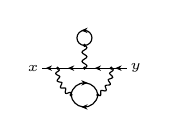
\begin{tikzpicture}[x=0.340cm, y=0.340cm, line width=0.420pt, baseline={([yshift=-0.6ex]0,0)}]
  \draw (0.000,0.000) -- (-1.000,0.000);
  \fill (-0.619,0.000) -- (-0.381,-0.102) -- (-0.458,0.000) -- (-0.381,0.102) -- cycle;
  \draw (1.000,0.000) -- (0.000,0.000);
  \fill (0.381,0.000) -- (0.619,-0.102) -- (0.542,0.000) -- (0.619,0.102) -- cycle;
  \draw (0.500,-1.000) arc[start angle=353.974, end angle=186.026, radius=0.503];
  \fill (-0.119,-1.450) -- (0.119,-1.552) -- (0.042,-1.450) -- (0.119,-1.348) -- cycle;
  \draw (-0.500,-1.000) arc[start angle=173.974, end angle=6.026, radius=0.503];
  \fill (0.119,-0.550) -- (-0.119,-0.448) -- (-0.042,-0.550) -- (-0.119,-0.652) -- cycle;
  \draw plot[smooth, tension=0.7] coordinates {(-1.000,0.000) (-0.955,-0.037) (-0.938,-0.070) (-0.959,-0.100) (-1.008,-0.131) (-1.056,-0.166) (-1.074,-0.202) (-1.051,-0.235) (-0.999,-0.263) (-0.947,-0.287) (-0.921,-0.314) (-0.934,-0.349) (-0.973,-0.392) (-1.010,-0.438) (-1.019,-0.477) (-0.988,-0.503) (-0.930,-0.517) (-0.873,-0.526) (-0.841,-0.546) (-0.845,-0.583) (-0.871,-0.634) (-0.895,-0.688) (-0.893,-0.729) (-0.857,-0.746) (-0.798,-0.743) (-0.740,-0.738) (-0.704,-0.748) (-0.698,-0.785) (-0.710,-0.842) (-0.719,-0.900) (-0.706,-0.938) (-0.667,-0.945) (-0.610,-0.928) (-0.556,-0.908) (-0.519,-0.908) (-0.503,-0.942) (-0.500,-1.000)};
  \draw plot[smooth, tension=0.7] coordinates {(1.000,0.000) (1.052,-0.028) (1.075,-0.061) (1.056,-0.097) (1.008,-0.131) (0.959,-0.163) (0.938,-0.193) (0.955,-0.225) (0.999,-0.263) (1.042,-0.304) (1.056,-0.341) (1.029,-0.371) (0.973,-0.392) (0.918,-0.409) (0.889,-0.433) (0.897,-0.469) (0.930,-0.517) (0.961,-0.567) (0.964,-0.607) (0.930,-0.629) (0.871,-0.634) (0.813,-0.637) (0.780,-0.652) (0.778,-0.689) (0.798,-0.743) (0.814,-0.800) (0.807,-0.840) (0.768,-0.852) (0.710,-0.842) (0.653,-0.829) (0.617,-0.835) (0.606,-0.870) (0.610,-0.928) (0.611,-0.987) (0.594,-1.023) (0.554,-1.025) (0.500,-1.000)};
  \draw plot[smooth, tension=0.7] coordinates {(0.000,0.850) (0.065,0.808) (0.092,0.765) (0.065,0.722) (0.000,0.680) (-0.065,0.638) (-0.092,0.595) (-0.065,0.552) (0.000,0.510) (0.065,0.467) (0.092,0.425) (0.065,0.382) (0.000,0.340) (-0.065,0.298) (-0.092,0.255) (-0.065,0.213) (0.000,0.170) (0.065,0.127) (0.092,0.085) (0.065,0.042) (0.000,0.000)};
  \draw (0.000,0.850) arc[start angle=270.000, end angle=630.000, radius=0.280];
  \fill (-0.119,1.410) -- (0.119,1.308) -- (0.042,1.410) -- (0.119,1.512) -- cycle;
  \draw (-1.000,0.000) -- (-1.600,0.000);
  \fill (-1.449,0.000) -- (-1.211,-0.102) -- (-1.288,0.000) -- (-1.211,0.102) -- cycle;
  \draw (1.000,0.000) -- (1.600,0.000);
  \fill (1.151,0.000) -- (1.389,-0.102) -- (1.312,0.000) -- (1.389,0.102) -- cycle;
  \fill (-1.000,0.000) circle (0.064);
  \fill (1.000,0.000) circle (0.064);
  \fill (0.000,0.850) circle (0.064);
  \fill (0.000,0.000) circle (0.064);
  \fill (-0.500,-1.000) circle (0.064);
  \fill (0.500,-1.000) circle (0.064);
  \node[font=\tiny, inner sep=0pt, anchor=0] at (-1.690,0.000) {$x$};
  \node[font=\tiny, inner sep=0pt, anchor=180] at (1.690,0.000) {$y$};
\end{tikzpicture}}
\diagramgap
\mbox{$\displaystyle -\,$\,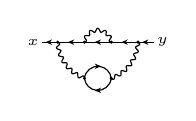
\begin{tikzpicture}[x=0.340cm, y=0.340cm, line width=0.420pt, baseline={([yshift=-0.6ex]0,0)}]
  \draw (-0.500,0.000) -- (-1.500,0.000);
  \fill (-1.119,0.000) -- (-0.881,-0.102) -- (-0.958,0.000) -- (-0.881,0.102) -- cycle;
  \draw (1.500,0.000) -- (0.500,0.000);
  \fill (0.881,0.000) -- (1.119,-0.102) -- (1.042,0.000) -- (1.119,0.102) -- cycle;
  \draw (0.500,0.000) -- (-0.500,0.000);
  \fill (-0.119,0.000) -- (0.119,-0.102) -- (0.042,0.000) -- (0.119,0.102) -- cycle;
  \draw plot[smooth, tension=0.7] coordinates {(0.500,0.000) (0.447,0.025) (0.421,0.050) (0.433,0.083) (0.468,0.130) (0.500,0.181) (0.501,0.224) (0.464,0.246) (0.404,0.247) (0.345,0.241) (0.311,0.249) (0.303,0.284) (0.311,0.342) (0.312,0.403) (0.291,0.440) (0.248,0.440) (0.196,0.410) (0.148,0.376) (0.114,0.365) (0.090,0.392) (0.067,0.446) (0.037,0.498) (0.000,0.520) (-0.037,0.498) (-0.067,0.446) (-0.090,0.392) (-0.114,0.365) (-0.148,0.376) (-0.196,0.410) (-0.248,0.440) (-0.291,0.440) (-0.312,0.403) (-0.311,0.342) (-0.303,0.284) (-0.311,0.249) (-0.345,0.241) (-0.404,0.247) (-0.464,0.246) (-0.501,0.224) (-0.500,0.181) (-0.468,0.130) (-0.433,0.083) (-0.421,0.050) (-0.447,0.025) (-0.500,0.000)};
  \draw (0.500,-1.350) arc[start angle=353.974, end angle=186.026, radius=0.503];
  \fill (-0.119,-1.800) -- (0.119,-1.902) -- (0.042,-1.800) -- (0.119,-1.698) -- cycle;
  \draw (-0.500,-1.350) arc[start angle=173.974, end angle=6.026, radius=0.503];
  \fill (0.119,-0.900) -- (-0.119,-0.798) -- (-0.042,-0.900) -- (-0.119,-1.002) -- cycle;
  \draw plot[smooth, tension=0.7] coordinates {(-1.500,0.000) (-1.448,-0.031) (-1.424,-0.062) (-1.442,-0.097) (-1.487,-0.136) (-1.532,-0.178) (-1.547,-0.217) (-1.519,-0.248) (-1.462,-0.271) (-1.405,-0.292) (-1.377,-0.318) (-1.388,-0.356) (-1.425,-0.403) (-1.462,-0.452) (-1.469,-0.493) (-1.436,-0.519) (-1.376,-0.531) (-1.317,-0.541) (-1.284,-0.562) (-1.287,-0.601) (-1.316,-0.654) (-1.343,-0.709) (-1.343,-0.750) (-1.306,-0.770) (-1.245,-0.771) (-1.184,-0.770) (-1.148,-0.785) (-1.145,-0.824) (-1.163,-0.881) (-1.180,-0.940) (-1.172,-0.981) (-1.133,-0.993) (-1.072,-0.983) (-1.013,-0.972) (-0.974,-0.979) (-0.964,-1.017) (-0.972,-1.077) (-0.977,-1.138) (-0.963,-1.177) (-0.922,-1.182) (-0.864,-1.161) (-0.807,-1.139) (-0.769,-1.139) (-0.752,-1.174) (-0.748,-1.235) (-0.743,-1.296) (-0.721,-1.331) (-0.680,-1.329) (-0.627,-1.298) (-0.575,-1.266) (-0.537,-1.260) (-0.514,-1.291) (-0.500,-1.350)};
  \draw plot[smooth, tension=0.7] coordinates {(1.500,0.000) (1.548,-0.038) (1.566,-0.075) (1.542,-0.108) (1.487,-0.136) (1.433,-0.162) (1.406,-0.191) (1.420,-0.227) (1.462,-0.271) (1.503,-0.317) (1.514,-0.357) (1.484,-0.385) (1.425,-0.403) (1.367,-0.419) (1.336,-0.442) (1.343,-0.480) (1.376,-0.531) (1.408,-0.583) (1.412,-0.625) (1.377,-0.647) (1.316,-0.654) (1.256,-0.659) (1.221,-0.676) (1.221,-0.715) (1.245,-0.771) (1.267,-0.828) (1.263,-0.870) (1.224,-0.885) (1.163,-0.881) (1.103,-0.875) (1.066,-0.886) (1.059,-0.924) (1.072,-0.983) (1.083,-1.044) (1.072,-1.083) (1.031,-1.092) (0.972,-1.077) (0.914,-1.060) (0.875,-1.064) (0.862,-1.101) (0.864,-1.161) (0.864,-1.222) (0.845,-1.259) (0.804,-1.261) (0.748,-1.235) (0.694,-1.208) (0.656,-1.205) (0.636,-1.238) (0.627,-1.298) (0.616,-1.358) (0.591,-1.391) (0.550,-1.385) (0.500,-1.350)};
  \draw (-1.500,0.000) -- (-2.100,0.000);
  \fill (-1.949,0.000) -- (-1.711,-0.102) -- (-1.788,0.000) -- (-1.711,0.102) -- cycle;
  \draw (1.500,0.000) -- (2.100,0.000);
  \fill (1.651,0.000) -- (1.889,-0.102) -- (1.812,0.000) -- (1.889,0.102) -- cycle;
  \fill (-1.500,0.000) circle (0.064);
  \fill (1.500,0.000) circle (0.064);
  \fill (0.500,0.000) circle (0.064);
  \fill (-0.500,0.000) circle (0.064);
  \fill (-0.500,-1.350) circle (0.064);
  \fill (0.500,-1.350) circle (0.064);
  \node[font=\tiny, inner sep=0pt, anchor=0] at (-2.190,0.000) {$x$};
  \node[font=\tiny, inner sep=0pt, anchor=180] at (2.190,0.000) {$y$};
\end{tikzpicture}}
\diagramgap
\mbox{$\displaystyle -\,$\,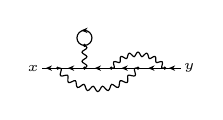
\begin{tikzpicture}[x=0.340cm, y=0.340cm, line width=0.420pt, baseline={([yshift=-0.6ex]0,0)}]
  \draw (-1.000,0.000) -- (-2.000,0.000);
  \fill (-1.619,0.000) -- (-1.381,-0.102) -- (-1.458,0.000) -- (-1.381,0.102) -- cycle;
  \draw (2.000,0.000) -- (1.000,0.000);
  \fill (1.381,0.000) -- (1.619,-0.102) -- (1.542,0.000) -- (1.619,0.102) -- cycle;
  \draw (0.000,0.000) -- (-1.000,0.000);
  \fill (-0.619,0.000) -- (-0.381,-0.102) -- (-0.458,0.000) -- (-0.381,0.102) -- cycle;
  \draw (1.000,0.000) -- (0.000,0.000);
  \fill (0.381,0.000) -- (0.619,-0.102) -- (0.542,0.000) -- (0.619,0.102) -- cycle;
  \draw plot[smooth, tension=0.7] coordinates {(-2.000,0.000) (-1.918,0.003) (-1.869,-0.015) (-1.864,-0.067) (-1.886,-0.146) (-1.906,-0.226) (-1.894,-0.281) (-1.840,-0.295) (-1.759,-0.279) (-1.679,-0.260) (-1.627,-0.268) (-1.611,-0.318) (-1.618,-0.399) (-1.621,-0.482) (-1.598,-0.533) (-1.542,-0.537) (-1.466,-0.505) (-1.392,-0.470) (-1.340,-0.467) (-1.314,-0.513) (-1.304,-0.594) (-1.291,-0.676) (-1.258,-0.721) (-1.202,-0.713) (-1.134,-0.667) (-1.069,-0.618) (-1.018,-0.605) (-0.984,-0.644) (-0.958,-0.722) (-0.928,-0.799) (-0.887,-0.837) (-0.834,-0.818) (-0.776,-0.759) (-0.722,-0.698) (-0.675,-0.675) (-0.633,-0.707) (-0.592,-0.778) (-0.548,-0.847) (-0.500,-0.876) (-0.452,-0.847) (-0.408,-0.778) (-0.367,-0.707) (-0.325,-0.675) (-0.278,-0.698) (-0.224,-0.759) (-0.166,-0.818) (-0.113,-0.837) (-0.072,-0.799) (-0.042,-0.722) (-0.016,-0.644) (0.018,-0.605) (0.069,-0.618) (0.134,-0.667) (0.202,-0.713) (0.258,-0.721) (0.291,-0.676) (0.304,-0.594) (0.314,-0.513) (0.340,-0.467) (0.392,-0.470) (0.466,-0.505) (0.542,-0.537) (0.598,-0.533) (0.621,-0.482) (0.618,-0.399) (0.611,-0.318) (0.627,-0.268) (0.679,-0.260) (0.759,-0.279) (0.840,-0.295) (0.894,-0.281) (0.906,-0.226) (0.886,-0.146) (0.864,-0.067) (0.869,-0.015) (0.918,0.003) (1.000,0.000)};
  \draw plot[smooth, tension=0.7] coordinates {(2.000,0.000) (1.931,-0.003) (1.890,0.012) (1.885,0.055) (1.902,0.122) (1.917,0.190) (1.904,0.236) (1.858,0.247) (1.790,0.230) (1.724,0.210) (1.680,0.214) (1.664,0.254) (1.665,0.323) (1.661,0.393) (1.638,0.434) (1.590,0.433) (1.529,0.400) (1.470,0.363) (1.427,0.356) (1.401,0.391) (1.384,0.458) (1.363,0.525) (1.330,0.559) (1.284,0.546) (1.233,0.498) (1.185,0.448) (1.145,0.429) (1.111,0.457) (1.078,0.518) (1.041,0.577) (1.000,0.601) (0.959,0.577) (0.922,0.518) (0.889,0.457) (0.855,0.429) (0.815,0.448) (0.767,0.498) (0.716,0.546) (0.670,0.559) (0.637,0.525) (0.616,0.458) (0.599,0.391) (0.573,0.356) (0.530,0.363) (0.471,0.400) (0.410,0.433) (0.362,0.434) (0.339,0.393) (0.335,0.323) (0.336,0.254) (0.320,0.214) (0.276,0.210) (0.210,0.230) (0.142,0.247) (0.096,0.236) (0.083,0.190) (0.098,0.122) (0.115,0.055) (0.110,0.012) (0.069,-0.003) (0.000,0.000)};
  \draw plot[smooth, tension=0.7] coordinates {(-1.000,0.850) (-0.935,0.808) (-0.908,0.765) (-0.935,0.722) (-1.000,0.680) (-1.065,0.638) (-1.092,0.595) (-1.065,0.552) (-1.000,0.510) (-0.935,0.467) (-0.908,0.425) (-0.935,0.382) (-1.000,0.340) (-1.065,0.298) (-1.092,0.255) (-1.065,0.213) (-1.000,0.170) (-0.935,0.127) (-0.908,0.085) (-0.935,0.042) (-1.000,0.000)};
  \draw (-1.000,0.850) arc[start angle=270.000, end angle=630.000, radius=0.280];
  \fill (-1.119,1.410) -- (-0.881,1.308) -- (-0.958,1.410) -- (-0.881,1.512) -- cycle;
  \draw (-2.000,0.000) -- (-2.600,0.000);
  \fill (-2.449,0.000) -- (-2.211,-0.102) -- (-2.288,0.000) -- (-2.211,0.102) -- cycle;
  \draw (2.000,0.000) -- (2.600,0.000);
  \fill (2.151,0.000) -- (2.389,-0.102) -- (2.312,0.000) -- (2.389,0.102) -- cycle;
  \fill (-2.000,0.000) circle (0.064);
  \fill (2.000,0.000) circle (0.064);
  \fill (-1.000,0.850) circle (0.064);
  \fill (1.000,0.000) circle (0.064);
  \fill (-1.000,0.000) circle (0.064);
  \fill (0.000,0.000) circle (0.064);
  \node[font=\tiny, inner sep=0pt, anchor=0] at (-2.690,0.000) {$x$};
  \node[font=\tiny, inner sep=0pt, anchor=180] at (2.690,0.000) {$y$};
\end{tikzpicture}}
\diagramgap
\mbox{$\displaystyle +\,$\,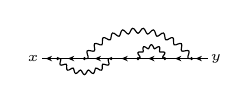
\begin{tikzpicture}[x=0.340cm, y=0.340cm, line width=0.420pt, baseline={([yshift=-0.6ex]0,0)}]
  \draw (-1.500,0.000) -- (-2.500,0.000);
  \fill (-2.119,0.000) -- (-1.881,-0.102) -- (-1.958,0.000) -- (-1.881,0.102) -- cycle;
  \draw (2.500,0.000) -- (1.500,0.000);
  \fill (1.881,0.000) -- (2.119,-0.102) -- (2.042,0.000) -- (2.119,0.102) -- cycle;
  \draw (-0.500,0.000) -- (-1.500,0.000);
  \fill (-1.119,0.000) -- (-0.881,-0.102) -- (-0.958,0.000) -- (-0.881,0.102) -- cycle;
  \draw (0.500,0.000) -- (-0.500,0.000);
  \fill (-0.119,0.000) -- (0.119,-0.102) -- (0.042,0.000) -- (0.119,0.102) -- cycle;
  \draw (1.500,0.000) -- (0.500,0.000);
  \fill (0.881,0.000) -- (1.119,-0.102) -- (1.042,0.000) -- (1.119,0.102) -- cycle;
  \draw plot[smooth, tension=0.7] coordinates {(1.500,0.000) (1.447,0.025) (1.421,0.050) (1.433,0.083) (1.468,0.130) (1.500,0.181) (1.501,0.224) (1.464,0.246) (1.404,0.247) (1.345,0.241) (1.311,0.249) (1.303,0.284) (1.311,0.342) (1.312,0.403) (1.291,0.440) (1.248,0.440) (1.196,0.410) (1.148,0.376) (1.114,0.365) (1.090,0.392) (1.067,0.446) (1.037,0.498) (1.000,0.520) (0.963,0.498) (0.933,0.446) (0.910,0.392) (0.886,0.365) (0.852,0.376) (0.804,0.410) (0.752,0.440) (0.709,0.440) (0.688,0.403) (0.689,0.342) (0.697,0.284) (0.689,0.249) (0.655,0.241) (0.596,0.247) (0.536,0.246) (0.499,0.224) (0.500,0.181) (0.532,0.130) (0.567,0.083) (0.579,0.050) (0.553,0.025) (0.500,0.000)};
  \draw plot[smooth, tension=0.7] coordinates {(-2.500,0.000) (-2.431,0.003) (-2.390,-0.012) (-2.385,-0.055) (-2.402,-0.122) (-2.417,-0.190) (-2.404,-0.236) (-2.358,-0.247) (-2.290,-0.230) (-2.224,-0.210) (-2.180,-0.214) (-2.164,-0.254) (-2.165,-0.323) (-2.161,-0.393) (-2.138,-0.434) (-2.090,-0.433) (-2.029,-0.400) (-1.970,-0.363) (-1.927,-0.356) (-1.901,-0.391) (-1.884,-0.458) (-1.863,-0.525) (-1.830,-0.559) (-1.784,-0.546) (-1.733,-0.498) (-1.685,-0.448) (-1.645,-0.429) (-1.611,-0.457) (-1.578,-0.518) (-1.541,-0.577) (-1.500,-0.601) (-1.459,-0.577) (-1.422,-0.518) (-1.389,-0.457) (-1.355,-0.429) (-1.315,-0.448) (-1.267,-0.498) (-1.216,-0.546) (-1.170,-0.559) (-1.137,-0.525) (-1.116,-0.458) (-1.099,-0.391) (-1.073,-0.356) (-1.030,-0.363) (-0.971,-0.400) (-0.910,-0.433) (-0.862,-0.434) (-0.839,-0.393) (-0.835,-0.323) (-0.836,-0.254) (-0.820,-0.214) (-0.776,-0.210) (-0.710,-0.230) (-0.642,-0.247) (-0.596,-0.236) (-0.583,-0.190) (-0.598,-0.122) (-0.615,-0.055) (-0.610,-0.012) (-0.569,0.003) (-0.500,0.000)};
  \draw plot[smooth, tension=0.7] coordinates {(2.500,0.000) (2.417,-0.003) (2.367,0.017) (2.362,0.070) (2.387,0.149) (2.409,0.230) (2.398,0.285) (2.345,0.302) (2.262,0.289) (2.180,0.274) (2.128,0.285) (2.115,0.337) (2.127,0.419) (2.137,0.502) (2.118,0.555) (2.063,0.564) (1.983,0.539) (1.904,0.511) (1.851,0.514) (1.830,0.564) (1.829,0.647) (1.826,0.730) (1.800,0.780) (1.744,0.780) (1.668,0.742) (1.595,0.703) (1.542,0.698) (1.514,0.744) (1.501,0.826) (1.485,0.908) (1.451,0.953) (1.395,0.944) (1.327,0.896) (1.261,0.846) (1.209,0.833) (1.174,0.873) (1.148,0.952) (1.120,1.031) (1.080,1.070) (1.026,1.053) (0.966,0.995) (0.908,0.936) (0.859,0.915) (0.818,0.950) (0.781,1.024) (0.741,1.097) (0.695,1.130) (0.644,1.105) (0.594,1.038) (0.546,0.971) (0.500,0.943) (0.454,0.971) (0.406,1.038) (0.356,1.105) (0.305,1.130) (0.259,1.097) (0.219,1.024) (0.182,0.950) (0.141,0.915) (0.092,0.936) (0.034,0.995) (-0.026,1.053) (-0.080,1.070) (-0.120,1.031) (-0.148,0.952) (-0.174,0.873) (-0.209,0.833) (-0.261,0.846) (-0.327,0.896) (-0.395,0.944) (-0.451,0.953) (-0.485,0.908) (-0.501,0.826) (-0.514,0.744) (-0.542,0.698) (-0.595,0.703) (-0.668,0.742) (-0.744,0.780) (-0.800,0.780) (-0.826,0.730) (-0.829,0.647) (-0.830,0.564) (-0.851,0.514) (-0.904,0.511) (-0.983,0.539) (-1.063,0.564) (-1.118,0.555) (-1.137,0.502) (-1.127,0.419) (-1.115,0.337) (-1.128,0.285) (-1.180,0.274) (-1.262,0.289) (-1.345,0.302) (-1.398,0.285) (-1.409,0.230) (-1.387,0.149) (-1.362,0.070) (-1.367,0.017) (-1.417,-0.003) (-1.500,0.000)};
  \draw (-2.500,0.000) -- (-3.100,0.000);
  \fill (-2.949,0.000) -- (-2.711,-0.102) -- (-2.788,0.000) -- (-2.711,0.102) -- cycle;
  \draw (2.500,0.000) -- (3.100,0.000);
  \fill (2.651,0.000) -- (2.889,-0.102) -- (2.812,0.000) -- (2.889,0.102) -- cycle;
  \fill (-2.500,0.000) circle (0.064);
  \fill (2.500,0.000) circle (0.064);
  \fill (1.500,0.000) circle (0.064);
  \fill (-1.500,0.000) circle (0.064);
  \fill (-0.500,0.000) circle (0.064);
  \fill (0.500,0.000) circle (0.064);
  \node[font=\tiny, inner sep=0pt, anchor=0] at (-3.190,0.000) {$x$};
  \node[font=\tiny, inner sep=0pt, anchor=180] at (3.190,0.000) {$y$};
\end{tikzpicture}}
\diagramgap
\mbox{$\displaystyle +\,$\,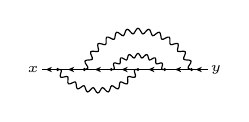
\begin{tikzpicture}[x=0.340cm, y=0.340cm, line width=0.420pt, baseline={([yshift=-0.6ex]0,0)}]
  \draw (-1.500,0.000) -- (-2.500,0.000);
  \fill (-2.119,0.000) -- (-1.881,-0.102) -- (-1.958,0.000) -- (-1.881,0.102) -- cycle;
  \draw (2.500,0.000) -- (1.500,0.000);
  \fill (1.881,0.000) -- (2.119,-0.102) -- (2.042,0.000) -- (2.119,0.102) -- cycle;
  \draw (-0.500,0.000) -- (-1.500,0.000);
  \fill (-1.119,0.000) -- (-0.881,-0.102) -- (-0.958,0.000) -- (-0.881,0.102) -- cycle;
  \draw (1.500,0.000) -- (0.500,0.000);
  \fill (0.881,0.000) -- (1.119,-0.102) -- (1.042,0.000) -- (1.119,0.102) -- cycle;
  \draw (0.500,0.000) -- (-0.500,0.000);
  \fill (-0.119,0.000) -- (0.119,-0.102) -- (0.042,0.000) -- (0.119,0.102) -- cycle;
  \draw plot[smooth, tension=0.7] coordinates {(-2.500,0.000) (-2.418,0.003) (-2.369,-0.015) (-2.364,-0.067) (-2.386,-0.146) (-2.406,-0.226) (-2.394,-0.281) (-2.340,-0.295) (-2.259,-0.279) (-2.179,-0.260) (-2.127,-0.268) (-2.111,-0.318) (-2.118,-0.399) (-2.121,-0.482) (-2.098,-0.533) (-2.042,-0.537) (-1.966,-0.505) (-1.892,-0.470) (-1.840,-0.467) (-1.814,-0.513) (-1.804,-0.594) (-1.791,-0.676) (-1.758,-0.721) (-1.702,-0.713) (-1.634,-0.667) (-1.569,-0.618) (-1.518,-0.605) (-1.484,-0.644) (-1.458,-0.722) (-1.428,-0.799) (-1.387,-0.837) (-1.334,-0.818) (-1.276,-0.759) (-1.222,-0.698) (-1.175,-0.675) (-1.133,-0.707) (-1.092,-0.778) (-1.048,-0.847) (-1.000,-0.876) (-0.952,-0.847) (-0.908,-0.778) (-0.867,-0.707) (-0.825,-0.675) (-0.778,-0.698) (-0.724,-0.759) (-0.666,-0.818) (-0.613,-0.837) (-0.572,-0.799) (-0.542,-0.722) (-0.516,-0.644) (-0.482,-0.605) (-0.431,-0.618) (-0.366,-0.667) (-0.298,-0.713) (-0.242,-0.721) (-0.209,-0.676) (-0.196,-0.594) (-0.186,-0.513) (-0.160,-0.467) (-0.108,-0.470) (-0.034,-0.505) (0.042,-0.537) (0.098,-0.533) (0.121,-0.482) (0.118,-0.399) (0.111,-0.318) (0.127,-0.268) (0.179,-0.260) (0.259,-0.279) (0.340,-0.295) (0.394,-0.281) (0.406,-0.226) (0.386,-0.146) (0.364,-0.067) (0.369,-0.015) (0.418,0.003) (0.500,0.000)};
  \draw plot[smooth, tension=0.7] coordinates {(2.500,0.000) (2.417,0.022) (2.372,0.055) (2.383,0.110) (2.430,0.182) (2.474,0.257) (2.479,0.315) (2.430,0.347) (2.343,0.356) (2.257,0.362) (2.207,0.387) (2.207,0.442) (2.240,0.522) (2.271,0.604) (2.264,0.662) (2.210,0.684) (2.123,0.678) (2.037,0.668) (1.984,0.683) (1.974,0.737) (1.992,0.822) (2.006,0.908) (1.990,0.964) (1.932,0.976) (1.848,0.953) (1.765,0.928) (1.710,0.933) (1.690,0.984) (1.692,1.071) (1.691,1.158) (1.664,1.210) (1.605,1.211) (1.527,1.173) (1.450,1.133) (1.395,1.128) (1.366,1.175) (1.352,1.260) (1.335,1.346) (1.299,1.392) (1.241,1.382) (1.171,1.331) (1.103,1.277) (1.050,1.262) (1.012,1.303) (0.983,1.384) (0.950,1.465) (0.906,1.504) (0.851,1.483) (0.792,1.420) (0.735,1.355) (0.685,1.330) (0.641,1.363) (0.597,1.438) (0.550,1.511) (0.500,1.541) (0.450,1.511) (0.403,1.438) (0.359,1.363) (0.315,1.330) (0.265,1.355) (0.208,1.420) (0.149,1.483) (0.094,1.504) (0.050,1.465) (0.017,1.384) (-0.012,1.303) (-0.050,1.262) (-0.103,1.277) (-0.171,1.331) (-0.241,1.382) (-0.299,1.392) (-0.335,1.346) (-0.352,1.260) (-0.366,1.175) (-0.395,1.128) (-0.450,1.133) (-0.527,1.173) (-0.605,1.211) (-0.664,1.210) (-0.691,1.158) (-0.692,1.071) (-0.690,0.984) (-0.710,0.933) (-0.765,0.928) (-0.848,0.953) (-0.932,0.976) (-0.990,0.964) (-1.006,0.908) (-0.992,0.822) (-0.974,0.737) (-0.984,0.683) (-1.037,0.668) (-1.123,0.678) (-1.210,0.684) (-1.264,0.662) (-1.271,0.604) (-1.240,0.522) (-1.207,0.442) (-1.207,0.387) (-1.257,0.362) (-1.343,0.356) (-1.430,0.347) (-1.479,0.315) (-1.474,0.257) (-1.430,0.182) (-1.383,0.110) (-1.372,0.055) (-1.417,0.022) (-1.500,0.000)};
  \draw plot[smooth, tension=0.7] coordinates {(1.500,0.000) (1.431,-0.003) (1.390,0.012) (1.385,0.055) (1.402,0.122) (1.417,0.190) (1.404,0.236) (1.358,0.247) (1.290,0.230) (1.224,0.210) (1.180,0.214) (1.164,0.254) (1.165,0.323) (1.161,0.393) (1.138,0.434) (1.090,0.433) (1.029,0.400) (0.970,0.363) (0.927,0.356) (0.901,0.391) (0.884,0.458) (0.863,0.525) (0.830,0.559) (0.784,0.546) (0.733,0.498) (0.685,0.448) (0.645,0.429) (0.611,0.457) (0.578,0.518) (0.541,0.577) (0.500,0.601) (0.459,0.577) (0.422,0.518) (0.389,0.457) (0.355,0.429) (0.315,0.448) (0.267,0.498) (0.216,0.546) (0.170,0.559) (0.137,0.525) (0.116,0.458) (0.099,0.391) (0.073,0.356) (0.030,0.363) (-0.029,0.400) (-0.090,0.433) (-0.138,0.434) (-0.161,0.393) (-0.165,0.323) (-0.164,0.254) (-0.180,0.214) (-0.224,0.210) (-0.290,0.230) (-0.358,0.247) (-0.404,0.236) (-0.417,0.190) (-0.402,0.122) (-0.385,0.055) (-0.390,0.012) (-0.431,-0.003) (-0.500,0.000)};
  \draw (-2.500,0.000) -- (-3.100,0.000);
  \fill (-2.949,0.000) -- (-2.711,-0.102) -- (-2.788,0.000) -- (-2.711,0.102) -- cycle;
  \draw (2.500,0.000) -- (3.100,0.000);
  \fill (2.651,0.000) -- (2.889,-0.102) -- (2.812,0.000) -- (2.889,0.102) -- cycle;
  \fill (-2.500,0.000) circle (0.064);
  \fill (2.500,0.000) circle (0.064);
  \fill (1.500,0.000) circle (0.064);
  \fill (-1.500,0.000) circle (0.064);
  \fill (0.500,0.000) circle (0.064);
  \fill (-0.500,0.000) circle (0.064);
  \node[font=\tiny, inner sep=0pt, anchor=0] at (-3.190,0.000) {$x$};
  \node[font=\tiny, inner sep=0pt, anchor=180] at (3.190,0.000) {$y$};
\end{tikzpicture}}
\diagramgap
\mbox{$\displaystyle -\,$\,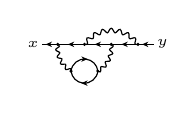
\begin{tikzpicture}[x=0.340cm, y=0.340cm, line width=0.420pt, baseline={([yshift=-0.6ex]0,0)}]
  \draw (-0.500,0.000) -- (-1.500,0.000);
  \fill (-1.119,0.000) -- (-0.881,-0.102) -- (-0.958,0.000) -- (-0.881,0.102) -- cycle;
  \draw (1.500,0.000) -- (0.500,0.000);
  \fill (0.881,0.000) -- (1.119,-0.102) -- (1.042,0.000) -- (1.119,0.102) -- cycle;
  \draw (0.500,0.000) -- (-0.500,0.000);
  \fill (-0.119,0.000) -- (0.119,-0.102) -- (0.042,0.000) -- (0.119,0.102) -- cycle;
  \draw (0.000,-1.000) arc[start angle=353.974, end angle=186.026, radius=0.503];
  \fill (-0.619,-1.450) -- (-0.381,-1.552) -- (-0.458,-1.450) -- (-0.381,-1.348) -- cycle;
  \draw (-1.000,-1.000) arc[start angle=173.974, end angle=6.026, radius=0.503];
  \fill (-0.381,-0.550) -- (-0.619,-0.448) -- (-0.542,-0.550) -- (-0.619,-0.652) -- cycle;
  \draw plot[smooth, tension=0.7] coordinates {(-1.500,0.000) (-1.455,-0.037) (-1.438,-0.070) (-1.459,-0.100) (-1.508,-0.131) (-1.556,-0.166) (-1.574,-0.202) (-1.551,-0.235) (-1.499,-0.263) (-1.447,-0.287) (-1.421,-0.314) (-1.434,-0.349) (-1.473,-0.392) (-1.510,-0.438) (-1.519,-0.477) (-1.488,-0.503) (-1.430,-0.517) (-1.373,-0.526) (-1.341,-0.546) (-1.345,-0.583) (-1.371,-0.634) (-1.395,-0.688) (-1.393,-0.729) (-1.357,-0.746) (-1.298,-0.743) (-1.240,-0.738) (-1.204,-0.748) (-1.198,-0.785) (-1.210,-0.842) (-1.219,-0.900) (-1.206,-0.938) (-1.167,-0.945) (-1.110,-0.928) (-1.056,-0.908) (-1.019,-0.908) (-1.003,-0.942) (-1.000,-1.000)};
  \draw plot[smooth, tension=0.7] coordinates {(1.500,0.000) (1.431,-0.003) (1.390,0.012) (1.385,0.055) (1.402,0.122) (1.417,0.190) (1.404,0.236) (1.358,0.247) (1.290,0.230) (1.224,0.210) (1.180,0.214) (1.164,0.254) (1.165,0.323) (1.161,0.393) (1.138,0.434) (1.090,0.433) (1.029,0.400) (0.970,0.363) (0.927,0.356) (0.901,0.391) (0.884,0.458) (0.863,0.525) (0.830,0.559) (0.784,0.546) (0.733,0.498) (0.685,0.448) (0.645,0.429) (0.611,0.457) (0.578,0.518) (0.541,0.577) (0.500,0.601) (0.459,0.577) (0.422,0.518) (0.389,0.457) (0.355,0.429) (0.315,0.448) (0.267,0.498) (0.216,0.546) (0.170,0.559) (0.137,0.525) (0.116,0.458) (0.099,0.391) (0.073,0.356) (0.030,0.363) (-0.029,0.400) (-0.090,0.433) (-0.138,0.434) (-0.161,0.393) (-0.165,0.323) (-0.164,0.254) (-0.180,0.214) (-0.224,0.210) (-0.290,0.230) (-0.358,0.247) (-0.404,0.236) (-0.417,0.190) (-0.402,0.122) (-0.385,0.055) (-0.390,0.012) (-0.431,-0.003) (-0.500,0.000)};
  \draw plot[smooth, tension=0.7] coordinates {(0.500,0.000) (0.552,-0.028) (0.575,-0.061) (0.556,-0.097) (0.508,-0.131) (0.459,-0.163) (0.438,-0.193) (0.455,-0.225) (0.499,-0.263) (0.542,-0.304) (0.556,-0.341) (0.529,-0.371) (0.473,-0.392) (0.418,-0.409) (0.389,-0.433) (0.397,-0.469) (0.430,-0.517) (0.461,-0.567) (0.464,-0.607) (0.430,-0.629) (0.371,-0.634) (0.313,-0.637) (0.280,-0.652) (0.278,-0.689) (0.298,-0.743) (0.314,-0.800) (0.307,-0.840) (0.268,-0.852) (0.210,-0.842) (0.153,-0.829) (0.117,-0.835) (0.106,-0.870) (0.110,-0.928) (0.111,-0.987) (0.094,-1.023) (0.054,-1.025) (0.000,-1.000)};
  \draw (-1.500,0.000) -- (-2.100,0.000);
  \fill (-1.949,0.000) -- (-1.711,-0.102) -- (-1.788,0.000) -- (-1.711,0.102) -- cycle;
  \draw (1.500,0.000) -- (2.100,0.000);
  \fill (1.651,0.000) -- (1.889,-0.102) -- (1.812,0.000) -- (1.889,0.102) -- cycle;
  \fill (-1.500,0.000) circle (0.064);
  \fill (1.500,0.000) circle (0.064);
  \fill (0.500,0.000) circle (0.064);
  \fill (-0.500,0.000) circle (0.064);
  \fill (-1.000,-1.000) circle (0.064);
  \fill (0.000,-1.000) circle (0.064);
  \node[font=\tiny, inner sep=0pt, anchor=0] at (-2.190,0.000) {$x$};
  \node[font=\tiny, inner sep=0pt, anchor=180] at (2.190,0.000) {$y$};
\end{tikzpicture}}
\diagramgap
\mbox{$\displaystyle -\,$\,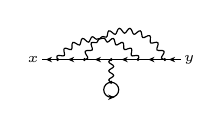
\begin{tikzpicture}[x=0.340cm, y=0.340cm, line width=0.420pt, baseline={([yshift=-0.6ex]0,0)}]
  \draw (-1.000,0.000) -- (-2.000,0.000);
  \fill (-1.619,0.000) -- (-1.381,-0.102) -- (-1.458,0.000) -- (-1.381,0.102) -- cycle;
  \draw (2.000,0.000) -- (1.000,0.000);
  \fill (1.381,0.000) -- (1.619,-0.102) -- (1.542,0.000) -- (1.619,0.102) -- cycle;
  \draw (0.000,0.000) -- (-1.000,0.000);
  \fill (-0.619,0.000) -- (-0.381,-0.102) -- (-0.458,0.000) -- (-0.381,0.102) -- cycle;
  \draw (1.000,0.000) -- (0.000,0.000);
  \fill (0.381,0.000) -- (0.619,-0.102) -- (0.542,0.000) -- (0.619,0.102) -- cycle;
  \draw plot[smooth, tension=0.7] coordinates {(-2.000,0.000) (-2.028,0.078) (-2.021,0.133) (-1.969,0.154) (-1.886,0.146) (-1.805,0.135) (-1.755,0.148) (-1.744,0.199) (-1.759,0.279) (-1.770,0.361) (-1.752,0.414) (-1.697,0.424) (-1.618,0.399) (-1.541,0.372) (-1.488,0.375) (-1.468,0.423) (-1.466,0.505) (-1.461,0.587) (-1.433,0.636) (-1.377,0.634) (-1.304,0.594) (-1.234,0.552) (-1.182,0.544) (-1.152,0.587) (-1.134,0.667) (-1.112,0.747) (-1.075,0.788) (-1.021,0.775) (-0.958,0.722) (-0.897,0.667) (-0.848,0.649) (-0.810,0.685) (-0.776,0.759) (-0.739,0.831) (-0.693,0.853) (-0.642,0.821) (-0.592,0.778) (-0.546,0.760) (-0.500,0.769) (-0.454,0.778) (-0.408,0.778) (-0.361,0.782) (-0.313,0.797) (-0.265,0.797) (-0.224,0.759) (-0.188,0.694) (-0.151,0.651) (-0.103,0.667) (-0.042,0.722) (0.021,0.775) (0.075,0.788) (0.112,0.747) (0.134,0.667) (0.152,0.587) (0.182,0.544) (0.234,0.552) (0.304,0.594) (0.377,0.634) (0.433,0.636) (0.461,0.587) (0.466,0.505) (0.468,0.423) (0.488,0.375) (0.541,0.372) (0.618,0.399) (0.697,0.424) (0.752,0.414) (0.770,0.361) (0.759,0.279) (0.744,0.199) (0.755,0.148) (0.805,0.135) (0.886,0.146) (0.969,0.154) (1.021,0.133) (1.028,0.078) (1.000,0.000)};
  \draw plot[smooth, tension=0.7] coordinates {(2.000,0.000) (1.920,0.020) (1.877,0.052) (1.886,0.104) (1.930,0.174) (1.971,0.248) (1.973,0.305) (1.924,0.334) (1.840,0.339) (1.757,0.340) (1.708,0.360) (1.704,0.413) (1.731,0.492) (1.753,0.573) (1.742,0.629) (1.687,0.646) (1.604,0.631) (1.523,0.612) (1.471,0.621) (1.455,0.671) (1.462,0.754) (1.465,0.838) (1.440,0.890) (1.383,0.893) (1.306,0.859) (1.232,0.822) (1.179,0.818) (1.152,0.863) (1.139,0.945) (1.122,1.027) (1.086,1.072) (1.030,1.062) (0.963,1.011) (0.900,0.957) (0.849,0.941) (0.812,0.978) (0.781,1.055) (0.744,1.131) (0.699,1.166) (0.647,1.143) (0.594,1.077) (0.545,1.010) (0.500,0.982) (0.455,1.010) (0.406,1.077) (0.353,1.143) (0.301,1.166) (0.256,1.131) (0.219,1.055) (0.188,0.978) (0.151,0.941) (0.100,0.957) (0.037,1.011) (-0.030,1.062) (-0.086,1.072) (-0.122,1.027) (-0.139,0.945) (-0.154,0.867) (-0.188,0.835) (-0.245,0.845) (-0.306,0.859) (-0.354,0.847) (-0.389,0.814) (-0.424,0.782) (-0.462,0.754) (-0.492,0.716) (-0.513,0.669) (-0.544,0.635) (-0.604,0.631) (-0.682,0.641) (-0.741,0.629) (-0.753,0.573) (-0.731,0.492) (-0.704,0.413) (-0.708,0.360) (-0.757,0.340) (-0.840,0.339) (-0.924,0.334) (-0.973,0.305) (-0.971,0.248) (-0.930,0.174) (-0.886,0.104) (-0.877,0.052) (-0.920,0.020) (-1.000,0.000)};
  \draw plot[smooth, tension=0.7] coordinates {(0.000,-0.850) (-0.065,-0.808) (-0.092,-0.765) (-0.065,-0.722) (0.000,-0.680) (0.065,-0.638) (0.092,-0.595) (0.065,-0.552) (0.000,-0.510) (-0.065,-0.467) (-0.092,-0.425) (-0.065,-0.382) (0.000,-0.340) (0.065,-0.298) (0.092,-0.255) (0.065,-0.213) (0.000,-0.170) (-0.065,-0.127) (-0.092,-0.085) (-0.065,-0.042) (0.000,0.000)};
  \draw (0.000,-0.850) arc[start angle=90.000, end angle=450.000, radius=0.280];
  \fill (0.119,-1.410) -- (-0.119,-1.308) -- (-0.042,-1.410) -- (-0.119,-1.512) -- cycle;
  \draw (-2.000,0.000) -- (-2.600,0.000);
  \fill (-2.449,0.000) -- (-2.211,-0.102) -- (-2.288,0.000) -- (-2.211,0.102) -- cycle;
  \draw (2.000,0.000) -- (2.600,0.000);
  \fill (2.151,0.000) -- (2.389,-0.102) -- (2.312,0.000) -- (2.389,0.102) -- cycle;
  \fill (-2.000,0.000) circle (0.064);
  \fill (2.000,0.000) circle (0.064);
  \fill (0.000,-0.850) circle (0.064);
  \fill (1.000,0.000) circle (0.064);
  \fill (-1.000,0.000) circle (0.064);
  \fill (0.000,0.000) circle (0.064);
  \node[font=\tiny, inner sep=0pt, anchor=0] at (-2.690,0.000) {$x$};
  \node[font=\tiny, inner sep=0pt, anchor=180] at (2.690,0.000) {$y$};
\end{tikzpicture}}
\diagramgap
\mbox{$\displaystyle -\,$\,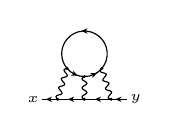
\begin{tikzpicture}[x=0.340cm, y=0.340cm, line width=0.420pt, baseline={([yshift=-0.6ex]0,0)}]
  \draw (0.000,0.000) -- (-1.000,0.000);
  \fill (-0.619,0.000) -- (-0.381,-0.102) -- (-0.458,0.000) -- (-0.381,0.102) -- cycle;
  \draw (1.000,0.000) -- (0.000,0.000);
  \fill (0.381,0.000) -- (0.619,-0.102) -- (0.542,0.000) -- (0.619,0.102) -- cycle;
  \draw (0.651,1.154) arc[start angle=320.000, end angle=580.000, radius=0.850];
  \fill (-0.119,2.550) -- (0.119,2.448) -- (0.042,2.550) -- (0.119,2.652) -- cycle;
  \draw (0.000,0.850) arc[start angle=270.000, end angle=320.000, radius=0.850];
  \fill (0.467,0.980) -- (0.208,0.972) -- (0.321,0.912) -- (0.294,0.787) -- cycle;
  \draw (-0.651,1.154) arc[start angle=220.000, end angle=270.000, radius=0.850];
  \fill (-0.251,0.879) -- (-0.424,1.073) -- (-0.397,0.947) -- (-0.511,0.888) -- cycle;
  \draw plot[smooth, tension=0.7] coordinates {(-1.000,0.000) (-1.050,0.060) (-1.064,0.109) (-1.026,0.143) (-0.950,0.165) (-0.875,0.187) (-0.836,0.220) (-0.850,0.269) (-0.900,0.330) (-0.951,0.390) (-0.964,0.439) (-0.926,0.472) (-0.850,0.494) (-0.775,0.517) (-0.737,0.550) (-0.750,0.599) (-0.801,0.659) (-0.851,0.719) (-0.865,0.769) (-0.826,0.802) (-0.751,0.824) (-0.675,0.846) (-0.637,0.880) (-0.651,0.929) (-0.701,0.989) (-0.751,1.049) (-0.765,1.098) (-0.727,1.131) (-0.651,1.154)};
  \draw plot[smooth, tension=0.7] coordinates {(1.000,0.000) (0.925,0.022) (0.886,0.055) (0.900,0.105) (0.950,0.165) (1.001,0.225) (1.014,0.274) (0.976,0.307) (0.900,0.330) (0.825,0.352) (0.786,0.385) (0.800,0.434) (0.850,0.494) (0.901,0.555) (0.915,0.604) (0.876,0.637) (0.801,0.659) (0.725,0.681) (0.687,0.715) (0.700,0.764) (0.751,0.824) (0.801,0.884) (0.815,0.933) (0.776,0.967) (0.701,0.989) (0.626,1.011) (0.587,1.044) (0.601,1.093) (0.651,1.154)};
  \draw plot[smooth, tension=0.7] coordinates {(0.000,0.000) (-0.065,0.042) (-0.092,0.085) (-0.065,0.128) (0.000,0.170) (0.065,0.212) (0.092,0.255) (0.065,0.298) (0.000,0.340) (-0.065,0.382) (-0.092,0.425) (-0.065,0.468) (0.000,0.510) (0.065,0.552) (0.092,0.595) (0.065,0.638) (0.000,0.680) (-0.065,0.722) (-0.092,0.765) (-0.065,0.808) (0.000,0.850)};
  \draw (-1.000,0.000) -- (-1.600,0.000);
  \fill (-1.449,0.000) -- (-1.211,-0.102) -- (-1.288,0.000) -- (-1.211,0.102) -- cycle;
  \draw (1.000,0.000) -- (1.600,0.000);
  \fill (1.151,0.000) -- (1.389,-0.102) -- (1.312,0.000) -- (1.389,0.102) -- cycle;
  \fill (-1.000,0.000) circle (0.064);
  \fill (1.000,0.000) circle (0.064);
  \fill (0.000,0.000) circle (0.064);
  \fill (-0.651,1.154) circle (0.064);
  \fill (0.651,1.154) circle (0.064);
  \fill (0.000,0.850) circle (0.064);
  \node[font=\tiny, inner sep=0pt, anchor=0] at (-1.690,0.000) {$x$};
  \node[font=\tiny, inner sep=0pt, anchor=180] at (1.690,0.000) {$y$};
\end{tikzpicture}}
\diagramgap
\mbox{$\displaystyle +\,$\,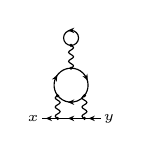
\begin{tikzpicture}[x=0.340cm, y=0.340cm, line width=0.420pt, baseline={([yshift=-0.6ex]0,0)}]
  \draw (0.500,0.000) -- (-0.500,0.000);
  \fill (-0.119,0.000) -- (0.119,-0.102) -- (0.042,0.000) -- (0.119,0.102) -- cycle;
  \draw (0.500,0.850) arc[start angle=321.934, end angle=218.066, radius=0.635];
  \fill (-0.119,0.606) -- (0.119,0.504) -- (0.042,0.606) -- (0.119,0.709) -- cycle;
  \draw (0.000,1.877) arc[start angle=90.000, end angle=-38.066, radius=0.635];
  \fill (0.623,1.412) -- (0.610,1.672) -- (0.553,1.557) -- (0.427,1.582) -- cycle;
  \draw (-0.500,0.850) arc[start angle=218.066, end angle=90.000, radius=0.635];
  \fill (-0.519,1.627) -- (-0.715,1.457) -- (-0.589,1.482) -- (-0.532,1.368) -- cycle;
  \draw plot[smooth, tension=0.7] coordinates {(-0.500,0.000) (-0.565,0.043) (-0.592,0.085) (-0.565,0.128) (-0.500,0.170) (-0.435,0.213) (-0.408,0.255) (-0.435,0.298) (-0.500,0.340) (-0.565,0.383) (-0.592,0.425) (-0.565,0.468) (-0.500,0.510) (-0.435,0.553) (-0.408,0.595) (-0.435,0.638) (-0.500,0.680) (-0.565,0.723) (-0.592,0.765) (-0.565,0.808) (-0.500,0.850)};
  \draw plot[smooth, tension=0.7] coordinates {(0.500,0.000) (0.435,0.042) (0.408,0.085) (0.435,0.127) (0.500,0.170) (0.565,0.212) (0.592,0.255) (0.565,0.298) (0.500,0.340) (0.435,0.382) (0.408,0.425) (0.435,0.467) (0.500,0.510) (0.565,0.552) (0.592,0.595) (0.565,0.638) (0.500,0.680) (0.435,0.722) (0.408,0.765) (0.435,0.807) (0.500,0.850)};
  \draw plot[smooth, tension=0.7] coordinates {(0.000,2.727) (0.065,2.684) (0.092,2.642) (0.065,2.599) (0.000,2.557) (-0.065,2.514) (-0.092,2.472) (-0.065,2.429) (0.000,2.387) (0.065,2.344) (0.092,2.302) (0.065,2.259) (0.000,2.217) (-0.065,2.174) (-0.092,2.132) (-0.065,2.089) (0.000,2.047) (0.065,2.004) (0.092,1.962) (0.065,1.919) (0.000,1.877)};
  \draw (0.000,2.727) arc[start angle=270.000, end angle=630.000, radius=0.280];
  \fill (-0.119,3.287) -- (0.119,3.185) -- (0.042,3.287) -- (0.119,3.389) -- cycle;
  \draw (-0.500,0.000) -- (-1.100,0.000);
  \fill (-0.949,0.000) -- (-0.711,-0.102) -- (-0.788,0.000) -- (-0.711,0.102) -- cycle;
  \draw (0.500,0.000) -- (1.100,0.000);
  \fill (0.651,0.000) -- (0.889,-0.102) -- (0.812,0.000) -- (0.889,0.102) -- cycle;
  \fill (-0.500,0.000) circle (0.064);
  \fill (0.500,0.000) circle (0.064);
  \fill (0.000,2.727) circle (0.064);
  \fill (-0.500,0.850) circle (0.064);
  \fill (0.500,0.850) circle (0.064);
  \fill (0.000,1.877) circle (0.064);
  \node[font=\tiny, inner sep=0pt, anchor=0] at (-1.190,0.000) {$x$};
  \node[font=\tiny, inner sep=0pt, anchor=180] at (1.190,0.000) {$y$};
\end{tikzpicture}}
\diagramgap
\mbox{$\displaystyle -\,$\,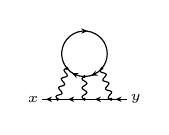
\begin{tikzpicture}[x=0.340cm, y=0.340cm, line width=0.420pt, baseline={([yshift=-0.6ex]0,0)}]
  \draw (0.000,0.000) -- (-1.000,0.000);
  \fill (-0.619,0.000) -- (-0.381,-0.102) -- (-0.458,0.000) -- (-0.381,0.102) -- cycle;
  \draw (1.000,0.000) -- (0.000,0.000);
  \fill (0.381,0.000) -- (0.619,-0.102) -- (0.542,0.000) -- (0.619,0.102) -- cycle;
  \draw (0.000,0.850) arc[start angle=270.000, end angle=220.000, radius=0.850];
  \fill (-0.467,0.980) -- (-0.294,0.787) -- (-0.321,0.912) -- (-0.208,0.972) -- cycle;
  \draw (-0.651,1.154) arc[start angle=220.000, end angle=-40.000, radius=0.850];
  \fill (0.119,2.550) -- (-0.119,2.652) -- (-0.042,2.550) -- (-0.119,2.448) -- cycle;
  \draw (0.651,1.154) arc[start angle=320.000, end angle=270.000, radius=0.850];
  \fill (0.251,0.879) -- (0.511,0.888) -- (0.397,0.947) -- (0.424,1.073) -- cycle;
  \draw plot[smooth, tension=0.7] coordinates {(-1.000,0.000) (-1.050,0.060) (-1.064,0.109) (-1.026,0.143) (-0.950,0.165) (-0.875,0.187) (-0.836,0.220) (-0.850,0.269) (-0.900,0.330) (-0.951,0.390) (-0.964,0.439) (-0.926,0.472) (-0.850,0.494) (-0.775,0.517) (-0.737,0.550) (-0.750,0.599) (-0.801,0.659) (-0.851,0.719) (-0.865,0.769) (-0.826,0.802) (-0.751,0.824) (-0.675,0.846) (-0.637,0.880) (-0.651,0.929) (-0.701,0.989) (-0.751,1.049) (-0.765,1.098) (-0.727,1.131) (-0.651,1.154)};
  \draw plot[smooth, tension=0.7] coordinates {(1.000,0.000) (0.925,0.022) (0.886,0.055) (0.900,0.105) (0.950,0.165) (1.001,0.225) (1.014,0.274) (0.976,0.307) (0.900,0.330) (0.825,0.352) (0.786,0.385) (0.800,0.434) (0.850,0.494) (0.901,0.555) (0.915,0.604) (0.876,0.637) (0.801,0.659) (0.725,0.681) (0.687,0.715) (0.700,0.764) (0.751,0.824) (0.801,0.884) (0.815,0.933) (0.776,0.967) (0.701,0.989) (0.626,1.011) (0.587,1.044) (0.601,1.093) (0.651,1.154)};
  \draw plot[smooth, tension=0.7] coordinates {(0.000,0.000) (-0.065,0.042) (-0.092,0.085) (-0.065,0.128) (0.000,0.170) (0.065,0.212) (0.092,0.255) (0.065,0.298) (0.000,0.340) (-0.065,0.382) (-0.092,0.425) (-0.065,0.468) (0.000,0.510) (0.065,0.552) (0.092,0.595) (0.065,0.638) (0.000,0.680) (-0.065,0.722) (-0.092,0.765) (-0.065,0.808) (0.000,0.850)};
  \draw (-1.000,0.000) -- (-1.600,0.000);
  \fill (-1.449,0.000) -- (-1.211,-0.102) -- (-1.288,0.000) -- (-1.211,0.102) -- cycle;
  \draw (1.000,0.000) -- (1.600,0.000);
  \fill (1.151,0.000) -- (1.389,-0.102) -- (1.312,0.000) -- (1.389,0.102) -- cycle;
  \fill (-1.000,0.000) circle (0.064);
  \fill (1.000,0.000) circle (0.064);
  \fill (0.000,0.000) circle (0.064);
  \fill (-0.651,1.154) circle (0.064);
  \fill (0.651,1.154) circle (0.064);
  \fill (0.000,0.850) circle (0.064);
  \node[font=\tiny, inner sep=0pt, anchor=0] at (-1.690,0.000) {$x$};
  \node[font=\tiny, inner sep=0pt, anchor=180] at (1.690,0.000) {$y$};
\end{tikzpicture}}
\diagramgap
\mbox{$\displaystyle +\,$\,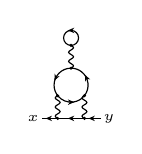
\begin{tikzpicture}[x=0.340cm, y=0.340cm, line width=0.420pt, baseline={([yshift=-0.6ex]0,0)}]
  \draw (0.500,0.000) -- (-0.500,0.000);
  \fill (-0.119,0.000) -- (0.119,-0.102) -- (0.042,0.000) -- (0.119,0.102) -- cycle;
  \draw (0.000,1.877) arc[start angle=90.000, end angle=218.066, radius=0.635];
  \fill (-0.623,1.412) -- (-0.427,1.582) -- (-0.553,1.557) -- (-0.610,1.672) -- cycle;
  \draw (-0.500,0.850) arc[start angle=218.066, end angle=321.934, radius=0.635];
  \fill (0.119,0.606) -- (-0.119,0.709) -- (-0.042,0.606) -- (-0.119,0.504) -- cycle;
  \draw (0.500,0.850) arc[start angle=321.934, end angle=450.000, radius=0.635];
  \fill (0.519,1.627) -- (0.532,1.368) -- (0.589,1.482) -- (0.715,1.457) -- cycle;
  \draw plot[smooth, tension=0.7] coordinates {(-0.500,0.000) (-0.565,0.043) (-0.592,0.085) (-0.565,0.128) (-0.500,0.170) (-0.435,0.213) (-0.408,0.255) (-0.435,0.298) (-0.500,0.340) (-0.565,0.383) (-0.592,0.425) (-0.565,0.468) (-0.500,0.510) (-0.435,0.553) (-0.408,0.595) (-0.435,0.638) (-0.500,0.680) (-0.565,0.723) (-0.592,0.765) (-0.565,0.808) (-0.500,0.850)};
  \draw plot[smooth, tension=0.7] coordinates {(0.500,0.000) (0.435,0.042) (0.408,0.085) (0.435,0.127) (0.500,0.170) (0.565,0.212) (0.592,0.255) (0.565,0.298) (0.500,0.340) (0.435,0.382) (0.408,0.425) (0.435,0.467) (0.500,0.510) (0.565,0.552) (0.592,0.595) (0.565,0.638) (0.500,0.680) (0.435,0.722) (0.408,0.765) (0.435,0.807) (0.500,0.850)};
  \draw plot[smooth, tension=0.7] coordinates {(0.000,2.727) (0.065,2.684) (0.092,2.642) (0.065,2.599) (0.000,2.557) (-0.065,2.514) (-0.092,2.472) (-0.065,2.429) (0.000,2.387) (0.065,2.344) (0.092,2.302) (0.065,2.259) (0.000,2.217) (-0.065,2.174) (-0.092,2.132) (-0.065,2.089) (0.000,2.047) (0.065,2.004) (0.092,1.962) (0.065,1.919) (0.000,1.877)};
  \draw (0.000,2.727) arc[start angle=270.000, end angle=630.000, radius=0.280];
  \fill (-0.119,3.287) -- (0.119,3.185) -- (0.042,3.287) -- (0.119,3.389) -- cycle;
  \draw (-0.500,0.000) -- (-1.100,0.000);
  \fill (-0.949,0.000) -- (-0.711,-0.102) -- (-0.788,0.000) -- (-0.711,0.102) -- cycle;
  \draw (0.500,0.000) -- (1.100,0.000);
  \fill (0.651,0.000) -- (0.889,-0.102) -- (0.812,0.000) -- (0.889,0.102) -- cycle;
  \fill (-0.500,0.000) circle (0.064);
  \fill (0.500,0.000) circle (0.064);
  \fill (0.000,2.727) circle (0.064);
  \fill (-0.500,0.850) circle (0.064);
  \fill (0.500,0.850) circle (0.064);
  \fill (0.000,1.877) circle (0.064);
  \node[font=\tiny, inner sep=0pt, anchor=0] at (-1.190,0.000) {$x$};
  \node[font=\tiny, inner sep=0pt, anchor=180] at (1.190,0.000) {$y$};
\end{tikzpicture}}
\diagramgap
\mbox{$\displaystyle +\,$\,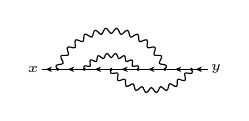
\begin{tikzpicture}[x=0.340cm, y=0.340cm, line width=0.420pt, baseline={([yshift=-0.6ex]0,0)}]
  \draw (-1.500,0.000) -- (-2.500,0.000);
  \fill (-2.119,0.000) -- (-1.881,-0.102) -- (-1.958,0.000) -- (-1.881,0.102) -- cycle;
  \draw (2.500,0.000) -- (1.500,0.000);
  \fill (1.881,0.000) -- (2.119,-0.102) -- (2.042,0.000) -- (2.119,0.102) -- cycle;
  \draw (-0.500,0.000) -- (-1.500,0.000);
  \fill (-1.119,0.000) -- (-0.881,-0.102) -- (-0.958,0.000) -- (-0.881,0.102) -- cycle;
  \draw (0.500,0.000) -- (-0.500,0.000);
  \fill (-0.119,0.000) -- (0.119,-0.102) -- (0.042,0.000) -- (0.119,0.102) -- cycle;
  \draw (1.500,0.000) -- (0.500,0.000);
  \fill (0.881,0.000) -- (1.119,-0.102) -- (1.042,0.000) -- (1.119,0.102) -- cycle;
  \draw plot[smooth, tension=0.7] coordinates {(-2.500,0.000) (-2.551,0.070) (-2.562,0.128) (-2.515,0.164) (-2.430,0.182) (-2.345,0.196) (-2.298,0.225) (-2.303,0.280) (-2.343,0.356) (-2.381,0.435) (-2.380,0.494) (-2.328,0.521) (-2.240,0.522) (-2.154,0.520) (-2.103,0.540) (-2.098,0.595) (-2.123,0.678) (-2.146,0.762) (-2.134,0.819) (-2.078,0.836) (-1.992,0.822) (-1.907,0.804) (-1.853,0.814) (-1.838,0.867) (-1.848,0.953) (-1.855,1.040) (-1.833,1.094) (-1.774,1.101) (-1.692,1.071) (-1.613,1.038) (-1.557,1.038) (-1.533,1.087) (-1.527,1.173) (-1.517,1.260) (-1.486,1.309) (-1.427,1.305) (-1.352,1.260) (-1.280,1.213) (-1.226,1.203) (-1.192,1.247) (-1.171,1.331) (-1.145,1.414) (-1.105,1.457) (-1.048,1.442) (-0.983,1.384) (-0.921,1.324) (-0.869,1.304) (-0.828,1.342) (-0.792,1.420) (-0.751,1.497) (-0.704,1.532) (-0.651,1.506) (-0.597,1.438) (-0.547,1.368) (-0.500,1.339) (-0.453,1.368) (-0.403,1.438) (-0.349,1.506) (-0.296,1.532) (-0.249,1.497) (-0.208,1.420) (-0.172,1.342) (-0.131,1.304) (-0.079,1.324) (-0.017,1.384) (0.048,1.442) (0.105,1.457) (0.145,1.414) (0.171,1.331) (0.192,1.247) (0.226,1.203) (0.280,1.213) (0.352,1.260) (0.427,1.305) (0.486,1.309) (0.517,1.260) (0.527,1.173) (0.533,1.087) (0.557,1.038) (0.613,1.038) (0.692,1.071) (0.774,1.101) (0.833,1.094) (0.855,1.040) (0.848,0.953) (0.838,0.867) (0.853,0.814) (0.907,0.804) (0.992,0.822) (1.078,0.836) (1.134,0.819) (1.146,0.762) (1.123,0.678) (1.098,0.595) (1.103,0.540) (1.154,0.520) (1.240,0.522) (1.328,0.521) (1.380,0.494) (1.381,0.435) (1.343,0.356) (1.303,0.280) (1.298,0.225) (1.345,0.196) (1.430,0.182) (1.515,0.164) (1.562,0.128) (1.551,0.070) (1.500,0.000)};
  \draw plot[smooth, tension=0.7] coordinates {(2.500,0.000) (2.528,-0.078) (2.521,-0.133) (2.469,-0.154) (2.386,-0.146) (2.305,-0.135) (2.255,-0.148) (2.244,-0.199) (2.259,-0.279) (2.270,-0.361) (2.252,-0.414) (2.197,-0.424) (2.118,-0.399) (2.041,-0.372) (1.988,-0.375) (1.968,-0.423) (1.966,-0.505) (1.961,-0.587) (1.933,-0.636) (1.877,-0.634) (1.804,-0.594) (1.734,-0.552) (1.682,-0.544) (1.652,-0.587) (1.634,-0.667) (1.612,-0.747) (1.575,-0.788) (1.521,-0.775) (1.458,-0.722) (1.397,-0.667) (1.348,-0.649) (1.310,-0.685) (1.276,-0.759) (1.239,-0.833) (1.194,-0.866) (1.144,-0.843) (1.092,-0.778) (1.045,-0.711) (1.000,-0.684) (0.955,-0.711) (0.908,-0.778) (0.856,-0.843) (0.806,-0.866) (0.761,-0.833) (0.724,-0.759) (0.690,-0.685) (0.652,-0.649) (0.603,-0.667) (0.542,-0.722) (0.479,-0.775) (0.425,-0.788) (0.388,-0.747) (0.366,-0.667) (0.348,-0.587) (0.318,-0.544) (0.266,-0.552) (0.196,-0.594) (0.123,-0.634) (0.067,-0.636) (0.039,-0.587) (0.034,-0.505) (0.032,-0.423) (0.012,-0.375) (-0.041,-0.372) (-0.118,-0.399) (-0.197,-0.424) (-0.252,-0.414) (-0.270,-0.361) (-0.259,-0.279) (-0.244,-0.199) (-0.255,-0.148) (-0.305,-0.135) (-0.386,-0.146) (-0.469,-0.154) (-0.521,-0.133) (-0.528,-0.078) (-0.500,0.000)};
  \draw plot[smooth, tension=0.7] coordinates {(-1.500,0.000) (-1.523,0.066) (-1.517,0.113) (-1.472,0.130) (-1.402,0.122) (-1.334,0.110) (-1.292,0.119) (-1.281,0.162) (-1.290,0.230) (-1.296,0.300) (-1.277,0.344) (-1.230,0.349) (-1.165,0.323) (-1.102,0.295) (-1.058,0.293) (-1.037,0.331) (-1.029,0.400) (-1.016,0.469) (-0.988,0.507) (-0.941,0.499) (-0.884,0.458) (-0.830,0.415) (-0.788,0.402) (-0.758,0.434) (-0.733,0.498) (-0.704,0.561) (-0.666,0.591) (-0.622,0.572) (-0.578,0.518) (-0.537,0.462) (-0.500,0.439) (-0.463,0.462) (-0.422,0.518) (-0.378,0.572) (-0.334,0.591) (-0.296,0.561) (-0.267,0.498) (-0.242,0.434) (-0.212,0.402) (-0.170,0.415) (-0.116,0.458) (-0.059,0.499) (-0.012,0.507) (0.016,0.469) (0.029,0.400) (0.037,0.331) (0.058,0.293) (0.102,0.295) (0.165,0.323) (0.230,0.349) (0.277,0.344) (0.296,0.300) (0.290,0.230) (0.281,0.162) (0.292,0.119) (0.334,0.110) (0.402,0.122) (0.472,0.130) (0.517,0.113) (0.523,0.066) (0.500,0.000)};
  \draw (-2.500,0.000) -- (-3.100,0.000);
  \fill (-2.949,0.000) -- (-2.711,-0.102) -- (-2.788,0.000) -- (-2.711,0.102) -- cycle;
  \draw (2.500,0.000) -- (3.100,0.000);
  \fill (2.651,0.000) -- (2.889,-0.102) -- (2.812,0.000) -- (2.889,0.102) -- cycle;
  \fill (-2.500,0.000) circle (0.064);
  \fill (2.500,0.000) circle (0.064);
  \fill (1.500,0.000) circle (0.064);
  \fill (-1.500,0.000) circle (0.064);
  \fill (-0.500,0.000) circle (0.064);
  \fill (0.500,0.000) circle (0.064);
  \node[font=\tiny, inner sep=0pt, anchor=0] at (-3.190,0.000) {$x$};
  \node[font=\tiny, inner sep=0pt, anchor=180] at (3.190,0.000) {$y$};
\end{tikzpicture}}
\diagramgap
\mbox{$\displaystyle +\,$\,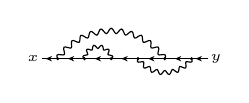
\begin{tikzpicture}[x=0.340cm, y=0.340cm, line width=0.420pt, baseline={([yshift=-0.6ex]0,0)}]
  \draw (-1.500,0.000) -- (-2.500,0.000);
  \fill (-2.119,0.000) -- (-1.881,-0.102) -- (-1.958,0.000) -- (-1.881,0.102) -- cycle;
  \draw (2.500,0.000) -- (1.500,0.000);
  \fill (1.881,0.000) -- (2.119,-0.102) -- (2.042,0.000) -- (2.119,0.102) -- cycle;
  \draw (-0.500,0.000) -- (-1.500,0.000);
  \fill (-1.119,0.000) -- (-0.881,-0.102) -- (-0.958,0.000) -- (-0.881,0.102) -- cycle;
  \draw plot[smooth, tension=0.7] coordinates {(-1.500,0.000) (-1.544,0.042) (-1.556,0.082) (-1.527,0.113) (-1.468,0.130) (-1.411,0.140) (-1.379,0.157) (-1.381,0.193) (-1.404,0.247) (-1.421,0.305) (-1.410,0.346) (-1.369,0.358) (-1.311,0.342) (-1.256,0.322) (-1.220,0.320) (-1.204,0.352) (-1.196,0.410) (-1.181,0.469) (-1.151,0.499) (-1.110,0.488) (-1.067,0.446) (-1.030,0.400) (-1.000,0.380) (-0.970,0.400) (-0.933,0.446) (-0.890,0.488) (-0.849,0.499) (-0.819,0.469) (-0.804,0.410) (-0.796,0.352) (-0.780,0.320) (-0.744,0.322) (-0.689,0.342) (-0.631,0.358) (-0.590,0.346) (-0.579,0.305) (-0.596,0.247) (-0.619,0.193) (-0.621,0.157) (-0.589,0.140) (-0.532,0.130) (-0.473,0.113) (-0.444,0.082) (-0.456,0.042) (-0.500,0.000)};
  \draw (1.500,0.000) -- (0.500,0.000);
  \fill (0.881,0.000) -- (1.119,-0.102) -- (1.042,0.000) -- (1.119,0.102) -- cycle;
  \draw (0.500,0.000) -- (-0.500,0.000);
  \fill (-0.119,0.000) -- (0.119,-0.102) -- (0.042,0.000) -- (0.119,0.102) -- cycle;
  \draw plot[smooth, tension=0.7] coordinates {(-2.500,0.000) (-2.528,0.079) (-2.522,0.135) (-2.470,0.155) (-2.387,0.149) (-2.304,0.140) (-2.253,0.156) (-2.244,0.208) (-2.262,0.289) (-2.278,0.371) (-2.264,0.426) (-2.209,0.438) (-2.127,0.419) (-2.047,0.398) (-1.994,0.405) (-1.977,0.456) (-1.983,0.539) (-1.986,0.622) (-1.963,0.674) (-1.907,0.678) (-1.829,0.647) (-1.754,0.613) (-1.700,0.612) (-1.675,0.660) (-1.668,0.742) (-1.659,0.826) (-1.629,0.873) (-1.573,0.868) (-1.501,0.826) (-1.431,0.781) (-1.378,0.772) (-1.346,0.815) (-1.327,0.896) (-1.305,0.977) (-1.267,1.019) (-1.213,1.006) (-1.148,0.952) (-1.086,0.898) (-1.035,0.881) (-0.997,0.918) (-0.966,0.995) (-0.931,1.072) (-0.888,1.108) (-0.836,1.086) (-0.781,1.024) (-0.727,0.960) (-0.680,0.936) (-0.637,0.967) (-0.594,1.038) (-0.548,1.108) (-0.500,1.137) (-0.452,1.108) (-0.406,1.038) (-0.363,0.967) (-0.320,0.936) (-0.273,0.960) (-0.219,1.024) (-0.164,1.086) (-0.112,1.108) (-0.069,1.072) (-0.034,0.995) (-0.003,0.918) (0.035,0.881) (0.086,0.898) (0.148,0.952) (0.213,1.006) (0.267,1.019) (0.305,0.977) (0.327,0.896) (0.346,0.815) (0.378,0.772) (0.431,0.781) (0.501,0.826) (0.573,0.868) (0.629,0.873) (0.659,0.826) (0.668,0.742) (0.675,0.660) (0.700,0.612) (0.754,0.613) (0.829,0.647) (0.907,0.678) (0.963,0.674) (0.986,0.622) (0.983,0.539) (0.977,0.456) (0.994,0.405) (1.047,0.398) (1.127,0.419) (1.209,0.438) (1.264,0.426) (1.278,0.371) (1.262,0.289) (1.244,0.208) (1.253,0.156) (1.304,0.140) (1.387,0.149) (1.470,0.155) (1.522,0.135) (1.528,0.079) (1.500,0.000)};
  \draw plot[smooth, tension=0.7] coordinates {(2.500,0.000) (2.523,-0.066) (2.517,-0.113) (2.472,-0.130) (2.402,-0.122) (2.334,-0.110) (2.292,-0.119) (2.281,-0.162) (2.290,-0.230) (2.296,-0.300) (2.277,-0.344) (2.230,-0.349) (2.165,-0.323) (2.102,-0.295) (2.058,-0.293) (2.037,-0.331) (2.029,-0.400) (2.016,-0.469) (1.988,-0.507) (1.941,-0.499) (1.884,-0.458) (1.830,-0.415) (1.788,-0.402) (1.758,-0.434) (1.733,-0.498) (1.704,-0.561) (1.666,-0.591) (1.622,-0.572) (1.578,-0.518) (1.537,-0.462) (1.500,-0.439) (1.463,-0.462) (1.422,-0.518) (1.378,-0.572) (1.334,-0.591) (1.296,-0.561) (1.267,-0.498) (1.242,-0.434) (1.212,-0.402) (1.170,-0.415) (1.116,-0.458) (1.059,-0.499) (1.012,-0.507) (0.984,-0.469) (0.971,-0.400) (0.963,-0.331) (0.942,-0.293) (0.898,-0.295) (0.835,-0.323) (0.770,-0.349) (0.723,-0.344) (0.704,-0.300) (0.710,-0.230) (0.719,-0.162) (0.708,-0.119) (0.666,-0.110) (0.598,-0.122) (0.528,-0.130) (0.483,-0.113) (0.477,-0.066) (0.500,0.000)};
  \draw (-2.500,0.000) -- (-3.100,0.000);
  \fill (-2.949,0.000) -- (-2.711,-0.102) -- (-2.788,0.000) -- (-2.711,0.102) -- cycle;
  \draw (2.500,0.000) -- (3.100,0.000);
  \fill (2.651,0.000) -- (2.889,-0.102) -- (2.812,0.000) -- (2.889,0.102) -- cycle;
  \fill (-2.500,0.000) circle (0.064);
  \fill (2.500,0.000) circle (0.064);
  \fill (1.500,0.000) circle (0.064);
  \fill (-1.500,0.000) circle (0.064);
  \fill (0.500,0.000) circle (0.064);
  \fill (-0.500,0.000) circle (0.064);
  \node[font=\tiny, inner sep=0pt, anchor=0] at (-3.190,0.000) {$x$};
  \node[font=\tiny, inner sep=0pt, anchor=180] at (3.190,0.000) {$y$};
\end{tikzpicture}}
\diagramgap
\mbox{$\displaystyle -\,$\,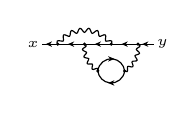
\begin{tikzpicture}[x=0.340cm, y=0.340cm, line width=0.420pt, baseline={([yshift=-0.6ex]0,0)}]
  \draw (-0.500,0.000) -- (-1.500,0.000);
  \fill (-1.119,0.000) -- (-0.881,-0.102) -- (-0.958,0.000) -- (-0.881,0.102) -- cycle;
  \draw (1.500,0.000) -- (0.500,0.000);
  \fill (0.881,0.000) -- (1.119,-0.102) -- (1.042,0.000) -- (1.119,0.102) -- cycle;
  \draw (0.500,0.000) -- (-0.500,0.000);
  \fill (-0.119,0.000) -- (0.119,-0.102) -- (0.042,0.000) -- (0.119,0.102) -- cycle;
  \draw (0.000,-1.000) arc[start angle=173.974, end angle=6.026, radius=0.503];
  \fill (0.619,-0.550) -- (0.381,-0.448) -- (0.458,-0.550) -- (0.381,-0.652) -- cycle;
  \draw (1.000,-1.000) arc[start angle=353.974, end angle=186.026, radius=0.503];
  \fill (0.381,-1.450) -- (0.619,-1.552) -- (0.542,-1.450) -- (0.619,-1.348) -- cycle;
  \draw plot[smooth, tension=0.7] coordinates {(-1.500,0.000) (-1.523,0.066) (-1.517,0.113) (-1.472,0.130) (-1.402,0.122) (-1.334,0.110) (-1.292,0.119) (-1.281,0.162) (-1.290,0.230) (-1.296,0.300) (-1.277,0.344) (-1.230,0.349) (-1.165,0.323) (-1.102,0.295) (-1.058,0.293) (-1.037,0.331) (-1.029,0.400) (-1.016,0.469) (-0.988,0.507) (-0.941,0.499) (-0.884,0.458) (-0.830,0.415) (-0.788,0.402) (-0.758,0.434) (-0.733,0.498) (-0.704,0.561) (-0.666,0.591) (-0.622,0.572) (-0.578,0.518) (-0.537,0.462) (-0.500,0.439) (-0.463,0.462) (-0.422,0.518) (-0.378,0.572) (-0.334,0.591) (-0.296,0.561) (-0.267,0.498) (-0.242,0.434) (-0.212,0.402) (-0.170,0.415) (-0.116,0.458) (-0.059,0.499) (-0.012,0.507) (0.016,0.469) (0.029,0.400) (0.037,0.331) (0.058,0.293) (0.102,0.295) (0.165,0.323) (0.230,0.349) (0.277,0.344) (0.296,0.300) (0.290,0.230) (0.281,0.162) (0.292,0.119) (0.334,0.110) (0.402,0.122) (0.472,0.130) (0.517,0.113) (0.523,0.066) (0.500,0.000)};
  \draw plot[smooth, tension=0.7] coordinates {(1.500,0.000) (1.552,-0.028) (1.575,-0.061) (1.556,-0.097) (1.508,-0.131) (1.459,-0.163) (1.438,-0.193) (1.455,-0.225) (1.499,-0.263) (1.542,-0.304) (1.556,-0.341) (1.529,-0.371) (1.473,-0.392) (1.418,-0.409) (1.389,-0.433) (1.397,-0.469) (1.430,-0.517) (1.461,-0.567) (1.464,-0.607) (1.430,-0.629) (1.371,-0.634) (1.313,-0.637) (1.280,-0.652) (1.278,-0.689) (1.298,-0.743) (1.314,-0.800) (1.307,-0.840) (1.268,-0.852) (1.210,-0.842) (1.153,-0.829) (1.117,-0.835) (1.106,-0.870) (1.110,-0.928) (1.111,-0.987) (1.094,-1.023) (1.054,-1.025) (1.000,-1.000)};
  \draw plot[smooth, tension=0.7] coordinates {(-0.500,0.000) (-0.455,-0.037) (-0.438,-0.070) (-0.459,-0.100) (-0.508,-0.131) (-0.556,-0.166) (-0.574,-0.202) (-0.551,-0.235) (-0.499,-0.263) (-0.447,-0.287) (-0.421,-0.314) (-0.434,-0.349) (-0.473,-0.392) (-0.510,-0.438) (-0.519,-0.477) (-0.488,-0.503) (-0.430,-0.517) (-0.373,-0.526) (-0.341,-0.546) (-0.345,-0.583) (-0.371,-0.634) (-0.395,-0.688) (-0.393,-0.729) (-0.357,-0.746) (-0.298,-0.743) (-0.240,-0.738) (-0.204,-0.748) (-0.198,-0.785) (-0.210,-0.842) (-0.219,-0.900) (-0.206,-0.938) (-0.167,-0.945) (-0.110,-0.928) (-0.056,-0.908) (-0.019,-0.908) (-0.003,-0.942) (0.000,-1.000)};
  \draw (-1.500,0.000) -- (-2.100,0.000);
  \fill (-1.949,0.000) -- (-1.711,-0.102) -- (-1.788,0.000) -- (-1.711,0.102) -- cycle;
  \draw (1.500,0.000) -- (2.100,0.000);
  \fill (1.651,0.000) -- (1.889,-0.102) -- (1.812,0.000) -- (1.889,0.102) -- cycle;
  \fill (-1.500,0.000) circle (0.064);
  \fill (1.500,0.000) circle (0.064);
  \fill (0.500,0.000) circle (0.064);
  \fill (-0.500,0.000) circle (0.064);
  \fill (1.000,-1.000) circle (0.064);
  \fill (0.000,-1.000) circle (0.064);
  \node[font=\tiny, inner sep=0pt, anchor=0] at (-2.190,0.000) {$x$};
  \node[font=\tiny, inner sep=0pt, anchor=180] at (2.190,0.000) {$y$};
\end{tikzpicture}}
\diagramgap
\mbox{$\displaystyle -\,$\,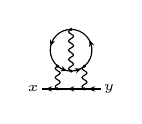
\begin{tikzpicture}[x=0.340cm, y=0.340cm, line width=0.420pt, baseline={([yshift=-0.6ex]0,0)}]
  \draw (0.500,0.000) -- (-0.500,0.000);
  \fill (-0.119,0.000) -- (0.119,-0.102) -- (0.042,0.000) -- (0.119,0.102) -- cycle;
  \draw (0.000,2.224) arc[start angle=90.000, end angle=229.997, radius=0.778];
  \fill (-0.772,1.600) -- (-0.594,1.789) -- (-0.717,1.751) -- (-0.786,1.859) -- cycle;
  \draw (0.000,0.668) arc[start angle=270.000, end angle=310.003, radius=0.778];
  \fill (0.378,0.756) -- (0.119,0.770) -- (0.227,0.701) -- (0.189,0.578) -- cycle;
  \draw (-0.500,0.850) arc[start angle=229.997, end angle=270.000, radius=0.778];
  \fill (-0.154,0.674) -- (-0.343,0.852) -- (-0.305,0.729) -- (-0.413,0.660) -- cycle;
  \draw (0.500,0.850) arc[start angle=310.003, end angle=450.000, radius=0.778];
  \fill (0.690,1.824) -- (0.676,1.565) -- (0.745,1.673) -- (0.868,1.635) -- cycle;
  \draw plot[smooth, tension=0.7] coordinates {(-0.500,0.000) (-0.565,0.042) (-0.592,0.085) (-0.565,0.128) (-0.500,0.170) (-0.435,0.213) (-0.408,0.255) (-0.435,0.298) (-0.500,0.340) (-0.565,0.383) (-0.592,0.425) (-0.565,0.468) (-0.500,0.510) (-0.435,0.553) (-0.408,0.595) (-0.435,0.638) (-0.500,0.680) (-0.565,0.723) (-0.592,0.765) (-0.565,0.808) (-0.500,0.850)};
  \draw plot[smooth, tension=0.7] coordinates {(0.500,0.000) (0.435,0.043) (0.408,0.085) (0.435,0.128) (0.500,0.170) (0.565,0.213) (0.592,0.255) (0.565,0.298) (0.500,0.340) (0.435,0.383) (0.408,0.425) (0.435,0.468) (0.500,0.510) (0.565,0.553) (0.592,0.595) (0.565,0.638) (0.500,0.680) (0.435,0.723) (0.408,0.765) (0.435,0.808) (0.500,0.850)};
  \draw plot[smooth, tension=0.7] coordinates {(0.000,0.668) (-0.066,0.711) (-0.093,0.754) (-0.066,0.798) (0.000,0.841) (0.066,0.884) (0.093,0.927) (0.066,0.970) (0.000,1.014) (-0.066,1.057) (-0.093,1.100) (-0.066,1.143) (0.000,1.187) (0.066,1.230) (0.093,1.273) (0.066,1.316) (0.000,1.359) (-0.066,1.403) (-0.093,1.446) (-0.066,1.489) (0.000,1.532) (0.066,1.575) (0.093,1.619) (0.066,1.662) (0.000,1.705) (-0.066,1.748) (-0.093,1.792) (-0.066,1.835) (0.000,1.878) (0.066,1.921) (0.093,1.964) (0.066,2.008) (0.000,2.051) (-0.066,2.094) (-0.093,2.137) (-0.066,2.180) (0.000,2.224)};
  \draw (-0.500,0.000) -- (-1.100,0.000);
  \fill (-0.949,0.000) -- (-0.711,-0.102) -- (-0.788,0.000) -- (-0.711,0.102) -- cycle;
  \draw (0.500,0.000) -- (1.100,0.000);
  \fill (0.651,0.000) -- (0.889,-0.102) -- (0.812,0.000) -- (0.889,0.102) -- cycle;
  \fill (-0.500,0.000) circle (0.064);
  \fill (0.500,0.000) circle (0.064);
  \fill (-0.500,0.850) circle (0.064);
  \fill (0.500,0.850) circle (0.064);
  \fill (0.000,0.668) circle (0.064);
  \fill (0.000,2.224) circle (0.064);
  \node[font=\tiny, inner sep=0pt, anchor=0] at (-1.190,0.000) {$x$};
  \node[font=\tiny, inner sep=0pt, anchor=180] at (1.190,0.000) {$y$};
\end{tikzpicture}}
\diagramgap
\mbox{$\displaystyle +\,$\,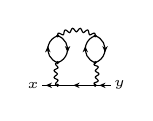
\begin{tikzpicture}[x=0.340cm, y=0.340cm, line width=0.420pt, baseline={([yshift=-0.6ex]0,0)}]
  \draw (0.700,0.000) -- (-0.700,0.000);
  \fill (-0.119,0.000) -- (0.119,-0.102) -- (0.042,0.000) -- (0.119,0.102) -- cycle;
  \draw (-0.700,1.850) arc[start angle=72.811, end angle=-72.811, radius=0.523];
  \fill (-0.331,1.231) -- (-0.229,1.469) -- (-0.331,1.392) -- (-0.433,1.469) -- cycle;
  \draw (-0.700,0.850) arc[start angle=252.811, end angle=107.189, radius=0.523];
  \fill (-1.069,1.469) -- (-1.171,1.231) -- (-1.069,1.308) -- (-0.967,1.231) -- cycle;
  \draw (0.700,1.850) arc[start angle=72.811, end angle=-72.811, radius=0.523];
  \fill (1.069,1.231) -- (1.171,1.469) -- (1.069,1.392) -- (0.967,1.469) -- cycle;
  \draw (0.700,0.850) arc[start angle=252.811, end angle=107.189, radius=0.523];
  \fill (0.331,1.469) -- (0.229,1.231) -- (0.331,1.308) -- (0.433,1.231) -- cycle;
  \draw plot[smooth, tension=0.7] coordinates {(-0.700,0.000) (-0.753,0.015) (-0.781,0.040) (-0.773,0.076) (-0.737,0.118) (-0.700,0.159) (-0.688,0.192) (-0.712,0.217) (-0.762,0.240) (-0.811,0.265) (-0.834,0.295) (-0.818,0.329) (-0.774,0.363) (-0.730,0.395) (-0.711,0.425) (-0.730,0.455) (-0.774,0.487) (-0.818,0.521) (-0.834,0.555) (-0.811,0.585) (-0.762,0.610) (-0.712,0.633) (-0.688,0.658) (-0.700,0.691) (-0.737,0.732) (-0.773,0.774) (-0.781,0.810) (-0.753,0.835) (-0.700,0.850)};
  \draw plot[smooth, tension=0.7] coordinates {(0.700,0.000) (0.667,0.044) (0.658,0.078) (0.685,0.101) (0.737,0.118) (0.789,0.138) (0.814,0.166) (0.801,0.201) (0.762,0.240) (0.721,0.276) (0.705,0.308) (0.727,0.336) (0.774,0.363) (0.821,0.393) (0.840,0.425) (0.821,0.457) (0.774,0.487) (0.727,0.514) (0.705,0.542) (0.721,0.574) (0.762,0.610) (0.801,0.649) (0.814,0.684) (0.789,0.712) (0.737,0.732) (0.685,0.749) (0.658,0.772) (0.667,0.806) (0.700,0.850)};
  \draw plot[smooth, tension=0.7] coordinates {(-0.700,1.850) (-0.699,1.911) (-0.680,1.947) (-0.639,1.947) (-0.585,1.921) (-0.532,1.892) (-0.494,1.887) (-0.473,1.920) (-0.462,1.978) (-0.448,2.037) (-0.422,2.068) (-0.381,2.060) (-0.334,2.022) (-0.289,1.983) (-0.253,1.970) (-0.226,1.997) (-0.202,2.052) (-0.175,2.106) (-0.143,2.131) (-0.106,2.114) (-0.068,2.066) (-0.032,2.018) (0.000,1.998) (0.032,2.018) (0.068,2.066) (0.106,2.114) (0.143,2.131) (0.175,2.106) (0.202,2.052) (0.226,1.997) (0.253,1.970) (0.289,1.983) (0.334,2.022) (0.381,2.060) (0.422,2.068) (0.448,2.037) (0.462,1.978) (0.473,1.920) (0.494,1.887) (0.532,1.892) (0.585,1.921) (0.639,1.947) (0.680,1.947) (0.699,1.911) (0.700,1.850)};
  \draw (-0.700,0.000) -- (-1.300,0.000);
  \fill (-1.149,0.000) -- (-0.911,-0.102) -- (-0.988,0.000) -- (-0.911,0.102) -- cycle;
  \draw (0.700,0.000) -- (1.300,0.000);
  \fill (0.851,0.000) -- (1.089,-0.102) -- (1.012,0.000) -- (1.089,0.102) -- cycle;
  \fill (-0.700,0.000) circle (0.064);
  \fill (0.700,0.000) circle (0.064);
  \fill (-0.700,0.850) circle (0.064);
  \fill (0.700,0.850) circle (0.064);
  \fill (-0.700,1.850) circle (0.064);
  \fill (0.700,1.850) circle (0.064);
  \node[font=\tiny, inner sep=0pt, anchor=0] at (-1.390,0.000) {$x$};
  \node[font=\tiny, inner sep=0pt, anchor=180] at (1.390,0.000) {$y$};
\end{tikzpicture}}
\diagramgap
\mbox{$\displaystyle +\,$\,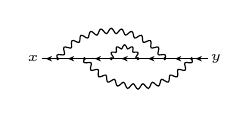
\begin{tikzpicture}[x=0.340cm, y=0.340cm, line width=0.420pt, baseline={([yshift=-0.6ex]0,0)}]
  \draw (-1.500,0.000) -- (-2.500,0.000);
  \fill (-2.119,0.000) -- (-1.881,-0.102) -- (-1.958,0.000) -- (-1.881,0.102) -- cycle;
  \draw (2.500,0.000) -- (1.500,0.000);
  \fill (1.881,0.000) -- (2.119,-0.102) -- (2.042,0.000) -- (2.119,0.102) -- cycle;
  \draw (-0.500,0.000) -- (-1.500,0.000);
  \fill (-1.119,0.000) -- (-0.881,-0.102) -- (-0.958,0.000) -- (-0.881,0.102) -- cycle;
  \draw (1.500,0.000) -- (0.500,0.000);
  \fill (0.881,0.000) -- (1.119,-0.102) -- (1.042,0.000) -- (1.119,0.102) -- cycle;
  \draw (0.500,0.000) -- (-0.500,0.000);
  \fill (-0.119,0.000) -- (0.119,-0.102) -- (0.042,0.000) -- (0.119,0.102) -- cycle;
  \draw plot[smooth, tension=0.7] coordinates {(0.500,0.000) (0.447,0.025) (0.421,0.050) (0.433,0.083) (0.468,0.130) (0.500,0.181) (0.501,0.224) (0.464,0.246) (0.404,0.247) (0.345,0.241) (0.311,0.249) (0.303,0.284) (0.311,0.342) (0.312,0.403) (0.291,0.440) (0.248,0.440) (0.196,0.410) (0.148,0.376) (0.114,0.365) (0.090,0.392) (0.067,0.446) (0.037,0.498) (0.000,0.520) (-0.037,0.498) (-0.067,0.446) (-0.090,0.392) (-0.114,0.365) (-0.148,0.376) (-0.196,0.410) (-0.248,0.440) (-0.291,0.440) (-0.312,0.403) (-0.311,0.342) (-0.303,0.284) (-0.311,0.249) (-0.345,0.241) (-0.404,0.247) (-0.464,0.246) (-0.501,0.224) (-0.500,0.181) (-0.468,0.130) (-0.433,0.083) (-0.421,0.050) (-0.447,0.025) (-0.500,0.000)};
  \draw plot[smooth, tension=0.7] coordinates {(-2.500,0.000) (-2.528,0.079) (-2.522,0.135) (-2.470,0.155) (-2.387,0.149) (-2.304,0.140) (-2.253,0.156) (-2.244,0.208) (-2.262,0.289) (-2.278,0.371) (-2.264,0.426) (-2.209,0.438) (-2.127,0.419) (-2.047,0.398) (-1.994,0.405) (-1.977,0.456) (-1.983,0.539) (-1.986,0.622) (-1.963,0.674) (-1.907,0.678) (-1.829,0.647) (-1.754,0.613) (-1.700,0.612) (-1.675,0.660) (-1.668,0.742) (-1.659,0.826) (-1.629,0.873) (-1.573,0.868) (-1.501,0.826) (-1.431,0.781) (-1.378,0.772) (-1.346,0.815) (-1.327,0.896) (-1.305,0.977) (-1.267,1.019) (-1.213,1.006) (-1.148,0.952) (-1.086,0.898) (-1.035,0.881) (-0.997,0.918) (-0.966,0.995) (-0.931,1.072) (-0.888,1.108) (-0.836,1.086) (-0.781,1.024) (-0.727,0.960) (-0.680,0.936) (-0.637,0.967) (-0.594,1.038) (-0.548,1.108) (-0.500,1.137) (-0.452,1.108) (-0.406,1.038) (-0.363,0.967) (-0.320,0.936) (-0.273,0.960) (-0.219,1.024) (-0.164,1.086) (-0.112,1.108) (-0.069,1.072) (-0.034,0.995) (-0.003,0.918) (0.035,0.881) (0.086,0.898) (0.148,0.952) (0.213,1.006) (0.267,1.019) (0.305,0.977) (0.327,0.896) (0.346,0.815) (0.378,0.772) (0.431,0.781) (0.501,0.826) (0.573,0.868) (0.629,0.873) (0.659,0.826) (0.668,0.742) (0.675,0.660) (0.700,0.612) (0.754,0.613) (0.829,0.647) (0.907,0.678) (0.963,0.674) (0.986,0.622) (0.983,0.539) (0.977,0.456) (0.994,0.405) (1.047,0.398) (1.127,0.419) (1.209,0.438) (1.264,0.426) (1.278,0.371) (1.262,0.289) (1.244,0.208) (1.253,0.156) (1.304,0.140) (1.387,0.149) (1.470,0.155) (1.522,0.135) (1.528,0.079) (1.500,0.000)};
  \draw plot[smooth, tension=0.7] coordinates {(2.500,0.000) (2.528,-0.079) (2.522,-0.135) (2.470,-0.155) (2.387,-0.149) (2.304,-0.140) (2.253,-0.156) (2.244,-0.208) (2.262,-0.289) (2.278,-0.371) (2.264,-0.426) (2.209,-0.438) (2.127,-0.419) (2.047,-0.398) (1.994,-0.405) (1.977,-0.456) (1.983,-0.539) (1.986,-0.622) (1.963,-0.674) (1.907,-0.678) (1.829,-0.647) (1.754,-0.613) (1.700,-0.612) (1.675,-0.660) (1.668,-0.742) (1.659,-0.826) (1.629,-0.873) (1.573,-0.868) (1.501,-0.826) (1.431,-0.781) (1.378,-0.772) (1.346,-0.815) (1.327,-0.896) (1.305,-0.977) (1.267,-1.019) (1.213,-1.006) (1.148,-0.952) (1.086,-0.898) (1.035,-0.881) (0.997,-0.918) (0.966,-0.995) (0.931,-1.072) (0.888,-1.108) (0.836,-1.086) (0.781,-1.024) (0.727,-0.960) (0.680,-0.936) (0.637,-0.967) (0.594,-1.038) (0.548,-1.108) (0.500,-1.137) (0.452,-1.108) (0.406,-1.038) (0.363,-0.967) (0.320,-0.936) (0.273,-0.960) (0.219,-1.024) (0.164,-1.086) (0.112,-1.108) (0.069,-1.072) (0.034,-0.995) (0.003,-0.918) (-0.035,-0.881) (-0.086,-0.898) (-0.148,-0.952) (-0.213,-1.006) (-0.267,-1.019) (-0.305,-0.977) (-0.327,-0.896) (-0.346,-0.815) (-0.378,-0.772) (-0.431,-0.781) (-0.501,-0.826) (-0.573,-0.868) (-0.629,-0.873) (-0.659,-0.826) (-0.668,-0.742) (-0.675,-0.660) (-0.700,-0.612) (-0.754,-0.613) (-0.829,-0.647) (-0.907,-0.678) (-0.963,-0.674) (-0.986,-0.622) (-0.983,-0.539) (-0.977,-0.456) (-0.994,-0.405) (-1.047,-0.398) (-1.127,-0.419) (-1.209,-0.438) (-1.264,-0.426) (-1.278,-0.371) (-1.262,-0.289) (-1.244,-0.208) (-1.253,-0.156) (-1.304,-0.140) (-1.387,-0.149) (-1.470,-0.155) (-1.522,-0.135) (-1.528,-0.079) (-1.500,0.000)};
  \draw (-2.500,0.000) -- (-3.100,0.000);
  \fill (-2.949,0.000) -- (-2.711,-0.102) -- (-2.788,0.000) -- (-2.711,0.102) -- cycle;
  \draw (2.500,0.000) -- (3.100,0.000);
  \fill (2.651,0.000) -- (2.889,-0.102) -- (2.812,0.000) -- (2.889,0.102) -- cycle;
  \fill (-2.500,0.000) circle (0.064);
  \fill (2.500,0.000) circle (0.064);
  \fill (1.500,0.000) circle (0.064);
  \fill (-1.500,0.000) circle (0.064);
  \fill (0.500,0.000) circle (0.064);
  \fill (-0.500,0.000) circle (0.064);
  \node[font=\tiny, inner sep=0pt, anchor=0] at (-3.190,0.000) {$x$};
  \node[font=\tiny, inner sep=0pt, anchor=180] at (3.190,0.000) {$y$};
\end{tikzpicture}}
\diagramgap
\mbox{$\displaystyle -\,$\,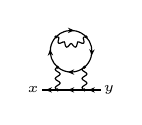
\begin{tikzpicture}[x=0.340cm, y=0.340cm, line width=0.420pt, baseline={([yshift=-0.6ex]0,0)}]
  \draw (0.500,0.000) -- (-0.500,0.000);
  \fill (-0.119,0.000) -- (0.119,-0.102) -- (0.042,0.000) -- (0.119,0.102) -- cycle;
  \draw (0.500,0.850) arc[start angle=310.003, end angle=229.997, radius=0.778];
  \fill (-0.119,0.668) -- (0.119,0.566) -- (0.042,0.668) -- (0.119,0.770) -- cycle;
  \draw (0.566,1.980) arc[start angle=43.334, end angle=-49.997, radius=0.778];
  \fill (0.770,1.281) -- (0.885,1.514) -- (0.779,1.442) -- (0.682,1.526) -- cycle;
  \draw (-0.500,0.850) arc[start angle=229.997, end angle=136.666, radius=0.778];
  \fill (-0.783,1.520) -- (-0.871,1.275) -- (-0.774,1.359) -- (-0.668,1.287) -- cycle;
  \draw (-0.566,1.980) arc[start angle=136.666, end angle=43.334, radius=0.778];
  \fill (0.119,2.224) -- (-0.119,2.326) -- (-0.042,2.224) -- (-0.119,2.122) -- cycle;
  \draw plot[smooth, tension=0.7] coordinates {(-0.566,1.980) (-0.499,1.979) (-0.461,1.965) (-0.457,1.924) (-0.474,1.860) (-0.485,1.792) (-0.469,1.748) (-0.422,1.740) (-0.358,1.764) (-0.298,1.792) (-0.257,1.797) (-0.236,1.762) (-0.222,1.697) (-0.202,1.632) (-0.168,1.599) (-0.122,1.613) (-0.075,1.662) (-0.035,1.715) (0.000,1.737) (0.035,1.715) (0.075,1.662) (0.122,1.613) (0.168,1.599) (0.202,1.632) (0.222,1.697) (0.236,1.762) (0.257,1.797) (0.298,1.792) (0.358,1.764) (0.422,1.740) (0.469,1.748) (0.485,1.792) (0.474,1.860) (0.457,1.924) (0.461,1.965) (0.499,1.979) (0.566,1.980)};
  \draw plot[smooth, tension=0.7] coordinates {(-0.500,0.000) (-0.565,0.042) (-0.592,0.085) (-0.565,0.128) (-0.500,0.170) (-0.435,0.213) (-0.408,0.255) (-0.435,0.298) (-0.500,0.340) (-0.565,0.383) (-0.592,0.425) (-0.565,0.468) (-0.500,0.510) (-0.435,0.553) (-0.408,0.595) (-0.435,0.638) (-0.500,0.680) (-0.565,0.723) (-0.592,0.765) (-0.565,0.808) (-0.500,0.850)};
  \draw plot[smooth, tension=0.7] coordinates {(0.500,0.000) (0.435,0.043) (0.408,0.085) (0.435,0.128) (0.500,0.170) (0.565,0.213) (0.592,0.255) (0.565,0.298) (0.500,0.340) (0.435,0.383) (0.408,0.425) (0.435,0.468) (0.500,0.510) (0.565,0.553) (0.592,0.595) (0.565,0.638) (0.500,0.680) (0.435,0.723) (0.408,0.765) (0.435,0.808) (0.500,0.850)};
  \draw (-0.500,0.000) -- (-1.100,0.000);
  \fill (-0.949,0.000) -- (-0.711,-0.102) -- (-0.788,0.000) -- (-0.711,0.102) -- cycle;
  \draw (0.500,0.000) -- (1.100,0.000);
  \fill (0.651,0.000) -- (0.889,-0.102) -- (0.812,0.000) -- (0.889,0.102) -- cycle;
  \fill (-0.500,0.000) circle (0.064);
  \fill (0.500,0.000) circle (0.064);
  \fill (-0.500,0.850) circle (0.064);
  \fill (0.500,0.850) circle (0.064);
  \fill (-0.566,1.980) circle (0.064);
  \fill (0.566,1.980) circle (0.064);
  \node[font=\tiny, inner sep=0pt, anchor=0] at (-1.190,0.000) {$x$};
  \node[font=\tiny, inner sep=0pt, anchor=180] at (1.190,0.000) {$y$};
\end{tikzpicture}}
\diagramgap
\mbox{$\displaystyle -\,$\,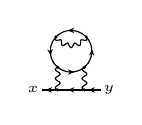
\begin{tikzpicture}[x=0.340cm, y=0.340cm, line width=0.420pt, baseline={([yshift=-0.6ex]0,0)}]
  \draw (0.500,0.000) -- (-0.500,0.000);
  \fill (-0.119,0.000) -- (0.119,-0.102) -- (0.042,0.000) -- (0.119,0.102) -- cycle;
  \draw (-0.566,1.980) arc[start angle=136.666, end angle=229.997, radius=0.778];
  \fill (-0.770,1.281) -- (-0.682,1.526) -- (-0.779,1.442) -- (-0.885,1.514) -- cycle;
  \draw (-0.500,0.850) arc[start angle=229.997, end angle=310.003, radius=0.778];
  \fill (0.119,0.668) -- (-0.119,0.770) -- (-0.042,0.668) -- (-0.119,0.566) -- cycle;
  \draw (0.500,0.850) arc[start angle=310.003, end angle=403.334, radius=0.778];
  \fill (0.783,1.520) -- (0.668,1.287) -- (0.774,1.359) -- (0.871,1.275) -- cycle;
  \draw (0.566,1.980) arc[start angle=43.334, end angle=136.666, radius=0.778];
  \fill (-0.119,2.224) -- (0.119,2.122) -- (0.042,2.224) -- (0.119,2.326) -- cycle;
  \draw plot[smooth, tension=0.7] coordinates {(0.566,1.980) (0.592,1.917) (0.586,1.869) (0.542,1.851) (0.474,1.860) (0.409,1.874) (0.369,1.869) (0.356,1.830) (0.358,1.764) (0.353,1.696) (0.327,1.656) (0.279,1.659) (0.222,1.697) (0.171,1.738) (0.132,1.752) (0.103,1.722) (0.075,1.662) (0.041,1.603) (0.000,1.579) (-0.041,1.603) (-0.075,1.662) (-0.103,1.722) (-0.132,1.752) (-0.171,1.738) (-0.222,1.697) (-0.279,1.659) (-0.327,1.656) (-0.353,1.696) (-0.358,1.764) (-0.356,1.830) (-0.369,1.869) (-0.409,1.874) (-0.474,1.860) (-0.542,1.851) (-0.586,1.869) (-0.592,1.917) (-0.566,1.980)};
  \draw plot[smooth, tension=0.7] coordinates {(-0.500,0.000) (-0.565,0.042) (-0.592,0.085) (-0.565,0.128) (-0.500,0.170) (-0.435,0.213) (-0.408,0.255) (-0.435,0.298) (-0.500,0.340) (-0.565,0.383) (-0.592,0.425) (-0.565,0.468) (-0.500,0.510) (-0.435,0.553) (-0.408,0.595) (-0.435,0.638) (-0.500,0.680) (-0.565,0.723) (-0.592,0.765) (-0.565,0.808) (-0.500,0.850)};
  \draw plot[smooth, tension=0.7] coordinates {(0.500,0.000) (0.435,0.043) (0.408,0.085) (0.435,0.128) (0.500,0.170) (0.565,0.213) (0.592,0.255) (0.565,0.298) (0.500,0.340) (0.435,0.383) (0.408,0.425) (0.435,0.468) (0.500,0.510) (0.565,0.553) (0.592,0.595) (0.565,0.638) (0.500,0.680) (0.435,0.723) (0.408,0.765) (0.435,0.808) (0.500,0.850)};
  \draw (-0.500,0.000) -- (-1.100,0.000);
  \fill (-0.949,0.000) -- (-0.711,-0.102) -- (-0.788,0.000) -- (-0.711,0.102) -- cycle;
  \draw (0.500,0.000) -- (1.100,0.000);
  \fill (0.651,0.000) -- (0.889,-0.102) -- (0.812,0.000) -- (0.889,0.102) -- cycle;
  \fill (-0.500,0.000) circle (0.064);
  \fill (0.500,0.000) circle (0.064);
  \fill (-0.500,0.850) circle (0.064);
  \fill (0.500,0.850) circle (0.064);
  \fill (0.566,1.980) circle (0.064);
  \fill (-0.566,1.980) circle (0.064);
  \node[font=\tiny, inner sep=0pt, anchor=0] at (-1.190,0.000) {$x$};
  \node[font=\tiny, inner sep=0pt, anchor=180] at (1.190,0.000) {$y$};
\end{tikzpicture}}
\diagramgap
\mbox{$\displaystyle -\,$\,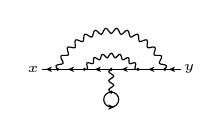
\begin{tikzpicture}[x=0.340cm, y=0.340cm, line width=0.420pt, baseline={([yshift=-0.6ex]0,0)}]
  \draw (-1.000,0.000) -- (-2.000,0.000);
  \fill (-1.619,0.000) -- (-1.381,-0.102) -- (-1.458,0.000) -- (-1.381,0.102) -- cycle;
  \draw (2.000,0.000) -- (1.000,0.000);
  \fill (1.381,0.000) -- (1.619,-0.102) -- (1.542,0.000) -- (1.619,0.102) -- cycle;
  \draw (0.000,0.000) -- (-1.000,0.000);
  \fill (-0.619,0.000) -- (-0.381,-0.102) -- (-0.458,0.000) -- (-0.381,0.102) -- cycle;
  \draw (1.000,0.000) -- (0.000,0.000);
  \fill (0.381,0.000) -- (0.619,-0.102) -- (0.542,0.000) -- (0.619,0.102) -- cycle;
  \draw plot[smooth, tension=0.7] coordinates {(-2.000,0.000) (-2.051,0.070) (-2.062,0.128) (-2.015,0.164) (-1.930,0.182) (-1.845,0.196) (-1.798,0.225) (-1.803,0.280) (-1.843,0.356) (-1.881,0.435) (-1.880,0.494) (-1.828,0.521) (-1.740,0.522) (-1.654,0.520) (-1.603,0.540) (-1.598,0.595) (-1.623,0.678) (-1.646,0.762) (-1.634,0.819) (-1.578,0.836) (-1.492,0.822) (-1.407,0.804) (-1.353,0.814) (-1.338,0.867) (-1.348,0.953) (-1.355,1.040) (-1.333,1.094) (-1.274,1.101) (-1.192,1.071) (-1.113,1.038) (-1.057,1.038) (-1.033,1.087) (-1.027,1.173) (-1.017,1.260) (-0.986,1.309) (-0.927,1.305) (-0.852,1.260) (-0.780,1.213) (-0.726,1.203) (-0.692,1.247) (-0.671,1.331) (-0.645,1.414) (-0.605,1.457) (-0.548,1.442) (-0.483,1.384) (-0.421,1.324) (-0.369,1.304) (-0.328,1.342) (-0.292,1.420) (-0.251,1.497) (-0.204,1.532) (-0.151,1.506) (-0.097,1.438) (-0.047,1.368) (0.000,1.339) (0.047,1.368) (0.097,1.438) (0.151,1.506) (0.204,1.532) (0.251,1.497) (0.292,1.420) (0.328,1.342) (0.369,1.304) (0.421,1.324) (0.483,1.384) (0.548,1.442) (0.605,1.457) (0.645,1.414) (0.671,1.331) (0.692,1.247) (0.726,1.203) (0.780,1.213) (0.852,1.260) (0.927,1.305) (0.986,1.309) (1.017,1.260) (1.027,1.173) (1.033,1.087) (1.057,1.038) (1.113,1.038) (1.192,1.071) (1.274,1.101) (1.333,1.094) (1.355,1.040) (1.348,0.953) (1.338,0.867) (1.353,0.814) (1.407,0.804) (1.492,0.822) (1.578,0.836) (1.634,0.819) (1.646,0.762) (1.623,0.678) (1.598,0.595) (1.603,0.540) (1.654,0.520) (1.740,0.522) (1.828,0.521) (1.880,0.494) (1.881,0.435) (1.843,0.356) (1.803,0.280) (1.798,0.225) (1.845,0.196) (1.930,0.182) (2.015,0.164) (2.062,0.128) (2.051,0.070) (2.000,0.000)};
  \draw plot[smooth, tension=0.7] coordinates {(0.000,-0.850) (-0.065,-0.808) (-0.092,-0.765) (-0.065,-0.722) (0.000,-0.680) (0.065,-0.638) (0.092,-0.595) (0.065,-0.552) (0.000,-0.510) (-0.065,-0.467) (-0.092,-0.425) (-0.065,-0.382) (0.000,-0.340) (0.065,-0.298) (0.092,-0.255) (0.065,-0.213) (0.000,-0.170) (-0.065,-0.127) (-0.092,-0.085) (-0.065,-0.042) (0.000,0.000)};
  \draw plot[smooth, tension=0.7] coordinates {(1.000,0.000) (0.931,-0.003) (0.890,0.012) (0.885,0.055) (0.902,0.122) (0.917,0.190) (0.904,0.236) (0.858,0.247) (0.790,0.230) (0.724,0.210) (0.680,0.214) (0.664,0.254) (0.665,0.323) (0.661,0.393) (0.638,0.434) (0.590,0.433) (0.529,0.400) (0.470,0.363) (0.427,0.356) (0.401,0.391) (0.384,0.458) (0.363,0.525) (0.330,0.559) (0.284,0.546) (0.233,0.498) (0.185,0.448) (0.145,0.429) (0.111,0.457) (0.078,0.518) (0.041,0.577) (0.000,0.601) (-0.041,0.577) (-0.078,0.518) (-0.111,0.457) (-0.145,0.429) (-0.185,0.448) (-0.233,0.498) (-0.284,0.546) (-0.330,0.559) (-0.363,0.525) (-0.384,0.458) (-0.401,0.391) (-0.427,0.356) (-0.470,0.363) (-0.529,0.400) (-0.590,0.433) (-0.638,0.434) (-0.661,0.393) (-0.665,0.323) (-0.664,0.254) (-0.680,0.214) (-0.724,0.210) (-0.790,0.230) (-0.858,0.247) (-0.904,0.236) (-0.917,0.190) (-0.902,0.122) (-0.885,0.055) (-0.890,0.012) (-0.931,-0.003) (-1.000,0.000)};
  \draw (0.000,-0.850) arc[start angle=90.000, end angle=450.000, radius=0.280];
  \fill (0.119,-1.410) -- (-0.119,-1.308) -- (-0.042,-1.410) -- (-0.119,-1.512) -- cycle;
  \draw (-2.000,0.000) -- (-2.600,0.000);
  \fill (-2.449,0.000) -- (-2.211,-0.102) -- (-2.288,0.000) -- (-2.211,0.102) -- cycle;
  \draw (2.000,0.000) -- (2.600,0.000);
  \fill (2.151,0.000) -- (2.389,-0.102) -- (2.312,0.000) -- (2.389,0.102) -- cycle;
  \fill (-2.000,0.000) circle (0.064);
  \fill (2.000,0.000) circle (0.064);
  \fill (0.000,-0.850) circle (0.064);
  \fill (1.000,0.000) circle (0.064);
  \fill (-1.000,0.000) circle (0.064);
  \fill (0.000,0.000) circle (0.064);
  \node[font=\tiny, inner sep=0pt, anchor=0] at (-2.690,0.000) {$x$};
  \node[font=\tiny, inner sep=0pt, anchor=180] at (2.690,0.000) {$y$};
\end{tikzpicture}}
\diagramgap
\mbox{$\displaystyle +\,$\,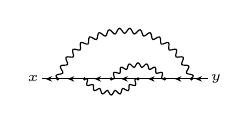
\begin{tikzpicture}[x=0.340cm, y=0.340cm, line width=0.420pt, baseline={([yshift=-0.6ex]0,0)}]
  \draw (-1.500,0.000) -- (-2.500,0.000);
  \fill (-2.119,0.000) -- (-1.881,-0.102) -- (-1.958,0.000) -- (-1.881,0.102) -- cycle;
  \draw (2.500,0.000) -- (1.500,0.000);
  \fill (1.881,0.000) -- (2.119,-0.102) -- (2.042,0.000) -- (2.119,0.102) -- cycle;
  \draw (-0.500,0.000) -- (-1.500,0.000);
  \fill (-1.119,0.000) -- (-0.881,-0.102) -- (-0.958,0.000) -- (-0.881,0.102) -- cycle;
  \draw (1.500,0.000) -- (0.500,0.000);
  \fill (0.881,0.000) -- (1.119,-0.102) -- (1.042,0.000) -- (1.119,0.102) -- cycle;
  \draw (0.500,0.000) -- (-0.500,0.000);
  \fill (-0.119,0.000) -- (0.119,-0.102) -- (0.042,0.000) -- (0.119,0.102) -- cycle;
  \draw plot[smooth, tension=0.7] coordinates {(-2.500,0.000) (-2.550,0.068) (-2.560,0.123) (-2.516,0.158) (-2.434,0.176) (-2.352,0.192) (-2.308,0.221) (-2.314,0.275) (-2.356,0.347) (-2.396,0.421) (-2.398,0.477) (-2.349,0.505) (-2.265,0.512) (-2.182,0.516) (-2.134,0.539) (-2.133,0.592) (-2.164,0.670) (-2.193,0.749) (-2.187,0.805) (-2.135,0.826) (-2.051,0.820) (-1.968,0.812) (-1.917,0.828) (-1.908,0.881) (-1.928,0.962) (-1.945,1.044) (-1.931,1.099) (-1.877,1.112) (-1.795,1.095) (-1.714,1.075) (-1.661,1.084) (-1.645,1.135) (-1.652,1.218) (-1.658,1.302) (-1.637,1.354) (-1.581,1.359) (-1.502,1.330) (-1.425,1.299) (-1.371,1.300) (-1.348,1.349) (-1.344,1.432) (-1.337,1.516) (-1.309,1.564) (-1.253,1.562) (-1.179,1.522) (-1.107,1.480) (-1.053,1.473) (-1.023,1.518) (-1.008,1.600) (-0.989,1.682) (-0.954,1.726) (-0.899,1.715) (-0.832,1.665) (-0.766,1.614) (-0.714,1.600) (-0.678,1.640) (-0.651,1.718) (-0.621,1.797) (-0.580,1.835) (-0.527,1.817) (-0.468,1.758) (-0.410,1.698) (-0.361,1.676) (-0.320,1.711) (-0.281,1.785) (-0.241,1.858) (-0.195,1.891) (-0.145,1.865) (-0.094,1.798) (-0.046,1.730) (0.000,1.702) (0.046,1.730) (0.094,1.798) (0.145,1.865) (0.195,1.891) (0.241,1.858) (0.281,1.785) (0.320,1.711) (0.361,1.676) (0.410,1.698) (0.468,1.758) (0.527,1.817) (0.580,1.835) (0.621,1.797) (0.651,1.718) (0.678,1.640) (0.714,1.600) (0.766,1.614) (0.832,1.665) (0.899,1.715) (0.954,1.726) (0.989,1.682) (1.008,1.600) (1.023,1.518) (1.053,1.473) (1.107,1.480) (1.179,1.522) (1.253,1.562) (1.309,1.564) (1.337,1.516) (1.344,1.432) (1.348,1.349) (1.371,1.300) (1.425,1.299) (1.502,1.330) (1.581,1.359) (1.637,1.354) (1.658,1.302) (1.652,1.218) (1.645,1.135) (1.661,1.084) (1.714,1.075) (1.795,1.095) (1.877,1.112) (1.931,1.099) (1.945,1.044) (1.928,0.962) (1.908,0.881) (1.917,0.828) (1.968,0.812) (2.051,0.820) (2.135,0.826) (2.187,0.805) (2.193,0.749) (2.164,0.670) (2.133,0.592) (2.134,0.539) (2.182,0.516) (2.265,0.512) (2.349,0.505) (2.398,0.477) (2.396,0.421) (2.356,0.347) (2.314,0.275) (2.308,0.221) (2.352,0.192) (2.434,0.176) (2.516,0.158) (2.560,0.123) (2.550,0.068) (2.500,0.000)};
  \draw plot[smooth, tension=0.7] coordinates {(1.500,0.000) (1.431,-0.003) (1.390,0.012) (1.385,0.055) (1.402,0.122) (1.417,0.190) (1.404,0.236) (1.358,0.247) (1.290,0.230) (1.224,0.210) (1.180,0.214) (1.164,0.254) (1.165,0.323) (1.161,0.393) (1.138,0.434) (1.090,0.433) (1.029,0.400) (0.970,0.363) (0.927,0.356) (0.901,0.391) (0.884,0.458) (0.863,0.525) (0.830,0.559) (0.784,0.546) (0.733,0.498) (0.685,0.448) (0.645,0.429) (0.611,0.457) (0.578,0.518) (0.541,0.577) (0.500,0.601) (0.459,0.577) (0.422,0.518) (0.389,0.457) (0.355,0.429) (0.315,0.448) (0.267,0.498) (0.216,0.546) (0.170,0.559) (0.137,0.525) (0.116,0.458) (0.099,0.391) (0.073,0.356) (0.030,0.363) (-0.029,0.400) (-0.090,0.433) (-0.138,0.434) (-0.161,0.393) (-0.165,0.323) (-0.164,0.254) (-0.180,0.214) (-0.224,0.210) (-0.290,0.230) (-0.358,0.247) (-0.404,0.236) (-0.417,0.190) (-0.402,0.122) (-0.385,0.055) (-0.390,0.012) (-0.431,-0.003) (-0.500,0.000)};
  \draw plot[smooth, tension=0.7] coordinates {(-1.500,0.000) (-1.431,0.003) (-1.390,-0.012) (-1.385,-0.055) (-1.402,-0.122) (-1.417,-0.190) (-1.404,-0.236) (-1.358,-0.247) (-1.290,-0.230) (-1.224,-0.210) (-1.180,-0.214) (-1.164,-0.254) (-1.165,-0.323) (-1.161,-0.393) (-1.138,-0.434) (-1.090,-0.433) (-1.029,-0.400) (-0.970,-0.363) (-0.927,-0.356) (-0.901,-0.391) (-0.884,-0.458) (-0.863,-0.525) (-0.830,-0.559) (-0.784,-0.546) (-0.733,-0.498) (-0.685,-0.448) (-0.645,-0.429) (-0.611,-0.457) (-0.578,-0.518) (-0.541,-0.577) (-0.500,-0.601) (-0.459,-0.577) (-0.422,-0.518) (-0.389,-0.457) (-0.355,-0.429) (-0.315,-0.448) (-0.267,-0.498) (-0.216,-0.546) (-0.170,-0.559) (-0.137,-0.525) (-0.116,-0.458) (-0.099,-0.391) (-0.073,-0.356) (-0.030,-0.363) (0.029,-0.400) (0.090,-0.433) (0.138,-0.434) (0.161,-0.393) (0.165,-0.323) (0.164,-0.254) (0.180,-0.214) (0.224,-0.210) (0.290,-0.230) (0.358,-0.247) (0.404,-0.236) (0.417,-0.190) (0.402,-0.122) (0.385,-0.055) (0.390,-0.012) (0.431,0.003) (0.500,0.000)};
  \draw (-2.500,0.000) -- (-3.100,0.000);
  \fill (-2.949,0.000) -- (-2.711,-0.102) -- (-2.788,0.000) -- (-2.711,0.102) -- cycle;
  \draw (2.500,0.000) -- (3.100,0.000);
  \fill (2.651,0.000) -- (2.889,-0.102) -- (2.812,0.000) -- (2.889,0.102) -- cycle;
  \fill (-2.500,0.000) circle (0.064);
  \fill (2.500,0.000) circle (0.064);
  \fill (1.500,0.000) circle (0.064);
  \fill (-1.500,0.000) circle (0.064);
  \fill (0.500,0.000) circle (0.064);
  \fill (-0.500,0.000) circle (0.064);
  \node[font=\tiny, inner sep=0pt, anchor=0] at (-3.190,0.000) {$x$};
  \node[font=\tiny, inner sep=0pt, anchor=180] at (3.190,0.000) {$y$};
\end{tikzpicture}}
\diagramgap
\mbox{$\displaystyle -\,$\,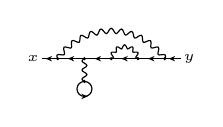
\begin{tikzpicture}[x=0.340cm, y=0.340cm, line width=0.420pt, baseline={([yshift=-0.6ex]0,0)}]
  \draw (-1.000,0.000) -- (-2.000,0.000);
  \fill (-1.619,0.000) -- (-1.381,-0.102) -- (-1.458,0.000) -- (-1.381,0.102) -- cycle;
  \draw (2.000,0.000) -- (1.000,0.000);
  \fill (1.381,0.000) -- (1.619,-0.102) -- (1.542,0.000) -- (1.619,0.102) -- cycle;
  \draw (0.000,0.000) -- (-1.000,0.000);
  \fill (-0.619,0.000) -- (-0.381,-0.102) -- (-0.458,0.000) -- (-0.381,0.102) -- cycle;
  \draw (1.000,0.000) -- (0.000,0.000);
  \fill (0.381,0.000) -- (0.619,-0.102) -- (0.542,0.000) -- (0.619,0.102) -- cycle;
  \draw plot[smooth, tension=0.7] coordinates {(1.000,0.000) (0.947,0.025) (0.921,0.050) (0.933,0.083) (0.968,0.130) (1.000,0.181) (1.001,0.224) (0.964,0.246) (0.904,0.247) (0.845,0.241) (0.811,0.249) (0.803,0.284) (0.811,0.342) (0.812,0.403) (0.791,0.440) (0.748,0.440) (0.696,0.410) (0.648,0.376) (0.614,0.365) (0.590,0.392) (0.567,0.446) (0.537,0.498) (0.500,0.520) (0.463,0.498) (0.433,0.446) (0.410,0.392) (0.386,0.365) (0.352,0.376) (0.304,0.410) (0.252,0.440) (0.209,0.440) (0.188,0.403) (0.189,0.342) (0.197,0.284) (0.189,0.249) (0.155,0.241) (0.096,0.247) (0.036,0.246) (-0.001,0.224) (0.000,0.181) (0.032,0.130) (0.067,0.083) (0.079,0.050) (0.053,0.025) (0.000,0.000)};
  \draw plot[smooth, tension=0.7] coordinates {(-2.000,0.000) (-2.028,0.079) (-2.022,0.135) (-1.970,0.155) (-1.887,0.149) (-1.804,0.140) (-1.753,0.156) (-1.744,0.208) (-1.762,0.289) (-1.778,0.371) (-1.764,0.426) (-1.709,0.438) (-1.627,0.419) (-1.547,0.398) (-1.494,0.405) (-1.477,0.456) (-1.483,0.539) (-1.486,0.622) (-1.463,0.674) (-1.407,0.678) (-1.329,0.647) (-1.254,0.613) (-1.200,0.612) (-1.175,0.660) (-1.168,0.742) (-1.159,0.826) (-1.129,0.873) (-1.073,0.868) (-1.001,0.826) (-0.931,0.781) (-0.878,0.772) (-0.846,0.815) (-0.827,0.896) (-0.805,0.977) (-0.767,1.019) (-0.713,1.006) (-0.648,0.952) (-0.586,0.898) (-0.535,0.881) (-0.497,0.918) (-0.466,0.995) (-0.431,1.072) (-0.388,1.108) (-0.336,1.086) (-0.281,1.024) (-0.227,0.960) (-0.180,0.936) (-0.137,0.967) (-0.094,1.038) (-0.048,1.108) (0.000,1.137) (0.048,1.108) (0.094,1.038) (0.137,0.967) (0.180,0.936) (0.227,0.960) (0.281,1.024) (0.336,1.086) (0.388,1.108) (0.431,1.072) (0.466,0.995) (0.497,0.918) (0.535,0.881) (0.586,0.898) (0.648,0.952) (0.713,1.006) (0.767,1.019) (0.805,0.977) (0.827,0.896) (0.846,0.815) (0.878,0.772) (0.931,0.781) (1.001,0.826) (1.073,0.868) (1.129,0.873) (1.159,0.826) (1.168,0.742) (1.175,0.660) (1.200,0.612) (1.254,0.613) (1.329,0.647) (1.407,0.678) (1.463,0.674) (1.486,0.622) (1.483,0.539) (1.477,0.456) (1.494,0.405) (1.547,0.398) (1.627,0.419) (1.709,0.438) (1.764,0.426) (1.778,0.371) (1.762,0.289) (1.744,0.208) (1.753,0.156) (1.804,0.140) (1.887,0.149) (1.970,0.155) (2.022,0.135) (2.028,0.079) (2.000,0.000)};
  \draw plot[smooth, tension=0.7] coordinates {(-1.000,-0.850) (-1.065,-0.808) (-1.092,-0.765) (-1.065,-0.722) (-1.000,-0.680) (-0.935,-0.638) (-0.908,-0.595) (-0.935,-0.552) (-1.000,-0.510) (-1.065,-0.467) (-1.092,-0.425) (-1.065,-0.382) (-1.000,-0.340) (-0.935,-0.298) (-0.908,-0.255) (-0.935,-0.213) (-1.000,-0.170) (-1.065,-0.127) (-1.092,-0.085) (-1.065,-0.042) (-1.000,0.000)};
  \draw (-1.000,-0.850) arc[start angle=90.000, end angle=450.000, radius=0.280];
  \fill (-0.881,-1.410) -- (-1.119,-1.308) -- (-1.042,-1.410) -- (-1.119,-1.512) -- cycle;
  \draw (-2.000,0.000) -- (-2.600,0.000);
  \fill (-2.449,0.000) -- (-2.211,-0.102) -- (-2.288,0.000) -- (-2.211,0.102) -- cycle;
  \draw (2.000,0.000) -- (2.600,0.000);
  \fill (2.151,0.000) -- (2.389,-0.102) -- (2.312,0.000) -- (2.389,0.102) -- cycle;
  \fill (-2.000,0.000) circle (0.064);
  \fill (2.000,0.000) circle (0.064);
  \fill (-1.000,-0.850) circle (0.064);
  \fill (1.000,0.000) circle (0.064);
  \fill (-1.000,0.000) circle (0.064);
  \fill (0.000,0.000) circle (0.064);
  \node[font=\tiny, inner sep=0pt, anchor=0] at (-2.690,0.000) {$x$};
  \node[font=\tiny, inner sep=0pt, anchor=180] at (2.690,0.000) {$y$};
\end{tikzpicture}}
\diagramgap
\mbox{$\displaystyle +\,$\,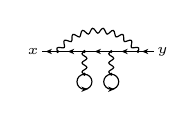
\begin{tikzpicture}[x=0.340cm, y=0.340cm, line width=0.420pt, baseline={([yshift=-0.6ex]0,0)}]
  \draw (-0.500,0.000) -- (-1.500,0.000);
  \fill (-1.119,0.000) -- (-0.881,-0.102) -- (-0.958,0.000) -- (-0.881,0.102) -- cycle;
  \draw (1.500,0.000) -- (0.500,0.000);
  \fill (0.881,0.000) -- (1.119,-0.102) -- (1.042,0.000) -- (1.119,0.102) -- cycle;
  \draw (0.500,0.000) -- (-0.500,0.000);
  \fill (-0.119,0.000) -- (0.119,-0.102) -- (0.042,0.000) -- (0.119,0.102) -- cycle;
  \draw plot[smooth, tension=0.7] coordinates {(-1.500,0.000) (-1.528,0.078) (-1.521,0.133) (-1.469,0.154) (-1.386,0.146) (-1.305,0.135) (-1.255,0.148) (-1.244,0.199) (-1.259,0.279) (-1.270,0.361) (-1.252,0.414) (-1.197,0.424) (-1.118,0.399) (-1.041,0.372) (-0.988,0.375) (-0.968,0.423) (-0.966,0.505) (-0.961,0.587) (-0.933,0.636) (-0.877,0.634) (-0.804,0.594) (-0.734,0.552) (-0.682,0.544) (-0.652,0.587) (-0.634,0.667) (-0.612,0.747) (-0.575,0.788) (-0.521,0.775) (-0.458,0.722) (-0.397,0.667) (-0.348,0.649) (-0.310,0.685) (-0.276,0.759) (-0.239,0.833) (-0.194,0.866) (-0.144,0.843) (-0.092,0.778) (-0.045,0.711) (0.000,0.684) (0.045,0.711) (0.092,0.778) (0.144,0.843) (0.194,0.866) (0.239,0.833) (0.276,0.759) (0.310,0.685) (0.348,0.649) (0.397,0.667) (0.458,0.722) (0.521,0.775) (0.575,0.788) (0.612,0.747) (0.634,0.667) (0.652,0.587) (0.682,0.544) (0.734,0.552) (0.804,0.594) (0.877,0.634) (0.933,0.636) (0.961,0.587) (0.966,0.505) (0.968,0.423) (0.988,0.375) (1.041,0.372) (1.118,0.399) (1.197,0.424) (1.252,0.414) (1.270,0.361) (1.259,0.279) (1.244,0.199) (1.255,0.148) (1.305,0.135) (1.386,0.146) (1.469,0.154) (1.521,0.133) (1.528,0.078) (1.500,0.000)};
  \draw plot[smooth, tension=0.7] coordinates {(0.500,-0.850) (0.435,-0.808) (0.408,-0.765) (0.435,-0.722) (0.500,-0.680) (0.565,-0.638) (0.592,-0.595) (0.565,-0.552) (0.500,-0.510) (0.435,-0.467) (0.408,-0.425) (0.435,-0.382) (0.500,-0.340) (0.565,-0.298) (0.592,-0.255) (0.565,-0.213) (0.500,-0.170) (0.435,-0.127) (0.408,-0.085) (0.435,-0.042) (0.500,0.000)};
  \draw plot[smooth, tension=0.7] coordinates {(-0.500,-0.850) (-0.565,-0.808) (-0.592,-0.765) (-0.565,-0.722) (-0.500,-0.680) (-0.435,-0.638) (-0.408,-0.595) (-0.435,-0.552) (-0.500,-0.510) (-0.565,-0.467) (-0.592,-0.425) (-0.565,-0.382) (-0.500,-0.340) (-0.435,-0.298) (-0.408,-0.255) (-0.435,-0.213) (-0.500,-0.170) (-0.565,-0.127) (-0.592,-0.085) (-0.565,-0.042) (-0.500,0.000)};
  \draw (0.500,-0.850) arc[start angle=90.000, end angle=450.000, radius=0.280];
  \fill (0.619,-1.410) -- (0.381,-1.308) -- (0.458,-1.410) -- (0.381,-1.512) -- cycle;
  \draw (-0.500,-0.850) arc[start angle=90.000, end angle=450.000, radius=0.280];
  \fill (-0.381,-1.410) -- (-0.619,-1.308) -- (-0.542,-1.410) -- (-0.619,-1.512) -- cycle;
  \draw (-1.500,0.000) -- (-2.100,0.000);
  \fill (-1.949,0.000) -- (-1.711,-0.102) -- (-1.788,0.000) -- (-1.711,0.102) -- cycle;
  \draw (1.500,0.000) -- (2.100,0.000);
  \fill (1.651,0.000) -- (1.889,-0.102) -- (1.812,0.000) -- (1.889,0.102) -- cycle;
  \fill (-1.500,0.000) circle (0.064);
  \fill (1.500,0.000) circle (0.064);
  \fill (0.500,-0.850) circle (0.064);
  \fill (-0.500,-0.850) circle (0.064);
  \fill (0.500,0.000) circle (0.064);
  \fill (-0.500,0.000) circle (0.064);
  \node[font=\tiny, inner sep=0pt, anchor=0] at (-2.190,0.000) {$x$};
  \node[font=\tiny, inner sep=0pt, anchor=180] at (2.190,0.000) {$y$};
\end{tikzpicture}}
\diagramgap
\mbox{$\displaystyle +\,$\,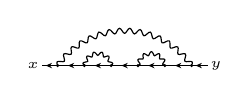
\begin{tikzpicture}[x=0.340cm, y=0.340cm, line width=0.420pt, baseline={([yshift=-0.6ex]0,0)}]
  \draw (-1.500,0.000) -- (-2.500,0.000);
  \fill (-2.119,0.000) -- (-1.881,-0.102) -- (-1.958,0.000) -- (-1.881,0.102) -- cycle;
  \draw (2.500,0.000) -- (1.500,0.000);
  \fill (1.881,0.000) -- (2.119,-0.102) -- (2.042,0.000) -- (2.119,0.102) -- cycle;
  \draw (-0.500,0.000) -- (-1.500,0.000);
  \fill (-1.119,0.000) -- (-0.881,-0.102) -- (-0.958,0.000) -- (-0.881,0.102) -- cycle;
  \draw plot[smooth, tension=0.7] coordinates {(-1.500,0.000) (-1.544,0.042) (-1.556,0.082) (-1.527,0.113) (-1.468,0.130) (-1.411,0.140) (-1.379,0.157) (-1.381,0.193) (-1.404,0.247) (-1.421,0.305) (-1.410,0.346) (-1.369,0.358) (-1.311,0.342) (-1.256,0.322) (-1.220,0.320) (-1.204,0.352) (-1.196,0.410) (-1.181,0.469) (-1.151,0.499) (-1.110,0.488) (-1.067,0.446) (-1.030,0.400) (-1.000,0.380) (-0.970,0.400) (-0.933,0.446) (-0.890,0.488) (-0.849,0.499) (-0.819,0.469) (-0.804,0.410) (-0.796,0.352) (-0.780,0.320) (-0.744,0.322) (-0.689,0.342) (-0.631,0.358) (-0.590,0.346) (-0.579,0.305) (-0.596,0.247) (-0.619,0.193) (-0.621,0.157) (-0.589,0.140) (-0.532,0.130) (-0.473,0.113) (-0.444,0.082) (-0.456,0.042) (-0.500,0.000)};
  \draw (1.500,0.000) -- (0.500,0.000);
  \fill (0.881,0.000) -- (1.119,-0.102) -- (1.042,0.000) -- (1.119,0.102) -- cycle;
  \draw plot[smooth, tension=0.7] coordinates {(1.500,0.000) (1.447,0.025) (1.421,0.050) (1.433,0.083) (1.468,0.130) (1.500,0.181) (1.501,0.224) (1.464,0.246) (1.404,0.247) (1.345,0.241) (1.311,0.249) (1.303,0.284) (1.311,0.342) (1.312,0.403) (1.291,0.440) (1.248,0.440) (1.196,0.410) (1.148,0.376) (1.114,0.365) (1.090,0.392) (1.067,0.446) (1.037,0.498) (1.000,0.520) (0.963,0.498) (0.933,0.446) (0.910,0.392) (0.886,0.365) (0.852,0.376) (0.804,0.410) (0.752,0.440) (0.709,0.440) (0.688,0.403) (0.689,0.342) (0.697,0.284) (0.689,0.249) (0.655,0.241) (0.596,0.247) (0.536,0.246) (0.499,0.224) (0.500,0.181) (0.532,0.130) (0.567,0.083) (0.579,0.050) (0.553,0.025) (0.500,0.000)};
  \draw (0.500,0.000) -- (-0.500,0.000);
  \fill (-0.119,0.000) -- (0.119,-0.102) -- (0.042,0.000) -- (0.119,0.102) -- cycle;
  \draw plot[smooth, tension=0.7] coordinates {(-2.500,0.000) (-2.529,0.079) (-2.523,0.135) (-2.471,0.157) (-2.387,0.151) (-2.303,0.144) (-2.252,0.161) (-2.244,0.214) (-2.264,0.295) (-2.283,0.377) (-2.271,0.432) (-2.216,0.447) (-2.133,0.431) (-2.052,0.414) (-1.998,0.424) (-1.984,0.476) (-1.994,0.559) (-2.003,0.643) (-1.984,0.696) (-1.928,0.704) (-1.847,0.678) (-1.768,0.650) (-1.714,0.654) (-1.693,0.704) (-1.693,0.787) (-1.692,0.872) (-1.666,0.922) (-1.610,0.923) (-1.533,0.887) (-1.458,0.850) (-1.404,0.847) (-1.377,0.894) (-1.367,0.977) (-1.355,1.060) (-1.323,1.107) (-1.267,1.101) (-1.195,1.056) (-1.126,1.010) (-1.072,1.000) (-1.039,1.044) (-1.019,1.125) (-0.997,1.206) (-0.960,1.249) (-0.905,1.236) (-0.839,1.182) (-0.776,1.128) (-0.724,1.112) (-0.686,1.151) (-0.656,1.229) (-0.624,1.307) (-0.582,1.344) (-0.529,1.324) (-0.470,1.264) (-0.414,1.202) (-0.365,1.179) (-0.323,1.213) (-0.283,1.287) (-0.241,1.360) (-0.195,1.392) (-0.145,1.366) (-0.094,1.299) (-0.046,1.230) (0.000,1.202) (0.046,1.230) (0.094,1.299) (0.145,1.366) (0.195,1.392) (0.241,1.360) (0.283,1.287) (0.323,1.213) (0.365,1.179) (0.414,1.202) (0.470,1.264) (0.529,1.324) (0.582,1.344) (0.624,1.307) (0.656,1.229) (0.686,1.151) (0.724,1.112) (0.776,1.128) (0.839,1.182) (0.905,1.236) (0.960,1.249) (0.997,1.206) (1.019,1.125) (1.039,1.044) (1.072,1.000) (1.126,1.010) (1.195,1.056) (1.267,1.101) (1.323,1.107) (1.355,1.060) (1.367,0.977) (1.377,0.894) (1.404,0.847) (1.458,0.850) (1.533,0.887) (1.610,0.923) (1.666,0.922) (1.692,0.872) (1.693,0.787) (1.693,0.704) (1.714,0.654) (1.768,0.650) (1.847,0.678) (1.928,0.704) (1.984,0.696) (2.003,0.643) (1.994,0.559) (1.984,0.476) (1.998,0.424) (2.052,0.414) (2.133,0.431) (2.216,0.447) (2.271,0.432) (2.283,0.377) (2.264,0.295) (2.244,0.214) (2.252,0.161) (2.303,0.144) (2.387,0.151) (2.471,0.157) (2.523,0.135) (2.529,0.079) (2.500,0.000)};
  \draw (-2.500,0.000) -- (-3.100,0.000);
  \fill (-2.949,0.000) -- (-2.711,-0.102) -- (-2.788,0.000) -- (-2.711,0.102) -- cycle;
  \draw (2.500,0.000) -- (3.100,0.000);
  \fill (2.651,0.000) -- (2.889,-0.102) -- (2.812,0.000) -- (2.889,0.102) -- cycle;
  \fill (-2.500,0.000) circle (0.064);
  \fill (2.500,0.000) circle (0.064);
  \fill (1.500,0.000) circle (0.064);
  \fill (-1.500,0.000) circle (0.064);
  \fill (0.500,0.000) circle (0.064);
  \fill (-0.500,0.000) circle (0.064);
  \node[font=\tiny, inner sep=0pt, anchor=0] at (-3.190,0.000) {$x$};
  \node[font=\tiny, inner sep=0pt, anchor=180] at (3.190,0.000) {$y$};
\end{tikzpicture}}
\diagramgap
\mbox{$\displaystyle +\,$\,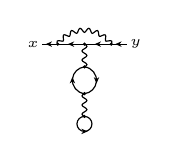
\begin{tikzpicture}[x=0.340cm, y=0.340cm, line width=0.420pt, baseline={([yshift=-0.6ex]0,0)}]
  \draw (0.000,0.000) -- (-1.000,0.000);
  \fill (-0.619,0.000) -- (-0.381,-0.102) -- (-0.458,0.000) -- (-0.381,0.102) -- cycle;
  \draw (1.000,0.000) -- (0.000,0.000);
  \fill (0.381,0.000) -- (0.619,-0.102) -- (0.542,0.000) -- (0.619,0.102) -- cycle;
  \draw (0.000,-0.850) arc[start angle=83.974, end angle=-83.974, radius=0.503];
  \fill (0.450,-1.469) -- (0.552,-1.231) -- (0.450,-1.308) -- (0.348,-1.231) -- cycle;
  \draw (0.000,-1.850) arc[start angle=263.974, end angle=96.026, radius=0.503];
  \fill (-0.450,-1.231) -- (-0.552,-1.469) -- (-0.450,-1.392) -- (-0.348,-1.469) -- cycle;
  \draw plot[smooth, tension=0.7] coordinates {(-1.000,0.000) (-1.023,0.066) (-1.017,0.113) (-0.972,0.130) (-0.902,0.122) (-0.834,0.110) (-0.792,0.119) (-0.781,0.162) (-0.790,0.230) (-0.796,0.300) (-0.777,0.344) (-0.730,0.349) (-0.665,0.323) (-0.602,0.295) (-0.558,0.293) (-0.537,0.331) (-0.529,0.400) (-0.516,0.469) (-0.488,0.507) (-0.441,0.499) (-0.384,0.458) (-0.330,0.415) (-0.288,0.402) (-0.258,0.434) (-0.233,0.498) (-0.204,0.561) (-0.166,0.591) (-0.122,0.572) (-0.078,0.518) (-0.037,0.462) (0.000,0.439) (0.037,0.462) (0.078,0.518) (0.122,0.572) (0.166,0.591) (0.204,0.561) (0.233,0.498) (0.258,0.434) (0.288,0.402) (0.330,0.415) (0.384,0.458) (0.441,0.499) (0.488,0.507) (0.516,0.469) (0.529,0.400) (0.537,0.331) (0.558,0.293) (0.602,0.295) (0.665,0.323) (0.730,0.349) (0.777,0.344) (0.796,0.300) (0.790,0.230) (0.781,0.162) (0.792,0.119) (0.834,0.110) (0.902,0.122) (0.972,0.130) (1.017,0.113) (1.023,0.066) (1.000,0.000)};
  \draw plot[smooth, tension=0.7] coordinates {(0.000,-2.700) (-0.065,-2.658) (-0.092,-2.615) (-0.065,-2.573) (0.000,-2.530) (0.065,-2.488) (0.092,-2.445) (0.065,-2.403) (0.000,-2.360) (-0.065,-2.318) (-0.092,-2.275) (-0.065,-2.232) (0.000,-2.190) (0.065,-2.148) (0.092,-2.105) (0.065,-2.062) (0.000,-2.020) (-0.065,-1.978) (-0.092,-1.935) (-0.065,-1.892) (0.000,-1.850)};
  \draw plot[smooth, tension=0.7] coordinates {(0.000,0.000) (0.065,-0.042) (0.092,-0.085) (0.065,-0.128) (0.000,-0.170) (-0.065,-0.212) (-0.092,-0.255) (-0.065,-0.298) (0.000,-0.340) (0.065,-0.382) (0.092,-0.425) (0.065,-0.468) (0.000,-0.510) (-0.065,-0.552) (-0.092,-0.595) (-0.065,-0.638) (0.000,-0.680) (0.065,-0.722) (0.092,-0.765) (0.065,-0.808) (0.000,-0.850)};
  \draw (0.000,-2.700) arc[start angle=90.000, end angle=450.000, radius=0.280];
  \fill (0.119,-3.260) -- (-0.119,-3.158) -- (-0.042,-3.260) -- (-0.119,-3.362) -- cycle;
  \draw (-1.000,0.000) -- (-1.600,0.000);
  \fill (-1.449,0.000) -- (-1.211,-0.102) -- (-1.288,0.000) -- (-1.211,0.102) -- cycle;
  \draw (1.000,0.000) -- (1.600,0.000);
  \fill (1.151,0.000) -- (1.389,-0.102) -- (1.312,0.000) -- (1.389,0.102) -- cycle;
  \fill (-1.000,0.000) circle (0.064);
  \fill (1.000,0.000) circle (0.064);
  \fill (0.000,-2.700) circle (0.064);
  \fill (0.000,0.000) circle (0.064);
  \fill (0.000,-1.850) circle (0.064);
  \fill (0.000,-0.850) circle (0.064);
  \node[font=\tiny, inner sep=0pt, anchor=0] at (-1.690,0.000) {$x$};
  \node[font=\tiny, inner sep=0pt, anchor=180] at (1.690,0.000) {$y$};
\end{tikzpicture}}
\diagramgap
\mbox{$\displaystyle -\,$\,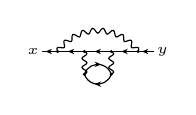
\begin{tikzpicture}[x=0.340cm, y=0.340cm, line width=0.420pt, baseline={([yshift=-0.6ex]0,0)}]
  \draw (-0.500,0.000) -- (-1.500,0.000);
  \fill (-1.119,0.000) -- (-0.881,-0.102) -- (-0.958,0.000) -- (-0.881,0.102) -- cycle;
  \draw (1.500,0.000) -- (0.500,0.000);
  \fill (0.881,0.000) -- (1.119,-0.102) -- (1.042,0.000) -- (1.119,0.102) -- cycle;
  \draw (0.500,0.000) -- (-0.500,0.000);
  \fill (-0.119,0.000) -- (0.119,-0.102) -- (0.042,0.000) -- (0.119,0.102) -- cycle;
  \draw (-0.500,-0.850) arc[start angle=162.811, end angle=17.189, radius=0.523];
  \fill (0.119,-0.481) -- (-0.119,-0.379) -- (-0.042,-0.481) -- (-0.119,-0.583) -- cycle;
  \draw (0.500,-0.850) arc[start angle=342.811, end angle=197.189, radius=0.523];
  \fill (-0.119,-1.219) -- (0.119,-1.321) -- (0.042,-1.219) -- (0.119,-1.117) -- cycle;
  \draw plot[smooth, tension=0.7] coordinates {(-1.500,0.000) (-1.528,0.078) (-1.521,0.133) (-1.469,0.154) (-1.386,0.146) (-1.305,0.135) (-1.255,0.148) (-1.244,0.199) (-1.259,0.279) (-1.270,0.361) (-1.252,0.414) (-1.197,0.424) (-1.118,0.399) (-1.041,0.372) (-0.988,0.375) (-0.968,0.423) (-0.966,0.505) (-0.961,0.587) (-0.933,0.636) (-0.877,0.634) (-0.804,0.594) (-0.734,0.552) (-0.682,0.544) (-0.652,0.587) (-0.634,0.667) (-0.612,0.747) (-0.575,0.788) (-0.521,0.775) (-0.458,0.722) (-0.397,0.667) (-0.348,0.649) (-0.310,0.685) (-0.276,0.759) (-0.239,0.833) (-0.194,0.866) (-0.144,0.843) (-0.092,0.778) (-0.045,0.711) (0.000,0.684) (0.045,0.711) (0.092,0.778) (0.144,0.843) (0.194,0.866) (0.239,0.833) (0.276,0.759) (0.310,0.685) (0.348,0.649) (0.397,0.667) (0.458,0.722) (0.521,0.775) (0.575,0.788) (0.612,0.747) (0.634,0.667) (0.652,0.587) (0.682,0.544) (0.734,0.552) (0.804,0.594) (0.877,0.634) (0.933,0.636) (0.961,0.587) (0.966,0.505) (0.968,0.423) (0.988,0.375) (1.041,0.372) (1.118,0.399) (1.197,0.424) (1.252,0.414) (1.270,0.361) (1.259,0.279) (1.244,0.199) (1.255,0.148) (1.305,0.135) (1.386,0.146) (1.469,0.154) (1.521,0.133) (1.528,0.078) (1.500,0.000)};
  \draw plot[smooth, tension=0.7] coordinates {(0.500,0.000) (0.565,-0.042) (0.592,-0.085) (0.565,-0.128) (0.500,-0.170) (0.435,-0.212) (0.408,-0.255) (0.435,-0.298) (0.500,-0.340) (0.565,-0.382) (0.592,-0.425) (0.565,-0.468) (0.500,-0.510) (0.435,-0.552) (0.408,-0.595) (0.435,-0.638) (0.500,-0.680) (0.565,-0.722) (0.592,-0.765) (0.565,-0.808) (0.500,-0.850)};
  \draw plot[smooth, tension=0.7] coordinates {(-0.500,0.000) (-0.435,-0.042) (-0.408,-0.085) (-0.435,-0.128) (-0.500,-0.170) (-0.565,-0.212) (-0.592,-0.255) (-0.565,-0.298) (-0.500,-0.340) (-0.435,-0.382) (-0.408,-0.425) (-0.435,-0.468) (-0.500,-0.510) (-0.565,-0.552) (-0.592,-0.595) (-0.565,-0.638) (-0.500,-0.680) (-0.435,-0.722) (-0.408,-0.765) (-0.435,-0.808) (-0.500,-0.850)};
  \draw (-1.500,0.000) -- (-2.100,0.000);
  \fill (-1.949,0.000) -- (-1.711,-0.102) -- (-1.788,0.000) -- (-1.711,0.102) -- cycle;
  \draw (1.500,0.000) -- (2.100,0.000);
  \fill (1.651,0.000) -- (1.889,-0.102) -- (1.812,0.000) -- (1.889,0.102) -- cycle;
  \fill (-1.500,0.000) circle (0.064);
  \fill (1.500,0.000) circle (0.064);
  \fill (0.500,0.000) circle (0.064);
  \fill (-0.500,0.000) circle (0.064);
  \fill (0.500,-0.850) circle (0.064);
  \fill (-0.500,-0.850) circle (0.064);
  \node[font=\tiny, inner sep=0pt, anchor=0] at (-2.190,0.000) {$x$};
  \node[font=\tiny, inner sep=0pt, anchor=180] at (2.190,0.000) {$y$};
\end{tikzpicture}}
\diagramgap
\mbox{$\displaystyle -\,$\,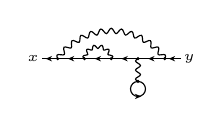
\begin{tikzpicture}[x=0.340cm, y=0.340cm, line width=0.420pt, baseline={([yshift=-0.6ex]0,0)}]
  \draw (-1.000,0.000) -- (-2.000,0.000);
  \fill (-1.619,0.000) -- (-1.381,-0.102) -- (-1.458,0.000) -- (-1.381,0.102) -- cycle;
  \draw (2.000,0.000) -- (1.000,0.000);
  \fill (1.381,0.000) -- (1.619,-0.102) -- (1.542,0.000) -- (1.619,0.102) -- cycle;
  \draw (0.000,0.000) -- (-1.000,0.000);
  \fill (-0.619,0.000) -- (-0.381,-0.102) -- (-0.458,0.000) -- (-0.381,0.102) -- cycle;
  \draw plot[smooth, tension=0.7] coordinates {(-1.000,0.000) (-1.044,0.042) (-1.056,0.082) (-1.027,0.113) (-0.968,0.130) (-0.911,0.140) (-0.879,0.157) (-0.881,0.193) (-0.904,0.247) (-0.921,0.305) (-0.910,0.346) (-0.869,0.358) (-0.811,0.342) (-0.756,0.322) (-0.720,0.320) (-0.704,0.352) (-0.696,0.410) (-0.681,0.469) (-0.651,0.499) (-0.610,0.488) (-0.567,0.446) (-0.530,0.400) (-0.500,0.380) (-0.470,0.400) (-0.433,0.446) (-0.390,0.488) (-0.349,0.499) (-0.319,0.469) (-0.304,0.410) (-0.296,0.352) (-0.280,0.320) (-0.244,0.322) (-0.189,0.342) (-0.131,0.358) (-0.090,0.346) (-0.079,0.305) (-0.096,0.247) (-0.119,0.193) (-0.121,0.157) (-0.089,0.140) (-0.032,0.130) (0.027,0.113) (0.056,0.082) (0.044,0.042) (0.000,0.000)};
  \draw (1.000,0.000) -- (0.000,0.000);
  \fill (0.381,0.000) -- (0.619,-0.102) -- (0.542,0.000) -- (0.619,0.102) -- cycle;
  \draw plot[smooth, tension=0.7] coordinates {(-2.000,0.000) (-2.028,0.079) (-2.022,0.135) (-1.970,0.155) (-1.887,0.149) (-1.804,0.140) (-1.753,0.156) (-1.744,0.208) (-1.762,0.289) (-1.778,0.371) (-1.764,0.426) (-1.709,0.438) (-1.627,0.419) (-1.547,0.398) (-1.494,0.405) (-1.477,0.456) (-1.483,0.539) (-1.486,0.622) (-1.463,0.674) (-1.407,0.678) (-1.329,0.647) (-1.254,0.613) (-1.200,0.612) (-1.175,0.660) (-1.168,0.742) (-1.159,0.826) (-1.129,0.873) (-1.073,0.868) (-1.001,0.826) (-0.931,0.781) (-0.878,0.772) (-0.846,0.815) (-0.827,0.896) (-0.805,0.977) (-0.767,1.019) (-0.713,1.006) (-0.648,0.952) (-0.586,0.898) (-0.535,0.881) (-0.497,0.918) (-0.466,0.995) (-0.431,1.072) (-0.388,1.108) (-0.336,1.086) (-0.281,1.024) (-0.227,0.960) (-0.180,0.936) (-0.137,0.967) (-0.094,1.038) (-0.048,1.108) (0.000,1.137) (0.048,1.108) (0.094,1.038) (0.137,0.967) (0.180,0.936) (0.227,0.960) (0.281,1.024) (0.336,1.086) (0.388,1.108) (0.431,1.072) (0.466,0.995) (0.497,0.918) (0.535,0.881) (0.586,0.898) (0.648,0.952) (0.713,1.006) (0.767,1.019) (0.805,0.977) (0.827,0.896) (0.846,0.815) (0.878,0.772) (0.931,0.781) (1.001,0.826) (1.073,0.868) (1.129,0.873) (1.159,0.826) (1.168,0.742) (1.175,0.660) (1.200,0.612) (1.254,0.613) (1.329,0.647) (1.407,0.678) (1.463,0.674) (1.486,0.622) (1.483,0.539) (1.477,0.456) (1.494,0.405) (1.547,0.398) (1.627,0.419) (1.709,0.438) (1.764,0.426) (1.778,0.371) (1.762,0.289) (1.744,0.208) (1.753,0.156) (1.804,0.140) (1.887,0.149) (1.970,0.155) (2.022,0.135) (2.028,0.079) (2.000,0.000)};
  \draw plot[smooth, tension=0.7] coordinates {(1.000,-0.850) (0.935,-0.808) (0.908,-0.765) (0.935,-0.722) (1.000,-0.680) (1.065,-0.638) (1.092,-0.595) (1.065,-0.552) (1.000,-0.510) (0.935,-0.467) (0.908,-0.425) (0.935,-0.382) (1.000,-0.340) (1.065,-0.298) (1.092,-0.255) (1.065,-0.213) (1.000,-0.170) (0.935,-0.127) (0.908,-0.085) (0.935,-0.042) (1.000,0.000)};
  \draw (1.000,-0.850) arc[start angle=90.000, end angle=450.000, radius=0.280];
  \fill (1.119,-1.410) -- (0.881,-1.308) -- (0.958,-1.410) -- (0.881,-1.512) -- cycle;
  \draw (-2.000,0.000) -- (-2.600,0.000);
  \fill (-2.449,0.000) -- (-2.211,-0.102) -- (-2.288,0.000) -- (-2.211,0.102) -- cycle;
  \draw (2.000,0.000) -- (2.600,0.000);
  \fill (2.151,0.000) -- (2.389,-0.102) -- (2.312,0.000) -- (2.389,0.102) -- cycle;
  \fill (-2.000,0.000) circle (0.064);
  \fill (2.000,0.000) circle (0.064);
  \fill (1.000,-0.850) circle (0.064);
  \fill (1.000,0.000) circle (0.064);
  \fill (-1.000,0.000) circle (0.064);
  \fill (0.000,0.000) circle (0.064);
  \node[font=\tiny, inner sep=0pt, anchor=0] at (-2.690,0.000) {$x$};
  \node[font=\tiny, inner sep=0pt, anchor=180] at (2.690,0.000) {$y$};
\end{tikzpicture}}
\diagramgap
\mbox{$\displaystyle +\,$\,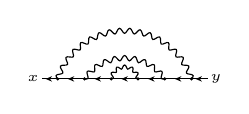
\begin{tikzpicture}[x=0.340cm, y=0.340cm, line width=0.420pt, baseline={([yshift=-0.6ex]0,0)}]
  \draw (-1.500,0.000) -- (-2.500,0.000);
  \fill (-2.119,0.000) -- (-1.881,-0.102) -- (-1.958,0.000) -- (-1.881,0.102) -- cycle;
  \draw (2.500,0.000) -- (1.500,0.000);
  \fill (1.881,0.000) -- (2.119,-0.102) -- (2.042,0.000) -- (2.119,0.102) -- cycle;
  \draw (-0.500,0.000) -- (-1.500,0.000);
  \fill (-1.119,0.000) -- (-0.881,-0.102) -- (-0.958,0.000) -- (-0.881,0.102) -- cycle;
  \draw (1.500,0.000) -- (0.500,0.000);
  \fill (0.881,0.000) -- (1.119,-0.102) -- (1.042,0.000) -- (1.119,0.102) -- cycle;
  \draw (0.500,0.000) -- (-0.500,0.000);
  \fill (-0.119,0.000) -- (0.119,-0.102) -- (0.042,0.000) -- (0.119,0.102) -- cycle;
  \draw plot[smooth, tension=0.7] coordinates {(0.500,0.000) (0.447,0.025) (0.421,0.050) (0.433,0.083) (0.468,0.130) (0.500,0.181) (0.501,0.224) (0.464,0.246) (0.404,0.247) (0.345,0.241) (0.311,0.249) (0.303,0.284) (0.311,0.342) (0.312,0.403) (0.291,0.440) (0.248,0.440) (0.196,0.410) (0.148,0.376) (0.114,0.365) (0.090,0.392) (0.067,0.446) (0.037,0.498) (0.000,0.520) (-0.037,0.498) (-0.067,0.446) (-0.090,0.392) (-0.114,0.365) (-0.148,0.376) (-0.196,0.410) (-0.248,0.440) (-0.291,0.440) (-0.312,0.403) (-0.311,0.342) (-0.303,0.284) (-0.311,0.249) (-0.345,0.241) (-0.404,0.247) (-0.464,0.246) (-0.501,0.224) (-0.500,0.181) (-0.468,0.130) (-0.433,0.083) (-0.421,0.050) (-0.447,0.025) (-0.500,0.000)};
  \draw plot[smooth, tension=0.7] coordinates {(-2.500,0.000) (-2.550,0.068) (-2.560,0.123) (-2.516,0.158) (-2.434,0.176) (-2.352,0.192) (-2.308,0.221) (-2.314,0.275) (-2.356,0.347) (-2.396,0.421) (-2.398,0.477) (-2.349,0.505) (-2.265,0.512) (-2.182,0.516) (-2.134,0.539) (-2.133,0.592) (-2.164,0.670) (-2.193,0.749) (-2.187,0.805) (-2.135,0.826) (-2.051,0.820) (-1.968,0.812) (-1.917,0.828) (-1.908,0.881) (-1.928,0.962) (-1.945,1.044) (-1.931,1.099) (-1.877,1.112) (-1.795,1.095) (-1.714,1.075) (-1.661,1.084) (-1.645,1.135) (-1.652,1.218) (-1.658,1.302) (-1.637,1.354) (-1.581,1.359) (-1.502,1.330) (-1.425,1.299) (-1.371,1.300) (-1.348,1.349) (-1.344,1.432) (-1.337,1.516) (-1.309,1.564) (-1.253,1.562) (-1.179,1.522) (-1.107,1.480) (-1.053,1.473) (-1.023,1.518) (-1.008,1.600) (-0.989,1.682) (-0.954,1.726) (-0.899,1.715) (-0.832,1.665) (-0.766,1.614) (-0.714,1.600) (-0.678,1.640) (-0.651,1.718) (-0.621,1.797) (-0.580,1.835) (-0.527,1.817) (-0.468,1.758) (-0.410,1.698) (-0.361,1.676) (-0.320,1.711) (-0.281,1.785) (-0.241,1.858) (-0.195,1.891) (-0.145,1.865) (-0.094,1.798) (-0.046,1.730) (0.000,1.702) (0.046,1.730) (0.094,1.798) (0.145,1.865) (0.195,1.891) (0.241,1.858) (0.281,1.785) (0.320,1.711) (0.361,1.676) (0.410,1.698) (0.468,1.758) (0.527,1.817) (0.580,1.835) (0.621,1.797) (0.651,1.718) (0.678,1.640) (0.714,1.600) (0.766,1.614) (0.832,1.665) (0.899,1.715) (0.954,1.726) (0.989,1.682) (1.008,1.600) (1.023,1.518) (1.053,1.473) (1.107,1.480) (1.179,1.522) (1.253,1.562) (1.309,1.564) (1.337,1.516) (1.344,1.432) (1.348,1.349) (1.371,1.300) (1.425,1.299) (1.502,1.330) (1.581,1.359) (1.637,1.354) (1.658,1.302) (1.652,1.218) (1.645,1.135) (1.661,1.084) (1.714,1.075) (1.795,1.095) (1.877,1.112) (1.931,1.099) (1.945,1.044) (1.928,0.962) (1.908,0.881) (1.917,0.828) (1.968,0.812) (2.051,0.820) (2.135,0.826) (2.187,0.805) (2.193,0.749) (2.164,0.670) (2.133,0.592) (2.134,0.539) (2.182,0.516) (2.265,0.512) (2.349,0.505) (2.398,0.477) (2.396,0.421) (2.356,0.347) (2.314,0.275) (2.308,0.221) (2.352,0.192) (2.434,0.176) (2.516,0.158) (2.560,0.123) (2.550,0.068) (2.500,0.000)};
  \draw plot[smooth, tension=0.7] coordinates {(1.500,0.000) (1.418,-0.003) (1.369,0.015) (1.364,0.067) (1.386,0.146) (1.406,0.226) (1.394,0.281) (1.340,0.295) (1.259,0.279) (1.179,0.260) (1.127,0.268) (1.111,0.318) (1.118,0.399) (1.121,0.482) (1.098,0.533) (1.042,0.537) (0.966,0.505) (0.892,0.470) (0.840,0.467) (0.814,0.513) (0.804,0.594) (0.791,0.676) (0.758,0.721) (0.702,0.713) (0.634,0.667) (0.569,0.618) (0.518,0.605) (0.484,0.644) (0.458,0.722) (0.428,0.799) (0.387,0.837) (0.334,0.818) (0.276,0.759) (0.222,0.698) (0.175,0.675) (0.133,0.707) (0.092,0.778) (0.048,0.847) (0.000,0.876) (-0.048,0.847) (-0.092,0.778) (-0.133,0.707) (-0.175,0.675) (-0.222,0.698) (-0.276,0.759) (-0.334,0.818) (-0.387,0.837) (-0.428,0.799) (-0.458,0.722) (-0.484,0.644) (-0.518,0.605) (-0.569,0.618) (-0.634,0.667) (-0.702,0.713) (-0.758,0.721) (-0.791,0.676) (-0.804,0.594) (-0.814,0.513) (-0.840,0.467) (-0.892,0.470) (-0.966,0.505) (-1.042,0.537) (-1.098,0.533) (-1.121,0.482) (-1.118,0.399) (-1.111,0.318) (-1.127,0.268) (-1.179,0.260) (-1.259,0.279) (-1.340,0.295) (-1.394,0.281) (-1.406,0.226) (-1.386,0.146) (-1.364,0.067) (-1.369,0.015) (-1.418,-0.003) (-1.500,0.000)};
  \draw (-2.500,0.000) -- (-3.100,0.000);
  \fill (-2.949,0.000) -- (-2.711,-0.102) -- (-2.788,0.000) -- (-2.711,0.102) -- cycle;
  \draw (2.500,0.000) -- (3.100,0.000);
  \fill (2.651,0.000) -- (2.889,-0.102) -- (2.812,0.000) -- (2.889,0.102) -- cycle;
  \fill (-2.500,0.000) circle (0.064);
  \fill (2.500,0.000) circle (0.064);
  \fill (1.500,0.000) circle (0.064);
  \fill (-1.500,0.000) circle (0.064);
  \fill (0.500,0.000) circle (0.064);
  \fill (-0.500,0.000) circle (0.064);
  \node[font=\tiny, inner sep=0pt, anchor=0] at (-3.190,0.000) {$x$};
  \node[font=\tiny, inner sep=0pt, anchor=180] at (3.190,0.000) {$y$};
\end{tikzpicture}}
\diagramgap
\mbox{$\displaystyle -\,$\,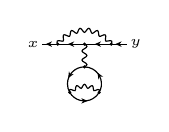
\begin{tikzpicture}[x=0.340cm, y=0.340cm, line width=0.420pt, baseline={([yshift=-0.6ex]0,0)}]
  \draw (0.000,0.000) -- (-1.000,0.000);
  \fill (-0.619,0.000) -- (-0.381,-0.102) -- (-0.458,0.000) -- (-0.381,0.102) -- cycle;
  \draw (1.000,0.000) -- (0.000,0.000);
  \fill (0.381,0.000) -- (0.619,-0.102) -- (0.542,0.000) -- (0.619,0.102) -- cycle;
  \draw (0.550,-1.803) arc[start angle=330.000, end angle=450.000, radius=0.635];
  \fill (0.490,-1.064) -- (0.521,-1.322) -- (0.571,-1.204) -- (0.698,-1.220) -- cycle;
  \draw (0.000,-0.850) arc[start angle=90.000, end angle=210.000, radius=0.635];
  \fill (-0.610,-1.271) -- (-0.402,-1.115) -- (-0.529,-1.131) -- (-0.579,-1.013) -- cycle;
  \draw (-0.550,-1.803) arc[start angle=210.000, end angle=330.000, radius=0.635];
  \fill (0.119,-2.120) -- (-0.119,-2.018) -- (-0.042,-2.120) -- (-0.119,-2.222) -- cycle;
  \draw plot[smooth, tension=0.7] coordinates {(-0.550,-1.803) (-0.560,-1.742) (-0.547,-1.702) (-0.505,-1.695) (-0.447,-1.714) (-0.391,-1.737) (-0.354,-1.738) (-0.337,-1.704) (-0.330,-1.645) (-0.318,-1.585) (-0.292,-1.552) (-0.250,-1.559) (-0.202,-1.597) (-0.158,-1.638) (-0.123,-1.652) (-0.095,-1.627) (-0.068,-1.573) (-0.036,-1.521) (0.000,-1.499) (0.036,-1.521) (0.068,-1.573) (0.095,-1.627) (0.123,-1.652) (0.158,-1.638) (0.202,-1.597) (0.250,-1.559) (0.292,-1.552) (0.318,-1.585) (0.330,-1.645) (0.337,-1.704) (0.354,-1.738) (0.391,-1.737) (0.447,-1.714) (0.505,-1.695) (0.547,-1.702) (0.560,-1.742) (0.550,-1.803)};
  \draw plot[smooth, tension=0.7] coordinates {(-1.000,0.000) (-1.023,0.066) (-1.017,0.113) (-0.972,0.130) (-0.902,0.122) (-0.834,0.110) (-0.792,0.119) (-0.781,0.162) (-0.790,0.230) (-0.796,0.300) (-0.777,0.344) (-0.730,0.349) (-0.665,0.323) (-0.602,0.295) (-0.558,0.293) (-0.537,0.331) (-0.529,0.400) (-0.516,0.469) (-0.488,0.507) (-0.441,0.499) (-0.384,0.458) (-0.330,0.415) (-0.288,0.402) (-0.258,0.434) (-0.233,0.498) (-0.204,0.561) (-0.166,0.591) (-0.122,0.572) (-0.078,0.518) (-0.037,0.462) (0.000,0.439) (0.037,0.462) (0.078,0.518) (0.122,0.572) (0.166,0.591) (0.204,0.561) (0.233,0.498) (0.258,0.434) (0.288,0.402) (0.330,0.415) (0.384,0.458) (0.441,0.499) (0.488,0.507) (0.516,0.469) (0.529,0.400) (0.537,0.331) (0.558,0.293) (0.602,0.295) (0.665,0.323) (0.730,0.349) (0.777,0.344) (0.796,0.300) (0.790,0.230) (0.781,0.162) (0.792,0.119) (0.834,0.110) (0.902,0.122) (0.972,0.130) (1.017,0.113) (1.023,0.066) (1.000,0.000)};
  \draw plot[smooth, tension=0.7] coordinates {(0.000,0.000) (0.065,-0.043) (0.092,-0.085) (0.065,-0.128) (0.000,-0.170) (-0.065,-0.213) (-0.092,-0.255) (-0.065,-0.298) (0.000,-0.340) (0.065,-0.383) (0.092,-0.425) (0.065,-0.468) (0.000,-0.510) (-0.065,-0.553) (-0.092,-0.595) (-0.065,-0.638) (0.000,-0.680) (0.065,-0.723) (0.092,-0.765) (0.065,-0.808) (0.000,-0.850)};
  \draw (-1.000,0.000) -- (-1.600,0.000);
  \fill (-1.449,0.000) -- (-1.211,-0.102) -- (-1.288,0.000) -- (-1.211,0.102) -- cycle;
  \draw (1.000,0.000) -- (1.600,0.000);
  \fill (1.151,0.000) -- (1.389,-0.102) -- (1.312,0.000) -- (1.389,0.102) -- cycle;
  \fill (-1.000,0.000) circle (0.064);
  \fill (1.000,0.000) circle (0.064);
  \fill (0.000,0.000) circle (0.064);
  \fill (0.000,-0.850) circle (0.064);
  \fill (-0.550,-1.803) circle (0.064);
  \fill (0.550,-1.803) circle (0.064);
  \node[font=\tiny, inner sep=0pt, anchor=0] at (-1.690,0.000) {$x$};
  \node[font=\tiny, inner sep=0pt, anchor=180] at (1.690,0.000) {$y$};
\end{tikzpicture}}
\diagramgap
\mbox{$\displaystyle -\,$\,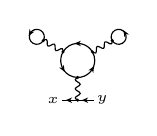
\begin{tikzpicture}[x=0.340cm, y=0.340cm, line width=0.420pt, baseline={([yshift=-0.6ex]0,0)}]
  \draw (-0.550,1.803) arc[start angle=150.000, end angle=270.000, radius=0.635];
  \fill (-0.490,1.064) -- (-0.521,1.322) -- (-0.571,1.204) -- (-0.698,1.220) -- cycle;
  \draw (0.000,0.850) arc[start angle=270.000, end angle=390.000, radius=0.635];
  \fill (0.610,1.271) -- (0.402,1.115) -- (0.529,1.131) -- (0.579,1.013) -- cycle;
  \draw (0.550,1.803) arc[start angle=30.000, end angle=150.000, radius=0.635];
  \fill (-0.119,2.120) -- (0.119,2.018) -- (0.042,2.120) -- (0.119,2.222) -- cycle;
  \draw plot[smooth, tension=0.7] coordinates {(0.000,0.000) (-0.065,0.043) (-0.092,0.085) (-0.065,0.128) (0.000,0.170) (0.065,0.213) (0.092,0.255) (0.065,0.298) (0.000,0.340) (-0.065,0.383) (-0.092,0.425) (-0.065,0.468) (0.000,0.510) (0.065,0.553) (0.092,0.595) (0.065,0.638) (0.000,0.680) (-0.065,0.723) (-0.092,0.765) (-0.065,0.808) (0.000,0.850)};
  \draw plot[smooth, tension=0.7] coordinates {(1.286,2.228) (1.282,2.150) (1.258,2.106) (1.208,2.108) (1.139,2.143) (1.070,2.178) (1.019,2.180) (0.996,2.135) (0.992,2.058) (0.987,1.980) (0.964,1.936) (0.914,1.938) (0.844,1.973) (0.775,2.008) (0.725,2.010) (0.702,1.965) (0.697,1.888) (0.693,1.810) (0.670,1.766) (0.619,1.768) (0.550,1.803)};
  \draw plot[smooth, tension=0.7] coordinates {(-1.286,2.228) (-1.217,2.263) (-1.167,2.265) (-1.143,2.220) (-1.139,2.143) (-1.135,2.065) (-1.111,2.021) (-1.061,2.023) (-0.992,2.058) (-0.922,2.093) (-0.872,2.095) (-0.849,2.050) (-0.844,1.973) (-0.840,1.895) (-0.817,1.851) (-0.766,1.853) (-0.697,1.888) (-0.628,1.923) (-0.578,1.925) (-0.554,1.880) (-0.550,1.803)};
  \draw (1.286,2.228) arc[start angle=210.000, end angle=570.000, radius=0.280];
  \fill (1.711,2.611) -- (1.742,2.353) -- (1.792,2.471) -- (1.919,2.455) -- cycle;
  \draw (-1.286,2.228) arc[start angle=330.000, end angle=690.000, radius=0.280];
  \fill (-1.831,2.404) -- (-1.623,2.560) -- (-1.750,2.544) -- (-1.800,2.662) -- cycle;
  \draw (0.000,0.000) -- (-0.600,0.000);
  \fill (-0.449,0.000) -- (-0.211,-0.102) -- (-0.288,0.000) -- (-0.211,0.102) -- cycle;
  \draw (0.000,0.000) -- (0.600,0.000);
  \fill (0.151,0.000) -- (0.389,-0.102) -- (0.312,0.000) -- (0.389,0.102) -- cycle;
  \fill (0.000,0.000) circle (0.064);
  \fill (1.286,2.228) circle (0.064);
  \fill (-1.286,2.228) circle (0.064);
  \fill (0.000,0.850) circle (0.064);
  \fill (0.550,1.803) circle (0.064);
  \fill (-0.550,1.803) circle (0.064);
  \node[font=\tiny, inner sep=0pt, anchor=0] at (-0.690,0.000) {$x$};
  \node[font=\tiny, inner sep=0pt, anchor=180] at (0.690,0.000) {$y$};
\end{tikzpicture}}
\diagramgap
\mbox{$\displaystyle +\,$\,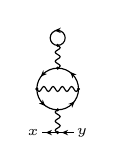
\begin{tikzpicture}[x=0.340cm, y=0.340cm, line width=0.420pt, baseline={([yshift=-0.6ex]0,0)}]
  \draw (-0.778,1.628) arc[start angle=180.000, end angle=270.000, radius=0.778];
  \fill (-0.466,0.993) -- (-0.562,1.234) -- (-0.580,1.107) -- (-0.707,1.090) -- cycle;
  \draw (0.000,0.850) arc[start angle=270.000, end angle=360.000, radius=0.778];
  \fill (0.634,1.162) -- (0.393,1.066) -- (0.520,1.048) -- (0.538,0.921) -- cycle;
  \draw (0.000,2.406) arc[start angle=90.000, end angle=180.000, radius=0.778];
  \fill (-0.634,2.093) -- (-0.393,2.190) -- (-0.520,2.207) -- (-0.538,2.334) -- cycle;
  \draw (0.778,1.628) arc[start angle=0.000, end angle=90.000, radius=0.778];
  \fill (0.466,2.262) -- (0.562,2.021) -- (0.580,2.148) -- (0.707,2.166) -- cycle;
  \draw plot[smooth, tension=0.7] coordinates {(0.000,0.000) (-0.065,0.042) (-0.092,0.085) (-0.065,0.128) (0.000,0.170) (0.065,0.212) (0.092,0.255) (0.065,0.298) (0.000,0.340) (-0.065,0.382) (-0.092,0.425) (-0.065,0.468) (0.000,0.510) (0.065,0.552) (0.092,0.595) (0.065,0.638) (0.000,0.680) (-0.065,0.722) (-0.092,0.765) (-0.065,0.808) (0.000,0.850)};
  \draw plot[smooth, tension=0.7] coordinates {(0.000,3.256) (0.065,3.213) (0.092,3.171) (0.065,3.128) (0.000,3.086) (-0.065,3.043) (-0.092,3.001) (-0.065,2.958) (0.000,2.916) (0.065,2.873) (0.092,2.831) (0.065,2.788) (0.000,2.746) (-0.065,2.703) (-0.092,2.661) (-0.065,2.618) (0.000,2.576) (0.065,2.533) (0.092,2.491) (0.065,2.448) (0.000,2.406)};
  \draw plot[smooth, tension=0.7] coordinates {(0.778,1.628) (0.735,1.562) (0.691,1.534) (0.648,1.562) (0.605,1.628) (0.562,1.694) (0.519,1.721) (0.475,1.694) (0.432,1.628) (0.389,1.562) (0.346,1.534) (0.302,1.562) (0.259,1.628) (0.216,1.694) (0.173,1.721) (0.130,1.694) (0.086,1.628) (0.043,1.562) (0.000,1.534) (-0.043,1.562) (-0.086,1.628) (-0.130,1.694) (-0.173,1.721) (-0.216,1.694) (-0.259,1.628) (-0.302,1.562) (-0.346,1.534) (-0.389,1.562) (-0.432,1.628) (-0.475,1.694) (-0.519,1.721) (-0.562,1.694) (-0.605,1.628) (-0.648,1.562) (-0.691,1.534) (-0.735,1.562) (-0.778,1.628)};
  \draw (0.000,3.256) arc[start angle=270.000, end angle=630.000, radius=0.280];
  \fill (-0.119,3.816) -- (0.119,3.714) -- (0.042,3.816) -- (0.119,3.918) -- cycle;
  \draw (0.000,0.000) -- (-0.600,0.000);
  \fill (-0.449,0.000) -- (-0.211,-0.102) -- (-0.288,0.000) -- (-0.211,0.102) -- cycle;
  \draw (0.000,0.000) -- (0.600,0.000);
  \fill (0.151,0.000) -- (0.389,-0.102) -- (0.312,0.000) -- (0.389,0.102) -- cycle;
  \fill (0.000,0.000) circle (0.064);
  \fill (0.000,3.256) circle (0.064);
  \fill (0.000,0.850) circle (0.064);
  \fill (0.778,1.628) circle (0.064);
  \fill (-0.778,1.628) circle (0.064);
  \fill (0.000,2.406) circle (0.064);
  \node[font=\tiny, inner sep=0pt, anchor=0] at (-0.690,0.000) {$x$};
  \node[font=\tiny, inner sep=0pt, anchor=180] at (0.690,0.000) {$y$};
\end{tikzpicture}}
\diagramgap
\mbox{$\displaystyle -\,$\,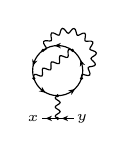
\begin{tikzpicture}[x=0.340cm, y=0.340cm, line width=0.420pt, baseline={([yshift=-0.6ex]0,0)}]
  \draw (-0.890,1.497) arc[start angle=198.000, end angle=270.000, radius=0.936];
  \fill (-0.453,0.959) -- (-0.587,1.181) -- (-0.584,1.053) -- (-0.707,1.016) -- cycle;
  \draw (0.000,0.850) arc[start angle=270.000, end angle=342.000, radius=0.936];
  \fill (0.647,1.099) -- (0.393,1.041) -- (0.516,1.004) -- (0.513,0.876) -- cycle;
  \draw (-0.550,2.543) arc[start angle=126.000, end angle=198.000, radius=0.936];
  \fill (-0.927,1.961) -- (-0.756,2.157) -- (-0.877,2.115) -- (-0.950,2.220) -- cycle;
  \draw (0.890,1.497) arc[start angle=342.000, end angle=414.000, radius=0.936];
  \fill (0.853,2.188) -- (0.830,1.930) -- (0.903,2.035) -- (1.024,1.993) -- cycle;
  \draw (0.550,2.543) arc[start angle=54.000, end angle=126.000, radius=0.936];
  \fill (-0.119,2.721) -- (0.119,2.619) -- (0.042,2.721) -- (0.119,2.823) -- cycle;
  \draw plot[smooth, tension=0.7] coordinates {(0.000,0.000) (-0.065,0.043) (-0.092,0.085) (-0.065,0.128) (0.000,0.170) (0.065,0.213) (0.092,0.255) (0.065,0.298) (0.000,0.340) (-0.065,0.383) (-0.092,0.425) (-0.065,0.468) (0.000,0.510) (0.065,0.553) (0.092,0.595) (0.065,0.638) (0.000,0.680) (-0.065,0.723) (-0.092,0.765) (-0.065,0.808) (0.000,0.850)};
  \draw plot[smooth, tension=0.7] coordinates {(0.890,1.497) (0.890,1.584) (0.909,1.635) (0.963,1.640) (1.048,1.617) (1.136,1.602) (1.195,1.622) (1.206,1.683) (1.177,1.768) (1.143,1.848) (1.139,1.902) (1.187,1.929) (1.273,1.942) (1.360,1.963) (1.407,2.005) (1.392,2.066) (1.332,2.132) (1.268,2.191) (1.243,2.240) (1.276,2.283) (1.350,2.330) (1.421,2.384) (1.446,2.441) (1.409,2.491) (1.327,2.527) (1.244,2.556) (1.202,2.590) (1.215,2.643) (1.264,2.716) (1.307,2.794) (1.308,2.856) (1.253,2.887) (1.164,2.887) (1.076,2.880) (1.024,2.895) (1.015,2.949) (1.030,3.035) (1.038,3.124) (1.014,3.181) (0.952,3.187) (0.869,3.151) (0.792,3.110) (0.738,3.102) (0.708,3.148) (0.688,3.233) (0.660,3.318) (0.614,3.360) (0.555,3.341) (0.494,3.275) (0.440,3.206) (0.394,3.178) (0.348,3.207) (0.295,3.277) (0.235,3.343) (0.176,3.364) (0.130,3.322) (0.100,3.238) (0.079,3.153) (0.048,3.108) (-0.006,3.117) (-0.082,3.159) (-0.164,3.196) (-0.226,3.191) (-0.252,3.134) (-0.245,3.045) (-0.231,2.959) (-0.241,2.905) (-0.294,2.892) (-0.381,2.900) (-0.470,2.901) (-0.525,2.871) (-0.526,2.809) (-0.484,2.730) (-0.436,2.657) (-0.424,2.604) (-0.467,2.570) (-0.550,2.543)};
  \draw plot[smooth, tension=0.7] coordinates {(-0.890,1.497) (-0.894,1.587) (-0.873,1.641) (-0.814,1.645) (-0.730,1.613) (-0.646,1.581) (-0.587,1.585) (-0.566,1.639) (-0.570,1.729) (-0.574,1.819) (-0.553,1.874) (-0.494,1.877) (-0.410,1.845) (-0.326,1.813) (-0.267,1.817) (-0.246,1.871) (-0.250,1.962) (-0.254,2.052) (-0.233,2.106) (-0.174,2.110) (-0.090,2.078) (-0.006,2.046) (0.053,2.049) (0.074,2.104) (0.070,2.194) (0.066,2.284) (0.087,2.339) (0.146,2.342) (0.230,2.310) (0.314,2.278) (0.373,2.282) (0.394,2.336) (0.390,2.426) (0.386,2.517) (0.407,2.571) (0.466,2.575) (0.550,2.543)};
  \draw (0.000,0.000) -- (-0.600,0.000);
  \fill (-0.449,0.000) -- (-0.211,-0.102) -- (-0.288,0.000) -- (-0.211,0.102) -- cycle;
  \draw (0.000,0.000) -- (0.600,0.000);
  \fill (0.151,0.000) -- (0.389,-0.102) -- (0.312,0.000) -- (0.389,0.102) -- cycle;
  \fill (0.000,0.000) circle (0.064);
  \fill (0.000,0.850) circle (0.064);
  \fill (0.890,1.497) circle (0.064);
  \fill (-0.890,1.497) circle (0.064);
  \fill (0.550,2.543) circle (0.064);
  \fill (-0.550,2.543) circle (0.064);
  \node[font=\tiny, inner sep=0pt, anchor=0] at (-0.690,0.000) {$x$};
  \node[font=\tiny, inner sep=0pt, anchor=180] at (0.690,0.000) {$y$};
\end{tikzpicture}}
\diagramgap
\mbox{$\displaystyle +\,$\,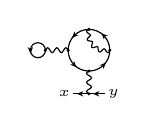
\begin{tikzpicture}[x=0.340cm, y=0.340cm, line width=0.420pt, baseline={([yshift=-0.6ex]0,0)}]
  \draw (-0.778,1.628) arc[start angle=180.000, end angle=270.000, radius=0.778];
  \fill (-0.466,0.993) -- (-0.562,1.234) -- (-0.580,1.107) -- (-0.707,1.090) -- cycle;
  \draw (0.000,0.850) arc[start angle=270.000, end angle=360.000, radius=0.778];
  \fill (0.634,1.162) -- (0.393,1.066) -- (0.520,1.048) -- (0.538,0.921) -- cycle;
  \draw (0.000,2.406) arc[start angle=90.000, end angle=180.000, radius=0.778];
  \fill (-0.634,2.093) -- (-0.393,2.190) -- (-0.520,2.207) -- (-0.538,2.334) -- cycle;
  \draw (0.778,1.628) arc[start angle=0.000, end angle=90.000, radius=0.778];
  \fill (0.466,2.262) -- (0.562,2.021) -- (0.580,2.148) -- (0.707,2.166) -- cycle;
  \draw plot[smooth, tension=0.7] coordinates {(0.778,1.628) (0.753,1.565) (0.717,1.536) (0.674,1.553) (0.631,1.605) (0.595,1.659) (0.563,1.683) (0.528,1.664) (0.484,1.616) (0.434,1.572) (0.388,1.562) (0.357,1.597) (0.343,1.662) (0.335,1.727) (0.318,1.763) (0.278,1.762) (0.217,1.740) (0.152,1.723) (0.106,1.734) (0.095,1.780) (0.112,1.844) (0.134,1.905) (0.135,1.946) (0.099,1.963) (0.034,1.971) (-0.031,1.985) (-0.066,2.016) (-0.056,2.062) (-0.011,2.112) (0.036,2.156) (0.055,2.191) (0.031,2.223) (-0.023,2.259) (-0.075,2.302) (-0.092,2.345) (-0.062,2.381) (0.000,2.406)};
  \draw plot[smooth, tension=0.7] coordinates {(0.000,0.000) (-0.065,0.042) (-0.092,0.085) (-0.065,0.128) (0.000,0.170) (0.065,0.212) (0.092,0.255) (0.065,0.298) (0.000,0.340) (-0.065,0.382) (-0.092,0.425) (-0.065,0.468) (0.000,0.510) (0.065,0.552) (0.092,0.595) (0.065,0.638) (0.000,0.680) (-0.065,0.722) (-0.092,0.765) (-0.065,0.808) (0.000,0.850)};
  \draw plot[smooth, tension=0.7] coordinates {(-1.628,1.628) (-1.585,1.693) (-1.543,1.720) (-1.500,1.693) (-1.458,1.628) (-1.415,1.563) (-1.373,1.536) (-1.330,1.563) (-1.288,1.628) (-1.245,1.693) (-1.203,1.720) (-1.160,1.693) (-1.118,1.628) (-1.075,1.563) (-1.033,1.536) (-0.990,1.563) (-0.948,1.628) (-0.905,1.693) (-0.863,1.720) (-0.820,1.693) (-0.778,1.628)};
  \draw (-1.628,1.628) arc[start angle=0.000, end angle=360.000, radius=0.280];
  \fill (-2.188,1.508) -- (-2.086,1.747) -- (-2.188,1.670) -- (-2.290,1.747) -- cycle;
  \draw (0.000,0.000) -- (-0.600,0.000);
  \fill (-0.449,0.000) -- (-0.211,-0.102) -- (-0.288,0.000) -- (-0.211,0.102) -- cycle;
  \draw (0.000,0.000) -- (0.600,0.000);
  \fill (0.151,0.000) -- (0.389,-0.102) -- (0.312,0.000) -- (0.389,0.102) -- cycle;
  \fill (0.000,0.000) circle (0.064);
  \fill (-1.628,1.628) circle (0.064);
  \fill (0.000,0.850) circle (0.064);
  \fill (0.778,1.628) circle (0.064);
  \fill (-0.778,1.628) circle (0.064);
  \fill (0.000,2.406) circle (0.064);
  \node[font=\tiny, inner sep=0pt, anchor=0] at (-0.690,0.000) {$x$};
  \node[font=\tiny, inner sep=0pt, anchor=180] at (0.690,0.000) {$y$};
\end{tikzpicture}}
\diagramgap
\mbox{$\displaystyle -\,$\,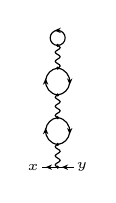
\begin{tikzpicture}[x=0.340cm, y=0.340cm, line width=0.420pt, baseline={([yshift=-0.6ex]0,0)}]
  \draw (0.000,1.850) arc[start angle=83.974, end angle=-83.974, radius=0.503];
  \fill (0.450,1.231) -- (0.552,1.469) -- (0.450,1.392) -- (0.348,1.469) -- cycle;
  \draw (0.000,0.850) arc[start angle=263.974, end angle=96.026, radius=0.503];
  \fill (-0.450,1.469) -- (-0.552,1.231) -- (-0.450,1.308) -- (-0.348,1.231) -- cycle;
  \draw (0.000,2.700) arc[start angle=263.974, end angle=96.026, radius=0.503];
  \fill (-0.450,3.319) -- (-0.552,3.081) -- (-0.450,3.158) -- (-0.348,3.081) -- cycle;
  \draw (0.000,3.700) arc[start angle=83.974, end angle=-83.974, radius=0.503];
  \fill (0.450,3.081) -- (0.552,3.319) -- (0.450,3.242) -- (0.348,3.319) -- cycle;
  \draw plot[smooth, tension=0.7] coordinates {(0.000,0.000) (-0.065,0.042) (-0.092,0.085) (-0.065,0.128) (0.000,0.170) (0.065,0.212) (0.092,0.255) (0.065,0.298) (0.000,0.340) (-0.065,0.382) (-0.092,0.425) (-0.065,0.468) (0.000,0.510) (0.065,0.552) (0.092,0.595) (0.065,0.638) (0.000,0.680) (-0.065,0.722) (-0.092,0.765) (-0.065,0.808) (0.000,0.850)};
  \draw plot[smooth, tension=0.7] coordinates {(0.000,4.550) (0.065,4.508) (0.092,4.465) (0.065,4.422) (0.000,4.380) (-0.065,4.338) (-0.092,4.295) (-0.065,4.252) (0.000,4.210) (0.065,4.168) (0.092,4.125) (0.065,4.082) (0.000,4.040) (-0.065,3.998) (-0.092,3.955) (-0.065,3.912) (0.000,3.870) (0.065,3.828) (0.092,3.785) (0.065,3.742) (0.000,3.700)};
  \draw plot[smooth, tension=0.7] coordinates {(0.000,1.850) (-0.065,1.892) (-0.092,1.935) (-0.065,1.978) (0.000,2.020) (0.065,2.062) (0.092,2.105) (0.065,2.148) (0.000,2.190) (-0.065,2.232) (-0.092,2.275) (-0.065,2.318) (0.000,2.360) (0.065,2.403) (0.092,2.445) (0.065,2.488) (0.000,2.530) (-0.065,2.573) (-0.092,2.615) (-0.065,2.658) (0.000,2.700)};
  \draw (0.000,4.550) arc[start angle=270.000, end angle=630.000, radius=0.280];
  \fill (-0.119,5.110) -- (0.119,5.008) -- (0.042,5.110) -- (0.119,5.212) -- cycle;
  \draw (0.000,0.000) -- (-0.600,0.000);
  \fill (-0.449,0.000) -- (-0.211,-0.102) -- (-0.288,0.000) -- (-0.211,0.102) -- cycle;
  \draw (0.000,0.000) -- (0.600,0.000);
  \fill (0.151,0.000) -- (0.389,-0.102) -- (0.312,0.000) -- (0.389,0.102) -- cycle;
  \fill (0.000,0.000) circle (0.064);
  \fill (0.000,4.550) circle (0.064);
  \fill (0.000,0.850) circle (0.064);
  \fill (0.000,1.850) circle (0.064);
  \fill (0.000,3.700) circle (0.064);
  \fill (0.000,2.700) circle (0.064);
  \node[font=\tiny, inner sep=0pt, anchor=0] at (-0.690,0.000) {$x$};
  \node[font=\tiny, inner sep=0pt, anchor=180] at (0.690,0.000) {$y$};
\end{tikzpicture}}
\diagramgap
\mbox{$\displaystyle -\,$\,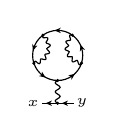
\begin{tikzpicture}[x=0.340cm, y=0.340cm, line width=0.420pt, baseline={([yshift=-0.6ex]0,0)}]
  \draw (-0.890,1.497) arc[start angle=198.000, end angle=270.000, radius=0.936];
  \fill (-0.453,0.959) -- (-0.587,1.181) -- (-0.584,1.053) -- (-0.707,1.016) -- cycle;
  \draw (0.000,0.850) arc[start angle=270.000, end angle=342.000, radius=0.936];
  \fill (0.647,1.099) -- (0.393,1.041) -- (0.516,1.004) -- (0.513,0.876) -- cycle;
  \draw (-0.550,2.543) arc[start angle=126.000, end angle=198.000, radius=0.936];
  \fill (-0.927,1.961) -- (-0.756,2.157) -- (-0.877,2.115) -- (-0.950,2.220) -- cycle;
  \draw plot[smooth, tension=0.7] coordinates {(-0.890,1.497) (-0.864,1.546) (-0.838,1.570) (-0.806,1.557) (-0.764,1.519) (-0.718,1.484) (-0.678,1.479) (-0.654,1.511) (-0.646,1.568) (-0.643,1.624) (-0.630,1.656) (-0.595,1.658) (-0.541,1.641) (-0.485,1.629) (-0.446,1.640) (-0.438,1.680) (-0.454,1.735) (-0.475,1.787) (-0.477,1.822) (-0.446,1.838) (-0.390,1.845) (-0.334,1.858) (-0.304,1.884) (-0.312,1.923) (-0.350,1.967) (-0.391,2.005) (-0.407,2.037) (-0.385,2.064) (-0.338,2.094) (-0.292,2.129) (-0.276,2.166) (-0.300,2.198) (-0.353,2.221) (-0.406,2.239) (-0.433,2.261) (-0.425,2.295) (-0.395,2.342) (-0.368,2.393) (-0.368,2.433) (-0.404,2.451) (-0.461,2.451) (-0.517,2.445) (-0.551,2.453) (-0.558,2.487) (-0.550,2.543)};
  \draw (0.890,1.497) arc[start angle=342.000, end angle=414.000, radius=0.936];
  \fill (0.853,2.188) -- (0.830,1.930) -- (0.903,2.035) -- (1.024,1.993) -- cycle;
  \draw plot[smooth, tension=0.7] coordinates {(0.890,1.497) (0.852,1.453) (0.815,1.439) (0.784,1.465) (0.764,1.519) (0.749,1.573) (0.729,1.602) (0.695,1.596) (0.646,1.568) (0.594,1.544) (0.554,1.547) (0.537,1.584) (0.541,1.641) (0.550,1.697) (0.544,1.731) (0.510,1.740) (0.454,1.735) (0.397,1.735) (0.362,1.755) (0.362,1.795) (0.390,1.845) (0.421,1.892) (0.430,1.925) (0.403,1.948) (0.350,1.967) (0.298,1.991) (0.274,2.023) (0.291,2.060) (0.338,2.094) (0.386,2.123) (0.408,2.150) (0.393,2.181) (0.353,2.221) (0.316,2.265) (0.308,2.304) (0.338,2.330) (0.395,2.342) (0.451,2.348) (0.482,2.363) (0.481,2.398) (0.461,2.451) (0.446,2.506) (0.455,2.545) (0.494,2.556) (0.550,2.543)};
  \draw (0.550,2.543) arc[start angle=54.000, end angle=126.000, radius=0.936];
  \fill (-0.119,2.721) -- (0.119,2.619) -- (0.042,2.721) -- (0.119,2.823) -- cycle;
  \draw plot[smooth, tension=0.7] coordinates {(0.000,0.000) (-0.065,0.043) (-0.092,0.085) (-0.065,0.128) (0.000,0.170) (0.065,0.213) (0.092,0.255) (0.065,0.298) (0.000,0.340) (-0.065,0.383) (-0.092,0.425) (-0.065,0.468) (0.000,0.510) (0.065,0.553) (0.092,0.595) (0.065,0.638) (0.000,0.680) (-0.065,0.723) (-0.092,0.765) (-0.065,0.808) (0.000,0.850)};
  \draw (0.000,0.000) -- (-0.600,0.000);
  \fill (-0.449,0.000) -- (-0.211,-0.102) -- (-0.288,0.000) -- (-0.211,0.102) -- cycle;
  \draw (0.000,0.000) -- (0.600,0.000);
  \fill (0.151,0.000) -- (0.389,-0.102) -- (0.312,0.000) -- (0.389,0.102) -- cycle;
  \fill (0.000,0.000) circle (0.064);
  \fill (0.000,0.850) circle (0.064);
  \fill (0.890,1.497) circle (0.064);
  \fill (-0.890,1.497) circle (0.064);
  \fill (0.550,2.543) circle (0.064);
  \fill (-0.550,2.543) circle (0.064);
  \node[font=\tiny, inner sep=0pt, anchor=0] at (-0.690,0.000) {$x$};
  \node[font=\tiny, inner sep=0pt, anchor=180] at (0.690,0.000) {$y$};
\end{tikzpicture}}
\diagramgap
\mbox{$\displaystyle +\,$\,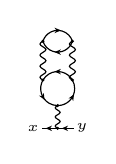
\begin{tikzpicture}[x=0.340cm, y=0.340cm, line width=0.420pt, baseline={([yshift=-0.6ex]0,0)}]
  \draw (-0.550,1.803) arc[start angle=150.000, end angle=270.000, radius=0.635];
  \fill (-0.490,1.064) -- (-0.521,1.322) -- (-0.571,1.204) -- (-0.698,1.220) -- cycle;
  \draw (0.000,0.850) arc[start angle=270.000, end angle=390.000, radius=0.635];
  \fill (0.610,1.271) -- (0.402,1.115) -- (0.529,1.131) -- (0.579,1.013) -- cycle;
  \draw (0.550,1.803) arc[start angle=30.000, end angle=150.000, radius=0.635];
  \fill (-0.119,2.120) -- (0.119,2.018) -- (0.042,2.120) -- (0.119,2.222) -- cycle;
  \draw (-0.550,3.253) arc[start angle=162.811, end angle=17.189, radius=0.576];
  \fill (0.119,3.658) -- (-0.119,3.760) -- (-0.042,3.658) -- (-0.119,3.556) -- cycle;
  \draw (0.550,3.253) arc[start angle=342.811, end angle=197.189, radius=0.576];
  \fill (-0.119,2.847) -- (0.119,2.745) -- (0.042,2.847) -- (0.119,2.949) -- cycle;
  \draw plot[smooth, tension=0.7] coordinates {(0.000,0.000) (-0.065,0.043) (-0.092,0.085) (-0.065,0.128) (0.000,0.170) (0.065,0.213) (0.092,0.255) (0.065,0.298) (0.000,0.340) (-0.065,0.383) (-0.092,0.425) (-0.065,0.468) (0.000,0.510) (0.065,0.553) (0.092,0.595) (0.065,0.638) (0.000,0.680) (-0.065,0.723) (-0.092,0.765) (-0.065,0.808) (0.000,0.850)};
  \draw plot[smooth, tension=0.7] coordinates {(0.550,1.803) (0.471,1.854) (0.438,1.906) (0.471,1.958) (0.550,2.010) (0.629,2.062) (0.662,2.113) (0.629,2.165) (0.550,2.217) (0.471,2.269) (0.438,2.320) (0.471,2.372) (0.550,2.424) (0.629,2.476) (0.662,2.528) (0.629,2.579) (0.550,2.631) (0.471,2.683) (0.438,2.735) (0.471,2.787) (0.550,2.838) (0.629,2.890) (0.662,2.942) (0.629,2.994) (0.550,3.045) (0.471,3.097) (0.438,3.149) (0.471,3.201) (0.550,3.253)};
  \draw plot[smooth, tension=0.7] coordinates {(-0.550,1.803) (-0.629,1.854) (-0.662,1.906) (-0.629,1.958) (-0.550,2.010) (-0.471,2.062) (-0.438,2.113) (-0.471,2.165) (-0.550,2.217) (-0.629,2.269) (-0.662,2.320) (-0.629,2.372) (-0.550,2.424) (-0.471,2.476) (-0.438,2.528) (-0.471,2.579) (-0.550,2.631) (-0.629,2.683) (-0.662,2.735) (-0.629,2.787) (-0.550,2.838) (-0.471,2.890) (-0.438,2.942) (-0.471,2.994) (-0.550,3.045) (-0.629,3.097) (-0.662,3.149) (-0.629,3.201) (-0.550,3.253)};
  \draw (0.000,0.000) -- (-0.600,0.000);
  \fill (-0.449,0.000) -- (-0.211,-0.102) -- (-0.288,0.000) -- (-0.211,0.102) -- cycle;
  \draw (0.000,0.000) -- (0.600,0.000);
  \fill (0.151,0.000) -- (0.389,-0.102) -- (0.312,0.000) -- (0.389,0.102) -- cycle;
  \fill (0.000,0.000) circle (0.064);
  \fill (0.000,0.850) circle (0.064);
  \fill (0.550,1.803) circle (0.064);
  \fill (-0.550,1.803) circle (0.064);
  \fill (0.550,3.253) circle (0.064);
  \fill (-0.550,3.253) circle (0.064);
  \node[font=\tiny, inner sep=0pt, anchor=0] at (-0.690,0.000) {$x$};
  \node[font=\tiny, inner sep=0pt, anchor=180] at (0.690,0.000) {$y$};
\end{tikzpicture}}
\diagramgap
\mbox{$\displaystyle +\,$\,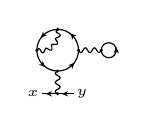
\begin{tikzpicture}[x=0.340cm, y=0.340cm, line width=0.420pt, baseline={([yshift=-0.6ex]0,0)}]
  \draw (-0.778,1.628) arc[start angle=180.000, end angle=270.000, radius=0.778];
  \fill (-0.466,0.993) -- (-0.562,1.234) -- (-0.580,1.107) -- (-0.707,1.090) -- cycle;
  \draw (0.000,0.850) arc[start angle=270.000, end angle=360.000, radius=0.778];
  \fill (0.634,1.162) -- (0.393,1.066) -- (0.520,1.048) -- (0.538,0.921) -- cycle;
  \draw (0.000,2.406) arc[start angle=90.000, end angle=180.000, radius=0.778];
  \fill (-0.634,2.093) -- (-0.393,2.190) -- (-0.520,2.207) -- (-0.538,2.334) -- cycle;
  \draw plot[smooth, tension=0.7] coordinates {(-0.778,1.628) (-0.730,1.672) (-0.693,1.688) (-0.663,1.662) (-0.631,1.605) (-0.593,1.550) (-0.551,1.529) (-0.513,1.556) (-0.484,1.616) (-0.461,1.678) (-0.436,1.709) (-0.397,1.698) (-0.343,1.662) (-0.284,1.631) (-0.237,1.631) (-0.215,1.673) (-0.217,1.740) (-0.224,1.804) (-0.216,1.844) (-0.176,1.852) (-0.112,1.844) (-0.045,1.843) (-0.004,1.865) (-0.003,1.912) (-0.034,1.971) (-0.071,2.025) (-0.081,2.064) (-0.050,2.089) (0.011,2.112) (0.072,2.141) (0.099,2.179) (0.078,2.221) (0.023,2.259) (-0.034,2.291) (-0.060,2.321) (-0.044,2.358) (0.000,2.406)};
  \draw (0.778,1.628) arc[start angle=0.000, end angle=90.000, radius=0.778];
  \fill (0.466,2.262) -- (0.562,2.021) -- (0.580,2.148) -- (0.707,2.166) -- cycle;
  \draw plot[smooth, tension=0.7] coordinates {(0.000,0.000) (-0.065,0.042) (-0.092,0.085) (-0.065,0.128) (0.000,0.170) (0.065,0.212) (0.092,0.255) (0.065,0.298) (0.000,0.340) (-0.065,0.382) (-0.092,0.425) (-0.065,0.468) (0.000,0.510) (0.065,0.552) (0.092,0.595) (0.065,0.638) (0.000,0.680) (-0.065,0.722) (-0.092,0.765) (-0.065,0.808) (0.000,0.850)};
  \draw plot[smooth, tension=0.7] coordinates {(1.628,1.628) (1.585,1.563) (1.543,1.536) (1.500,1.563) (1.458,1.628) (1.415,1.693) (1.373,1.720) (1.330,1.693) (1.288,1.628) (1.245,1.563) (1.203,1.536) (1.160,1.563) (1.118,1.628) (1.075,1.693) (1.033,1.720) (0.990,1.693) (0.948,1.628) (0.905,1.563) (0.863,1.536) (0.820,1.563) (0.778,1.628)};
  \draw (1.628,1.628) arc[start angle=180.000, end angle=540.000, radius=0.280];
  \fill (2.188,1.747) -- (2.086,1.508) -- (2.188,1.586) -- (2.290,1.508) -- cycle;
  \draw (0.000,0.000) -- (-0.600,0.000);
  \fill (-0.449,0.000) -- (-0.211,-0.102) -- (-0.288,0.000) -- (-0.211,0.102) -- cycle;
  \draw (0.000,0.000) -- (0.600,0.000);
  \fill (0.151,0.000) -- (0.389,-0.102) -- (0.312,0.000) -- (0.389,0.102) -- cycle;
  \fill (0.000,0.000) circle (0.064);
  \fill (1.628,1.628) circle (0.064);
  \fill (0.000,0.850) circle (0.064);
  \fill (0.778,1.628) circle (0.064);
  \fill (-0.778,1.628) circle (0.064);
  \fill (0.000,2.406) circle (0.064);
  \node[font=\tiny, inner sep=0pt, anchor=0] at (-0.690,0.000) {$x$};
  \node[font=\tiny, inner sep=0pt, anchor=180] at (0.690,0.000) {$y$};
\end{tikzpicture}}
\diagramgap
\mbox{$\displaystyle -\,$\,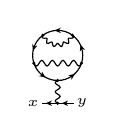
\begin{tikzpicture}[x=0.340cm, y=0.340cm, line width=0.420pt, baseline={([yshift=-0.6ex]0,0)}]
  \draw (-0.890,1.497) arc[start angle=198.000, end angle=270.000, radius=0.936];
  \fill (-0.453,0.959) -- (-0.587,1.181) -- (-0.584,1.053) -- (-0.707,1.016) -- cycle;
  \draw (0.000,0.850) arc[start angle=270.000, end angle=342.000, radius=0.936];
  \fill (0.647,1.099) -- (0.393,1.041) -- (0.516,1.004) -- (0.513,0.876) -- cycle;
  \draw (-0.550,2.543) arc[start angle=126.000, end angle=198.000, radius=0.936];
  \fill (-0.927,1.961) -- (-0.756,2.157) -- (-0.877,2.115) -- (-0.950,2.220) -- cycle;
  \draw (0.890,1.497) arc[start angle=342.000, end angle=414.000, radius=0.936];
  \fill (0.853,2.188) -- (0.830,1.930) -- (0.903,2.035) -- (1.024,1.993) -- cycle;
  \draw (0.550,2.543) arc[start angle=54.000, end angle=126.000, radius=0.936];
  \fill (-0.119,2.721) -- (0.119,2.619) -- (0.042,2.721) -- (0.119,2.823) -- cycle;
  \draw plot[smooth, tension=0.7] coordinates {(0.550,2.543) (0.580,2.493) (0.582,2.453) (0.547,2.433) (0.490,2.430) (0.434,2.433) (0.400,2.422) (0.395,2.388) (0.407,2.333) (0.413,2.276) (0.398,2.238) (0.358,2.234) (0.305,2.256) (0.255,2.282) (0.220,2.286) (0.201,2.257) (0.189,2.202) (0.171,2.148) (0.141,2.120) (0.103,2.133) (0.064,2.175) (0.029,2.219) (0.000,2.238) (-0.029,2.219) (-0.064,2.175) (-0.103,2.133) (-0.141,2.120) (-0.171,2.148) (-0.189,2.202) (-0.201,2.257) (-0.220,2.286) (-0.255,2.282) (-0.305,2.256) (-0.358,2.234) (-0.398,2.238) (-0.413,2.276) (-0.407,2.333) (-0.395,2.388) (-0.400,2.422) (-0.434,2.433) (-0.490,2.430) (-0.547,2.433) (-0.582,2.453) (-0.580,2.493) (-0.550,2.543)};
  \draw plot[smooth, tension=0.7] coordinates {(0.000,0.000) (-0.065,0.043) (-0.092,0.085) (-0.065,0.128) (0.000,0.170) (0.065,0.213) (0.092,0.255) (0.065,0.298) (0.000,0.340) (-0.065,0.383) (-0.092,0.425) (-0.065,0.468) (0.000,0.510) (0.065,0.553) (0.092,0.595) (0.065,0.638) (0.000,0.680) (-0.065,0.723) (-0.092,0.765) (-0.065,0.808) (0.000,0.850)};
  \draw plot[smooth, tension=0.7] coordinates {(0.890,1.497) (0.840,1.421) (0.791,1.390) (0.742,1.421) (0.692,1.497) (0.643,1.572) (0.593,1.603) (0.544,1.572) (0.494,1.497) (0.445,1.421) (0.396,1.390) (0.346,1.421) (0.297,1.497) (0.247,1.572) (0.198,1.603) (0.148,1.572) (0.099,1.497) (0.049,1.421) (0.000,1.390) (-0.049,1.421) (-0.099,1.497) (-0.148,1.572) (-0.198,1.603) (-0.247,1.572) (-0.297,1.497) (-0.346,1.421) (-0.396,1.390) (-0.445,1.421) (-0.494,1.497) (-0.544,1.572) (-0.593,1.603) (-0.643,1.572) (-0.692,1.497) (-0.742,1.421) (-0.791,1.390) (-0.840,1.421) (-0.890,1.497)};
  \draw (0.000,0.000) -- (-0.600,0.000);
  \fill (-0.449,0.000) -- (-0.211,-0.102) -- (-0.288,0.000) -- (-0.211,0.102) -- cycle;
  \draw (0.000,0.000) -- (0.600,0.000);
  \fill (0.151,0.000) -- (0.389,-0.102) -- (0.312,0.000) -- (0.389,0.102) -- cycle;
  \fill (0.000,0.000) circle (0.064);
  \fill (0.000,0.850) circle (0.064);
  \fill (0.890,1.497) circle (0.064);
  \fill (-0.890,1.497) circle (0.064);
  \fill (0.550,2.543) circle (0.064);
  \fill (-0.550,2.543) circle (0.064);
  \node[font=\tiny, inner sep=0pt, anchor=0] at (-0.690,0.000) {$x$};
  \node[font=\tiny, inner sep=0pt, anchor=180] at (0.690,0.000) {$y$};
\end{tikzpicture}}
\diagramgap
\mbox{$\displaystyle +\,$\,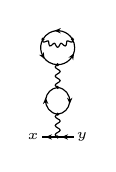
\begin{tikzpicture}[x=0.340cm, y=0.340cm, line width=0.420pt, baseline={([yshift=-0.6ex]0,0)}]
  \draw (0.000,1.850) arc[start angle=83.974, end angle=-83.974, radius=0.503];
  \fill (0.450,1.231) -- (0.552,1.469) -- (0.450,1.392) -- (0.348,1.469) -- cycle;
  \draw (0.000,0.850) arc[start angle=263.974, end angle=96.026, radius=0.503];
  \fill (-0.450,1.469) -- (-0.552,1.231) -- (-0.450,1.308) -- (-0.348,1.231) -- cycle;
  \draw (-0.550,3.653) arc[start angle=150.000, end angle=270.000, radius=0.635];
  \fill (-0.490,2.914) -- (-0.521,3.172) -- (-0.571,3.054) -- (-0.698,3.070) -- cycle;
  \draw (0.000,2.700) arc[start angle=270.000, end angle=390.000, radius=0.635];
  \fill (0.610,3.121) -- (0.402,2.965) -- (0.529,2.981) -- (0.579,2.863) -- cycle;
  \draw (0.550,3.653) arc[start angle=30.000, end angle=150.000, radius=0.635];
  \fill (-0.119,3.970) -- (0.119,3.868) -- (0.042,3.970) -- (0.119,4.072) -- cycle;
  \draw plot[smooth, tension=0.7] coordinates {(0.550,3.653) (0.560,3.592) (0.547,3.552) (0.505,3.545) (0.447,3.564) (0.391,3.587) (0.354,3.588) (0.337,3.554) (0.330,3.495) (0.318,3.435) (0.292,3.402) (0.250,3.409) (0.202,3.447) (0.158,3.488) (0.123,3.502) (0.095,3.477) (0.068,3.423) (0.036,3.371) (0.000,3.349) (-0.036,3.371) (-0.068,3.423) (-0.095,3.477) (-0.123,3.502) (-0.158,3.488) (-0.202,3.447) (-0.250,3.409) (-0.292,3.402) (-0.318,3.435) (-0.330,3.495) (-0.337,3.554) (-0.354,3.588) (-0.391,3.587) (-0.447,3.564) (-0.505,3.545) (-0.547,3.552) (-0.560,3.592) (-0.550,3.653)};
  \draw plot[smooth, tension=0.7] coordinates {(0.000,0.000) (-0.065,0.042) (-0.092,0.085) (-0.065,0.128) (0.000,0.170) (0.065,0.212) (0.092,0.255) (0.065,0.298) (0.000,0.340) (-0.065,0.382) (-0.092,0.425) (-0.065,0.468) (0.000,0.510) (0.065,0.552) (0.092,0.595) (0.065,0.638) (0.000,0.680) (-0.065,0.722) (-0.092,0.765) (-0.065,0.808) (0.000,0.850)};
  \draw plot[smooth, tension=0.7] coordinates {(0.000,1.850) (-0.065,1.892) (-0.092,1.935) (-0.065,1.978) (0.000,2.020) (0.065,2.062) (0.092,2.105) (0.065,2.148) (0.000,2.190) (-0.065,2.232) (-0.092,2.275) (-0.065,2.318) (0.000,2.360) (0.065,2.403) (0.092,2.445) (0.065,2.488) (0.000,2.530) (-0.065,2.573) (-0.092,2.615) (-0.065,2.658) (0.000,2.700)};
  \draw (0.000,0.000) -- (-0.600,0.000);
  \fill (-0.449,0.000) -- (-0.211,-0.102) -- (-0.288,0.000) -- (-0.211,0.102) -- cycle;
  \draw (0.000,0.000) -- (0.600,0.000);
  \fill (0.151,0.000) -- (0.389,-0.102) -- (0.312,0.000) -- (0.389,0.102) -- cycle;
  \fill (0.000,0.000) circle (0.064);
  \fill (0.000,0.850) circle (0.064);
  \fill (0.000,1.850) circle (0.064);
  \fill (0.000,2.700) circle (0.064);
  \fill (0.550,3.653) circle (0.064);
  \fill (-0.550,3.653) circle (0.064);
  \node[font=\tiny, inner sep=0pt, anchor=0] at (-0.690,0.000) {$x$};
  \node[font=\tiny, inner sep=0pt, anchor=180] at (0.690,0.000) {$y$};
\end{tikzpicture}}
